\documentclass{article}

\usepackage{iclr2026_conference}
\usepackage{makecell}
\bibliographystyle{unsrtnat}
\newtheorem{definition}{Definition}
\newtheorem{proposition}{Proposition}
\newtheorem{repeatedproposition}{Proposition}
\newenvironment{restatedproposition}[1]{%
\renewcommand{\therepeatedproposition}{\ref{#1}}%
\begin{repeatedproposition}}{\end{repeatedproposition}}
\newtheorem{property}{Property}
\newtheorem{example}{Example}
\usepackage{amsmath}
\usepackage{algorithm}
\newcommand{\isometrypursuit}{{\sc IsometryPursuit}}
\newcommand{\brute}{{\sc BruteSearch}}
\newcommand{\greedy}{{\sc GreedySearch}}
\newcommand{\backwardgreedy}{{\sc BackwardGreedySearch}}
\newcommand{\forwardbackward}{{\sc SwapSearch}}
\newcommand{\tsip}{{\sc TwoStageIsometryPursuit}}
\usepackage[font=small]{caption}
\captionsetup[algorithm]{labelformat=empty}
% \usepackage{algpseudocode}
\usepackage{algorithmic}
\usepackage{subcaption}
\usepackage{graphicx}
\usepackage[utf8]{inputenc} % allow utf-8 input
\usepackage[T1]{fontenc}    % use 8-bit T1 fonts
\usepackage{hyperref}       % hyperlinks
\usepackage{url}            % simple URL typesetting
\usepackage{booktabs}       % professional-quality tables
\usepackage{amsfonts}       % blackboard math symbols
\usepackage{nicefrac}       % compact symbols for 1/2, etc.
\usepackage{microtype}      % microtypography
\usepackage{xcolor}         % colors
\usepackage{tikz-cd}
\newenvironment{proof}{\paragraph{Proof:}}{\hfill$\square$}

\usepackage{afterpage}

\newcommand{\M}{\mathcal{M}}
\newcommand{\N}{\mathcal{N}}


\title{Isometry Pursuit: Convex Recovery of Orthonormal Column Submatrices}

%\author{%
%  Samson Koelle \\
%  Amazon  \\
%  koelle@amazon.com
%  \And
%  Marina Meila \\
%  Department of Statistics\\
%  University of Washington \\
%  mmp@uw.edu 
%}

\begin{document}

\maketitle 

\begin{abstract}
Isometry pursuit is a convex algorithm for identifying orthonormal column-submatrices of wide matrices.
It consists of a vector normalization followed by multitask basis pursuit.
Our theoretical results include characterization of the attractive geometric properties of the basis pursuit loss and a proof that any orthonormal column-submatrix is contained among the multitask basis-pursuit minimizers.
Our empirical results show that or problems involving coordinate selection and diversification, it offers a synergistic alternative to greedy and brute force search.
\end{abstract}

\footnotetext[1]{Work conducted outside of Amazon.}

\section{Introduction}
\label{sec:introduction}

Many real-world problems may be abstracted as selecting a subset of the columns of a matrix representing stochastic observations or analytically exact data.
This paper focuses on a simple such problem.
Given a rank $D$ matrix $ X \in \mathbb R^{D \times P}$ with $P > D$, select a square submatrix $ X_{. S}$ where subset $ S \subset [P]$ satisfies $| S| = D$ that is as isometric as possible.



This problem arises in feature learning because while the coordinate functions of a given feature space may have no intrinsic meaning, it is often possible to generate a dictionary of interpretable features for consideration as potential parametrizing coordinates.
When this is the case, selection of candidate interpretable features as coordinates can take the above form.
Isometric embeddings - data mappings that compress high-dimensional distributions into low dimensions while preserving distances and angles on the data surface - have differentials that are isometric matrices.
Thus, selecting isometric embeddings from without dictionaries of putative coordinates can be cast as a linear isometric submatrix coordinate selection problem.
Identification of such coordinates generally aids mechanistic understanding, generative control, and statistical efficiency.

This paper takes an optimization perspective on the problem of selecting isometric submatrices.
The background develops the the problem from the perspective of non-linear embeddings.
However, the focus switches to a purely linear algebraic perspective in the remainder of the paper.

The main contribution of this paper is to show that an adapted version of the multitask basis pursuit feature learning algorithm in \citet{Koelle2024-no} is a convex alternative isometry selection algorithm.
This enables identification of low-dimensional coordinates within a Jacobian that preserve the original geometry of the data manifold under mapping given by the flow lines 
This algorithm - \isometrypursuit~ - is multitask basis pursuit applied to an appropriately normalized $ X$ selects orthonormal submatrices.
Given vectors in $\mathbb R^D$, the normalization log-symmetrizes length and favors those closer to unit length, while basis pursuit favors those which are orthogonal.
Our theoretical results formalize this intuition, and show the usefulness of \isometrypursuit~ as a trimming procedure prior to brute force search for diversification and interpretable coordinate selection.
It is an alternative to greedy coordinate selection approaches such as those in \citet{5895106, NEURIPS2019_6a10bbd4, Kohli2021-lr, Jones2007-uc}.

\begin{figure}[t]
\centering
\subcaptionbox{Raw data\label{fig:data}}[0.18\textwidth]
{\includegraphics[width=\linewidth]{/Users/samsonkoelle/isometry-pursuit/figures/data.png}}\hfill
\subcaptionbox{Isometric subset\label{fig:selection}}[0.18\textwidth]
{\includegraphics[width=\linewidth]{/Users/samsonkoelle/isometry-pursuit/figures/selection.png}}\hfill
\subcaptionbox{Normalization\label{fig:normalization}}[0.18\textwidth]
{\includegraphics[width=\linewidth]{/Users/samsonkoelle/isometry-pursuit/figures/normalization.png}}\hfill
\subcaptionbox{Candidate losses for $D=1$\label{fig:loss_1d_all}}[0.42\textwidth]
{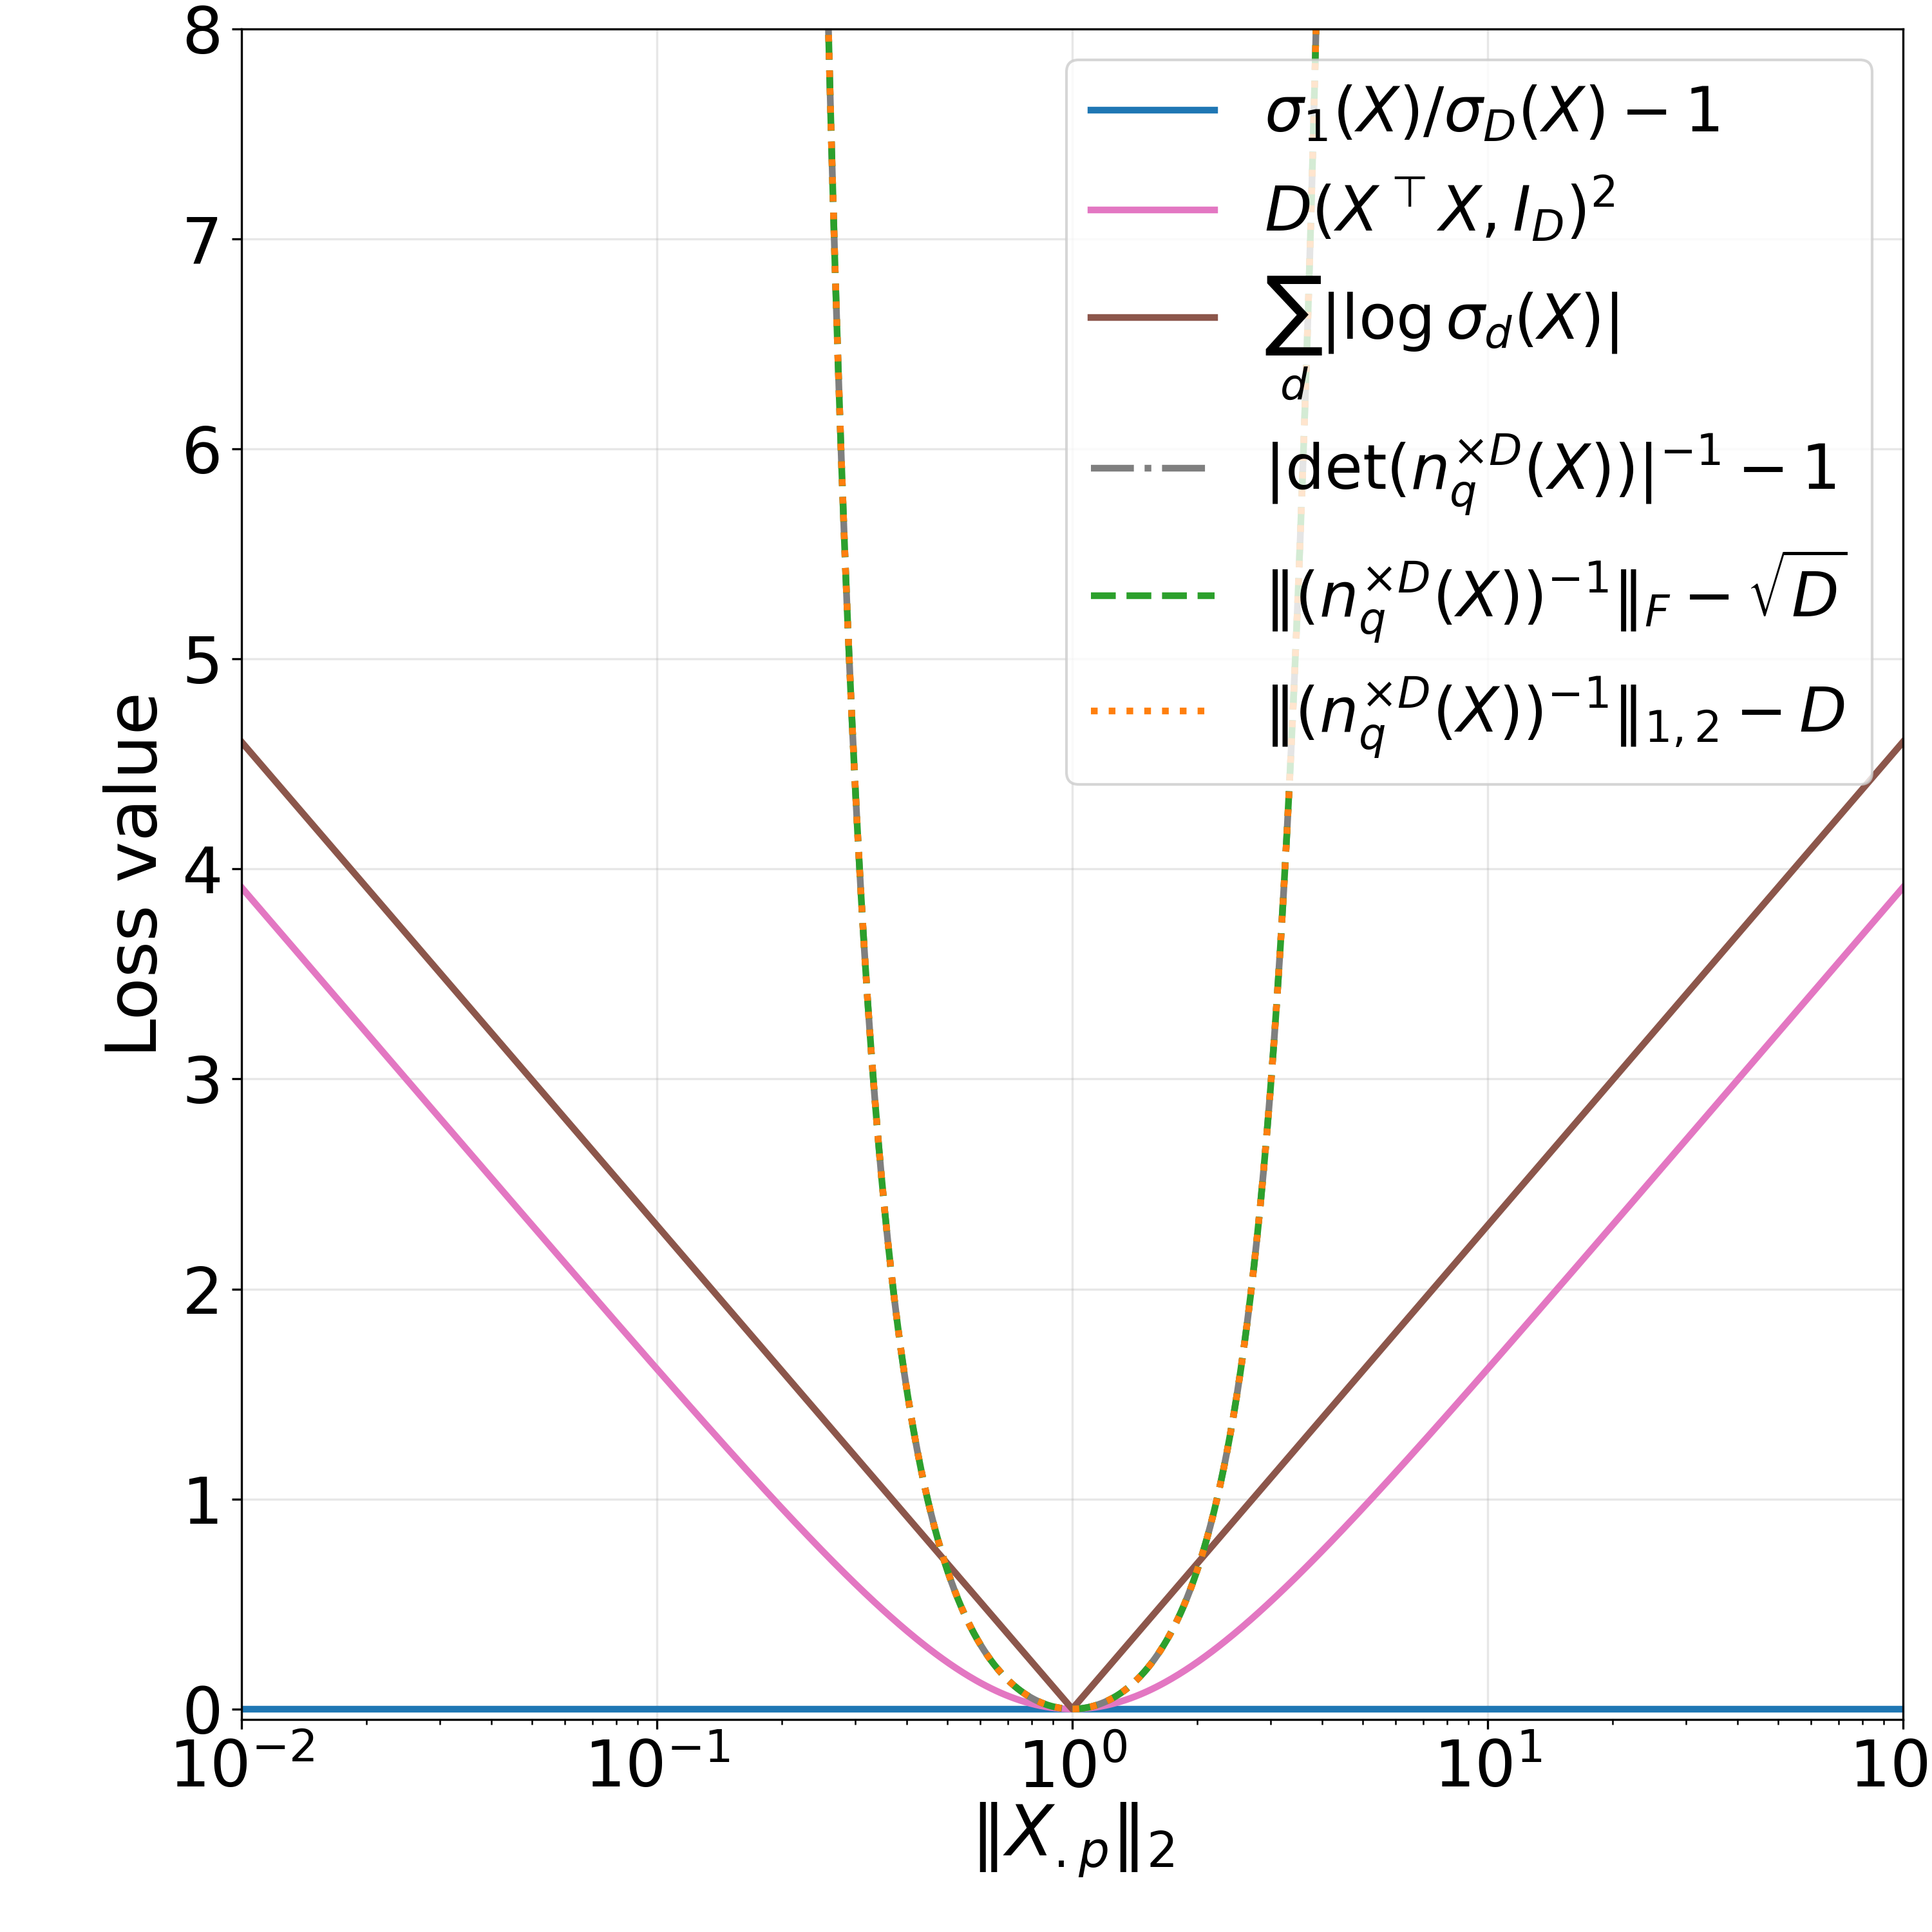
\includegraphics[width=\linewidth]{../figures/loss_1d_all.png}}
\caption{The isometric-submatrix selection problem and candidate losses.
\ref{fig:data} Raw data $X$.
\ref{fig:selection} An isometric subset.
\ref{fig:normalization} Symmetric normalization makes vectors nearest unit
length the longest.
\ref{fig:loss_1d_all} One-dimensional candidate losses for $X=[[r]]$; the red
vertical dashed line marks $r=1$.
\label{fig:losses}
}
\end{figure}
 %\footnotetext[2]{Code is available at \url{https://anonymous.4open.science/r/isometry-pursuit-8FC4/README.md}.}

\section{Background}

Our goal is, given a matrix $ X \in \mathbb R^{D \times P}$, to select a subset $ S \subset [P]$ with $| S| = D$ such that $X_{.  S}$ is as orthonormal as possible in a computationally efficient way.
Figure \ref{fig:data} and \ref{fig:selection} provide a visual depiction of this problem when $D=2$ and $P=30$.
We motivate this problem from the perspective of non-linear embeddings.

\subsection{Isometry}

Isometries are a classical object in numerical linear algebra and geometry.
They preserve distances and angles, and such can be used faithfully for subsequent human or algorithmic analysis.
This motivates embedding algorithms such as Local Tangent Space Alignment \citep{ZhangZ:04}, Multidimensional Scaling \citep{ChenBuja:localMDS09}, and Isomap \citep{tenenbaum2000ggf}.

\begin{definition}
\label{def:isometry}
A matrix $X \in \mathbb R^{D \times D}$ is an \textbf{isometry} or, equivalently, \textbf{unitary} if
$X X^T = I_D$.

\end{definition}

\begin{proposition}
\label{prop:orthonormal_spectrum}
The singular values $\sigma_1(X) \dots \sigma_D(X)$ are equal to $1$ if and only if $X$ is an isometry.
\end{proposition}
\begin{proposition}
\label{prop:orthonormal_basis}
If $P = D$, the component vectors $X_{.1} \dots X_{.D} \in \mathbb R^D$ form an isometry if and only if, for all $d, d' \in [D], \langle X_{.d}, X_{.d'} \rangle = \begin{cases}
1 \; d = d' \\ 
0 \; d \neq d' 
\end{cases}$.
\end{proposition}

\begin{definition}
The \textbf{differential} of a smooth map $\phi:\mathcal M \to \mathcal N$ between $D$ dimensional manifolds $\M \subseteq \mathbb R^B$ and $\N \subseteq \mathbb R^P$ is a map in tangent bases $x_1 \dots x_{D}$ of $T_\xi \M$ and $y_1 \dots y_{D}$ of $T_{\phi(\xi)} \N$ consisting of entries
\begin{align}
\label{eq:diff}
D\phi(\xi)_{ij} = \langle y_i, \frac{\partial \phi}{\partial x_j} \rangle (\xi)
\end{align}
\end{definition}

\begin{definition}
\label{def:isometric_at_a_point}
A map $\phi$ between $D$ dimensional submanifolds is an \textbf{isometry at a point} $\xi \in \mathcal M$ if $D \phi (\xi)$ is an isometry.
\end{definition}

\begin{definition}
\label{def:conformal_at_a_point}
A map $\phi$ between $D$ dimensional submanifolds is \textbf{conformal at a point} $\xi \in \mathcal M$ if there exists a scalar $\lambda(\xi) > 0$ such that
${D \phi (\xi)}^T D \phi (\xi) = \lambda(\xi) I_D$.
\end{definition}

\begin{proposition}
\label{prop:distance_differential_isometry}
Let $\phi:\mathcal M \to \mathcal N$ be a bijection between connected $D$-dimensional Riemannian submanifolds.
\begin{align}
d_\mathcal N(\phi(\xi), \phi(\xi')) = d_\mathcal M(\xi, \xi'),
\end{align}
if and only if $\phi$ is smooth and is an isometry at every point \citep[Problem~6-7]{Lee2018-rm}.
\end{proposition}

\begin{table}[t]
\centering
\tiny
\setlength{\tabcolsep}{2pt}
\begin{tabular}{@{}>{\raggedright\arraybackslash}p{\dimexpr0.17\textwidth-1.5\tabcolsep\relax}>{\centering\arraybackslash}p{\dimexpr0.20\textwidth-1.5\tabcolsep\relax}>{\raggedright\arraybackslash}p{\dimexpr0.46\textwidth-1.5\tabcolsep\relax}>{\centering\arraybackslash}p{\dimexpr0.17\textwidth-1.5\tabcolsep\relax}@{}}
\toprule
\textbf{Reference} & \textbf{Variable} & \textbf{Loss} & \textbf{Algorithm} \\
\midrule
\citet{NEURIPS2019_6a10bbd4} & $S \in \binom{[P]}{M}$ & $\displaystyle
-\frac{1}{N}\sum_{n=1}^N
\log
\frac{
\det\!\left(Df_{.S}(\xi_n)^T Df_{.S}(\xi_n)\right)^{1/2}
}{
\prod_{s \in S} \|Df_{.s}(\xi_n)\|_2
}$
 & \makecell{BRUTE /\\FORWARD GREEDY} \\
\citet{Kohli2021-lr} & $S \in \binom{[P]}{D}$ & $\displaystyle
\frac{\sigma_1(Df_{.S}(\xi))}{\sigma_D(Df_{.S}(\xi))}$ & FORWARD GREEDY \\
\citet{Koelle2024-no} & $\beta \in \mathbb R^{N\times P\times D}$ & $\begin{aligned}
\frac{1}{2}\sum_{n=1}^N
\|I_d- Df (\xi_n) \beta_{n..} \|_F^2 \\ + \lambda \sqrt{ND}\sum_{p=1}^P
\left(\sum_{n=1}^N \sum_{d=1}^D \beta_{npd}^2\right)^{1/2}
\end{aligned}$ & FISTA \\
\bottomrule
\end{tabular}
\caption{Dictionary-based manifold learning losses. We set the eigenfunction
penalty to $0$ for \citet{NEURIPS2019_6a10bbd4} to emphasize the geometric
condition. Chen--Meil\u{a} normalize the rows of the selected tangent-basis
matrix in our transposed convention; the resulting criterion favors functional
independence rather than orthogonality of the selected gradients.
Chen--Meil\u{a} use brute search at fixed cardinality and also
give a brute-$D$ initialization followed by forward-greedy additions.
\citet{Kohli2021-lr} use forward-greedy selection; their loss is shown in
its infinitesimal form from Proposition~\ref{prop:distortion_is_condition_number}.
The neighborhood distortion and proof are given in
Section~\ref{proof:distortion_is_condition_number}.}
\label{tab:losses}
\end{table}

\subsection{Coordinate selection}

More recently, methods for selecting $D$ coordinates from a dictionary $f_{1:P}$ of candidate features have emerged \citep{Kohli2021-lr, Koelle2022-ju, Koelle2024-}.
Loss functions for isometry vary along many axes.
For example, functions may be measured at a single point \citep{Kohli2021-lr} or over an entire dataset \citep{Koelle2022-ju, Koelle2024-no, NEURIPS2019_6a10bbd4}.
The loss function may make use of either linearized or non-linearized objectives.
Objectives can be computed analytically or from numerical methods.
Isometry may be relaxed as optimization target to the weaker notion of conformalness or embedding.

The dictionary-based coordinate search problem best subset selection problem is
\begin{align}
\label{prog:function_best_subset_selection}
\arg \min_{ S \in \binom{[P]}{D}} \ell ( f_{. S})
\end{align}
where $\ell$ is some loss function that measures isometricness of a selected functional subset $f_{. S}$.
Often, this problem is linearized via defining a loss at a point $\xi$ as 
\begin{align}
\label{prog:linearized_best_subset_selection}
\ell  = \ell'(D f_{. S}(\xi))
\end{align}
where $\ell'$ is now a loss function that measures the orthonormalness of the matrix $D f_{. S}(\xi)$.
Non-linear objectives are often gradient estimators of linearized objectives, and so the distinction is smaller than it may appear.
\begin{proposition}
\label{prop:distortion_is_condition_number}
If $f_{.S}$ is continuously differentiable near $\xi$ and $Df_{.S}(\xi)$ is
invertible, then, with $\operatorname{Distortion}$ defined in
Section~\ref{proof:distortion_is_condition_number} and $B_{\mathcal M}(\xi,\varepsilon)$ denoting
the geodesic ball of radius $\varepsilon$ centered at $\xi$,
\begin{align}
\lim_{\varepsilon\to 0}
\operatorname{Distortion}\!\left(f_{.S},B_{\mathcal M}(\xi,\varepsilon)\right)
=\frac{\sigma_1\!\left(Df_{.S}(\xi)\right)}
       {\sigma_D\!\left(Df_{.S}(\xi)\right)},
\end{align}
the condition number of $Df_{.S}(\xi)$ \citep{GolubWilkinson-condition,Boyd2004-ql}.
\end{proposition}
\begin{proposition}
This is minimized by conformal maps.
\end{proposition}
Furthermore, linearization can have computational advantages.
For example, \citet{Koelle2024-no} computes $Df_{.S}(\xi)$ via automatic differentiation.

\subsection{Isometry losses}

So far in this section, we have established the notion and desireableness of isometric embedding, and reviewed algorithms used for selecting column-submatrices that for conditions weaker than isometry.
We now turn our review to the linear algebra literature.

\begin{table}[t]
\centering
\scriptsize
\setlength{\tabcolsep}{2pt}
\begin{tabular}{@{}>{\raggedright\arraybackslash}p{0.20\textwidth}>{\raggedright\arraybackslash}p{0.31\textwidth}*{4}{>{\centering\arraybackslash}p{0.105\textwidth}}@{}}
\toprule
\textbf{Loss function} & \textbf{Definition} & \makecell{\textbf{Property}\\\textbf{\ref{property:rotation_invariance}}\\Rotation} & \makecell{\textbf{Property}\\\textbf{\ref{property:unique_isometry_minimum}}\\Isometry\\minimum} & \makecell{\textbf{Property}\\\textbf{\ref{property:log_symmetry}}\\Column\\symmetry} & \makecell{\textbf{Property}\\\textbf{\ref{property:pathwise}}\\Column\\mono.} \\
\midrule
\makecell[l]{Distortion\\\citep{Kohli2021-lr}} & $\sigma_1(X) / \sigma_D(X) - 1$ & Yes & No & No & No \\
Spectral divergence & $\sum_{d=1}^D g(\sigma_d(X))$ & Yes & Yes & No & No \\
Normalized determinant volume & $\left|\det\left(n_q^{\times D}(X)\right)\right|^{-1}-1$ & Yes & Yes & Yes & Yes \\
Frob. pseudoinverse & $\|(n_q^{\times D}(X))^{-1}\|_F-\sqrt{D}$ & Yes & Yes & Yes & Yes \\
\isometrypursuit & $\|(n_q^{\times D}(X))^{-1}\|_{1,2}-D$ & Yes & Yes & Yes & Yes \\
\bottomrule
\end{tabular}
\caption{Matrix losses on square, full-rank matrices $X\in\mathbb R^{D\times D}$,
$D\geq2$, using the normalization profile $q$ in \eqref{eq:normalization}.
The last four columns correspond to Properties~\ref{property:rotation_invariance}--\ref{property:pathwise}.
For the spectral divergence, $g$ is continuously differentiable,
$g(1)=0$, $g(t)=g(t^{-1})$, and $g'(t)>0$ for $t>1$.
Its failures of column symmetry and monotonicity are shown in
Section~\ref{proof:inverse_symmetry_impossibility}.
Property~\ref{property:unique_isometry_minimum} means that the minimizers are
exactly the isometries, not that a single matrix minimizes the loss.}
\label{tab:loss_functions}
\end{table}

\begin{property}[Rotation invariance]
\label{property:rotation_invariance}
A matrix loss $\ell$ is rotation invariant if, for every orthonormal $U \in \mathbb R^{D \times D}$,
\begin{align}
\ell(UX) = \ell(X).
\end{align}
\end{property}

\begin{property}[Unique isometry minimum]
\label{property:unique_isometry_minimum}
A matrix loss $\ell$ is uniquely minimized by isometries if
\begin{align}
\arg \min_X \ell(X) = \{X : XX^T = I_D\}.
\end{align}
\end{property}

\begin{definition}{\citet{Sra2011-sdivergence}}
The \textbf{S-divergence} $D(P,P')$ on positive definite matrices $P,P'$ is given by 
\begin{align}
D(P,P') = (\log \det (\frac{P + P'}{2}) - \frac{1}{2}\log \det(PP'))^{\frac{1}{2}}.
\end{align}
\end{definition}
\begin{proposition}
\label{prop:sdiv_singular_values}
If $X^T X$ is positive definite, then
\begin{align}
D(X^T X,I_D)^2
&= \sum_{d=1}^D \log \frac{\sigma_d(X) + \sigma_d(X)^{-1}}{2}.
\end{align}
\end{proposition}
\begin{proposition}
\label{prop:sdiv_minimized_by_isometries}
If $X^T X$ is positive definite, then $D(X^T X,I_D)^2$ is uniquely minimized by isometric matrices.
\end{proposition}
See \citep{Cichocki2014-logdet} for a more extensive discussion of other matrix divergences.
% Alpha, beta, and gamma divergences are investigated in more detail in
% https://chatgpt.com/share/6af66679-66e8-83e8-a7cc-3c64ee5ad07e
% We omit that discussion here for brevity.
In Section \ref{sec:method}, we will examine matrix loss functions capable of selecting isometric submatrices based on their singular values from a generic perspective.
%TODO: explain how works for PSD not just PD.

\subsection{Sparse convex coordinate selection}
\label{sec:sparse_convex_coordinate_selection}

Equipped with a function $\ell$ that is minimized by an isometry, objective functions like \ref{prog:function_best_subset_selection} may be optimized in a variety of ways.
Brute force algorithms consider all possible solutions are guaranteed to find the global minimum, but have the often prohibitive time complexity $O(C_\ell P^D)$ where $C_\ell$ is the cost of evaluating $\ell$.
In contrast, greedy algorithms consist of iteratively adding one element at a time to $ S$.
This algorithms have time complexity $O(C_\ell PD)$ and so are computationally more efficient than brute force algorithms, but can get stuck in local minima.
Formal definitions are given in Section \ref{sec:algorithms}.

Sometimes, it is possible to introduce an objective which convexifies problems of the above form \citep{Liberti2004-iu, Abdi2013-th, Zhou2021-zz}.
\begin{align}
\arg \min_{\beta \in \mathbb R^P : y  = X\beta} \rho(\beta) 
\end{align}
for an overcomplete regression problem $y = X \beta$ is a classic example \citep{Chen2001-hh}.
Overcomplete regression problems are distinguished by the fact that $P > D$ and so the solution $\beta$ is not unique.
When $\rho(\beta) = \|\beta\|_0$, this non-convex problem searches directly for a sparsest representing subset.
However, when $\rho(\beta) =\|\beta\|_1$, the problem is a convex relaxation and may be solved efficiently e.g. via interior-point methods.
Because the $\ell_1$ objective is scale-sensitive, this relaxation is geometrically meaningful for coordinate selection only after normalizing the columns of $X$ so that sparsity is not confounded with column length.
See \citet{JMLR:v23:21-0420} for a recent discussion.

\section{Method}
\label{sec:method}

The contributions of this paper is that we introduce an $\ell$ uniquely minimized by isometries that is convex in its parameters, induces sparsity, and is more appropriate than S-divergence when an isometric submatrix is not present in that it always favors vectors of unit length.
We call this $\ell$ multitask basis pursuit rather than group basis pursuite \citep{Koelle2022-ju,Szeghy2022-ri} since grouping is dependent only on the structure of matrix-valued response variable $I_D$.
We show that this approach, used to select independent dictionary elements in \citet{Koelle2022-ju, Koelle2024-no}, is in fact capable of usefully solving the more specific problem of selecting pointwise isometries from a dictionary.
We justify this approach in two ways.
First, we should that this loss and its {\it method of frames} analog have intuitively preferable geometric properties to S-divergence and other singular-value based losses.
Second, we exhibit the usefulness of this basis pursuit approach for convexifying the coordinate selection problem.

\subsection{The problem with singular values}
\label{sec:singular_value_problem}

$D(X^TX, I_D)$ is not the only function of $X$ minimized uniquely by orthonormal matrices and invariant under rotation.
Consider functions of the form
\begin{align}
\label{eq:gt_loss}
\ell(X) = \sum_{d = 1}^D g(\sigma_d(X)),
\end{align}
where $g:\mathbb R^+\to\mathbb R^+$ is a scalar penalty.
Any $g$ uniquely minimized at $1$ provides a suitable penalty on the singular values.
The following properties are also desirable.
\begin{property}[Monotonicity away from one]
\label{property:scalar_monotonicity}
A scalar penalty $g$ is monotone away from one if
\[
g'(t)
\begin{cases}
<0 \; : \; 0 < t < 1 \\
=0 \; : \; t = 1 \\
>0 \; : \; t > 1.
\end{cases}
\]
\end{property}

\begin{property}[Log symmetry]
\label{property:log_symmetry}
A scalar penalty $g$ is log-symmetric if
$g(t)=g(t^{-1})$ for every $t>0$.
\end{property}

\begin{property}[Column-rescaling monotonicity]
\label{property:pathwise}
A matrix loss $\ell$ is column-rescaling monotone if, for every
column $x_{.d}$,
\[
\frac{\partial\ell}{\partial\|x_{.d}\|_2}
\begin{cases}
<0 \; : \; \|x_{.d}\|_2 < 1 \\
=0 \; : \; \|x_{.d}\|_2 = 1 \\
>0 \; : \; \|x_{.d}\|_2 > 1.
\end{cases}
\]
\end{property}

Unfortunately, we show the following proposition.
\begin{proposition}
\label{prop:log_svd_bad}
There does not exist a $g$ such that $\ell = \sum_{d=1}^D g( \sigma_d(X))$ such that $\ell$ satisfies Property \ref{property:pathwise} and Property \ref{property:log_symmetry}.
\end{proposition}
A suitable matrix for which no $g$ can be chosen such that a log det divergence satisfies Properties \ref{property:pathwise} and \ref{property:log_symmetry} is shown in Section \ref{sec:nearly_colinear_singular_values}.
Figure \ref{fig:loss_1d_all} gives graphs of candidate losses when $D=1$.
A view of the loss landscape for this matrix is shown in Figure \ref{fig:loss_3d_equicorr_landscapes}.
The level sets of the log det losses are not tangent to length at $r = 1$.
This means that given an angle loss can actually be decreased by shrinking a vector away from length $1$.
This is an intuitively bad property for a loss that is supposed to prefer orthonormal matrices.

\subsection{Normalization}
\label{sec:normalization}

Although starting from singular values is bad in the sense of Proposition \ref{prop:log_svd_bad}, other losses do satisfy this property.
These losses arise from the intuition that we can shrink vectors away from length $1$ according to a symmetric scalar penalty.
Since basis pursuit methods tend to select longer vectors, selection of orthonormal submatrices requires normalization such that both long and short candidate basis vectors are penalized in the subsequent regression.
Then, we can apply some loss function to the rescaled matrix that satisfies Property \ref{property:pathwise}.

The obvious symmetric penalty for deviation from unit length is
$\max(t,t^{-1})$, but it is not differentiable at $t=1$.
We replace the maximum by its smooth LogSumExp relaxation
\citep{Boyd2004-ql}
\begin{align}
a(t)=\log\left(e^t+e^{t^{-1}}\right).
\end{align}
This scalar penalty satisfies Properties \ref{property:scalar_monotonicity} and
\ref{property:log_symmetry}.  Since $a(1)=\log(2e)$, exponentiating its
negative centered value gives the normalization profile
\begin{align}
q(t)
&=\exp\left(a(1)-a(t)\right)
=\frac{2e}{e^t+e^{t^{-1}}}.
\label{eq:normalization}
\end{align}
Thus $q(1)=1$, while $q(t)<1$ for $t\neq1$.

\begin{definition}
We define the \textbf{symmetric normalization}
\begin{align}
n_q: \mathbb R^D \setminus \{0\} &\to \mathbb R^D \\
v &\mapsto \frac{q(\|v\|_2)}{\|v\|_2}v .
\end{align}
\label{def:symmetric_normalization}
\end{definition}

\begin{proposition}
\label{prop:normalization_logsumexp}
The inverse profile $1/q$ is the normalized exponential of the LogSumExp
relaxation of $\max(t,t^{-1})$.
\end{proposition}

This choice of $q$ has some additional useful properties.

\begin{proposition}
For $q$ defined in \eqref{eq:normalization}, $-\log q$ is convex.
\end{proposition}

\begin{proposition}
The function $q$ defined in \eqref{eq:normalization} is smooth on $\mathbb R^+$.
\end{proposition}

\begin{proposition}
For $q$ defined in \eqref{eq:normalization}, $\log q(t)$ decays linearly in $t$ as $t \to \infty$ and in $t^{-1}$ as $t \to 0$.
\end{proposition}

We plot the effect of this normalization on our example data in Figure \ref{fig:normalization}.
% why are these important
% Compared with other functions like $\text{cosh}$

\subsection{Normalized spectral losses}

Many matrix functions applied to suitably normalized matrices are uniquely minimized by orthonormal matrices.
Two examples are the inverse determinant and the Frobenius norm of the inverse.
Let $N=n_q^{\times D}(X)$ be square and full rank.
\begin{proposition}[Normalized spectral losses]
\label{prop:normalized_spectral_losses}
Let $h:(0,\infty)\to\mathbb R$ be twice differentiable with
$h'(u)<0$ and $h''(u)>0$ for every $u>0$.  Then
\begin{align}
L_h(X)
=\sum_{d=1}^D h\!\left(\sigma_d(N)^2\right)-D h(1)
\end{align}
satisfies $L_h(X)\geq0$, with equality if and only if $X^\top X=I_D$, and
satisfies Property \ref{property:pathwise}.  In particular, these conclusions
hold for the losses in Propositions
\ref{prop:determinant_singular_values} and
\ref{prop:frobenius_inverse_singular_values}.
\end{proposition}
\begin{proposition}[Inverse determinant]
\label{prop:determinant_singular_values}
The inverse determinant $|\det N|^{-1}$ induces the same ordering as $L_h$ with $h(u)=-\tfrac12\log u$.
\end{proposition}
\begin{proposition}[Inverse Frobenius norm]
\label{prop:frobenius_inverse_singular_values}
The inverse Frobenius norm $\|N^{-1}\|_F$ induces the same ordering as $L_h$ with $h(u)=u^{-1}-1$.
\end{proposition}
Writing $a_d=-\log\sigma_d(N)$, the determinant loss sums $a_d$, while the
centered frame loss sums $e^{2a_d}-1$; the two are proportional near
$a_d=0$, but the frame penalty grows exponentially as a singular direction
collapses.  The frame objective also extends
directly to an overcomplete normalized dictionary: replacing $\|B\|_F$ by
$\|B\|_{1,2}$ under the same constraint $NB=I_D$ yields \isometrypursuit.
%When the columns of $x$ are so normalized, then both the determinant and trace of $X^TX$ are maximized by orthonormal matrices.
%By Proposition \ref{prop:orthonormal_spectrum}, we can see that $\ell$ is uniquely maximized by orthonormal matrices.
%Moreover, $g$ is convex, and $\ell( X^{-1}) = \ell( X)$ when $X$ is invertible.
The stationarity equation in $D=2$ is solved by $g(t)=|\log t|$, whereas the
same $g$ fails in $D=3$, so it would be disingenuous to show the $D=3$
landscape without introducing the $D=3$ example.

\begin{figure}[t]
\centering
\begin{subfigure}[t]{0.49\textwidth}
\centering
\begingroup
\setlength{\tabcolsep}{1pt}
\begin{tabular}{@{}cc@{}}
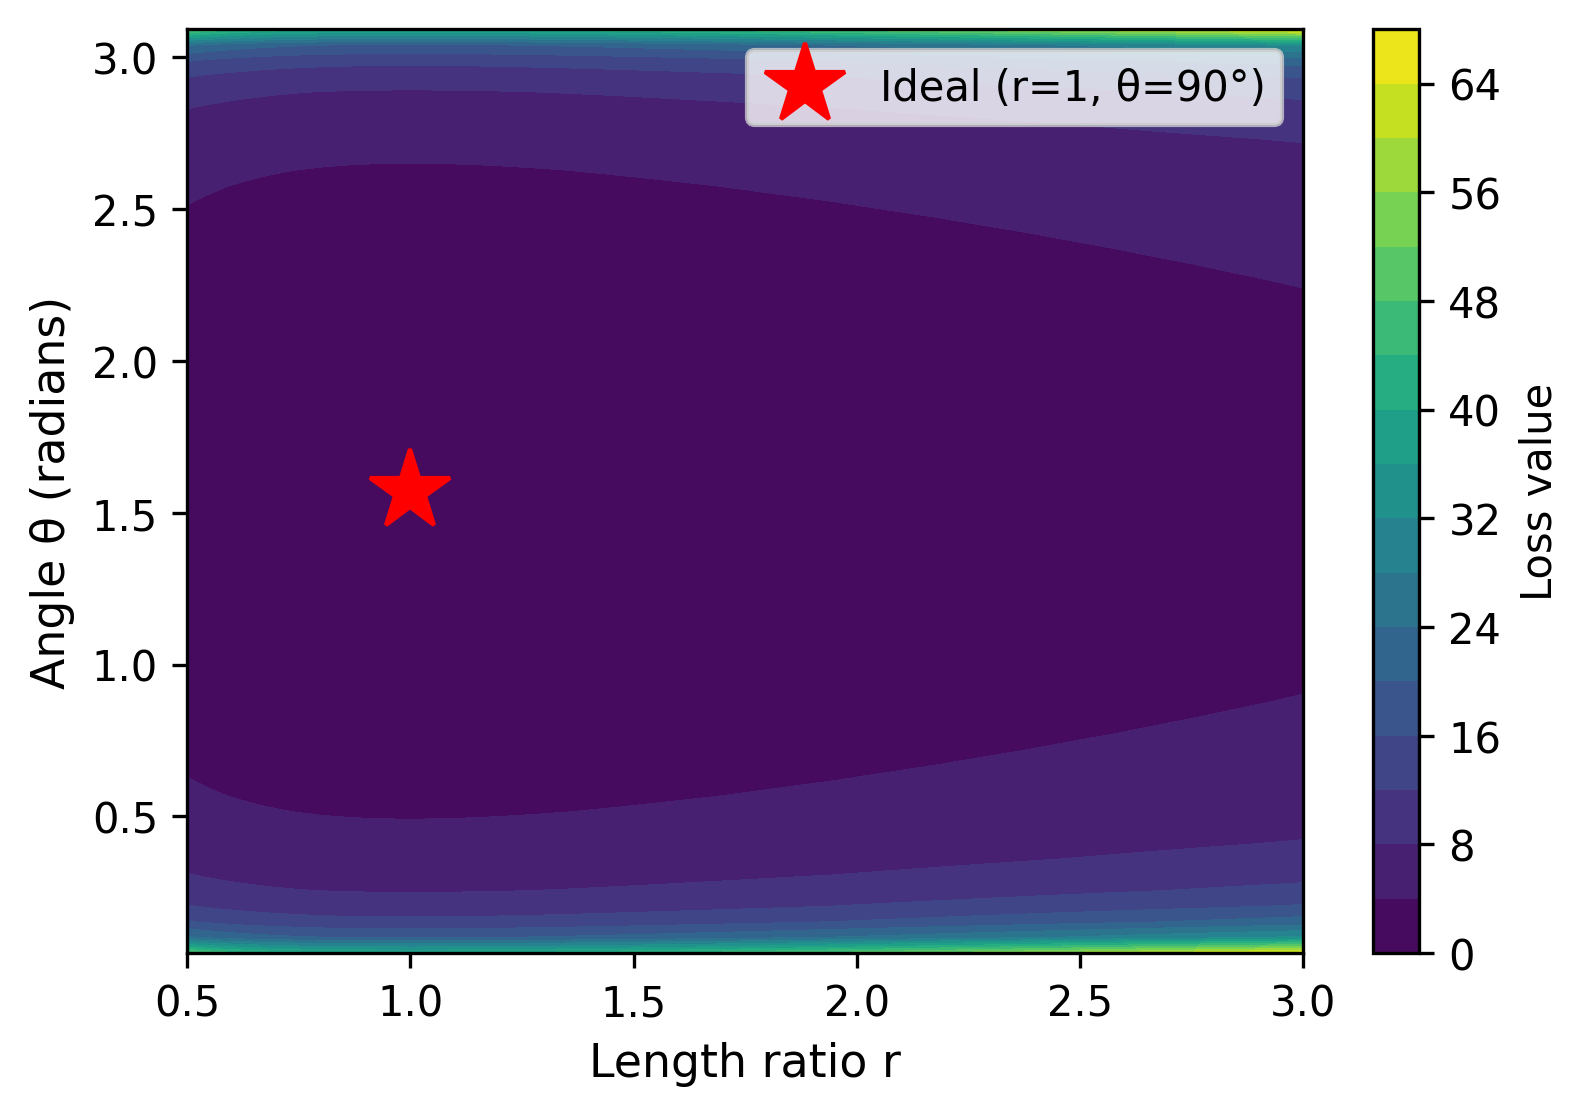
\includegraphics[width=0.48\linewidth]{../figures/loss_2d_condition_number.png} &
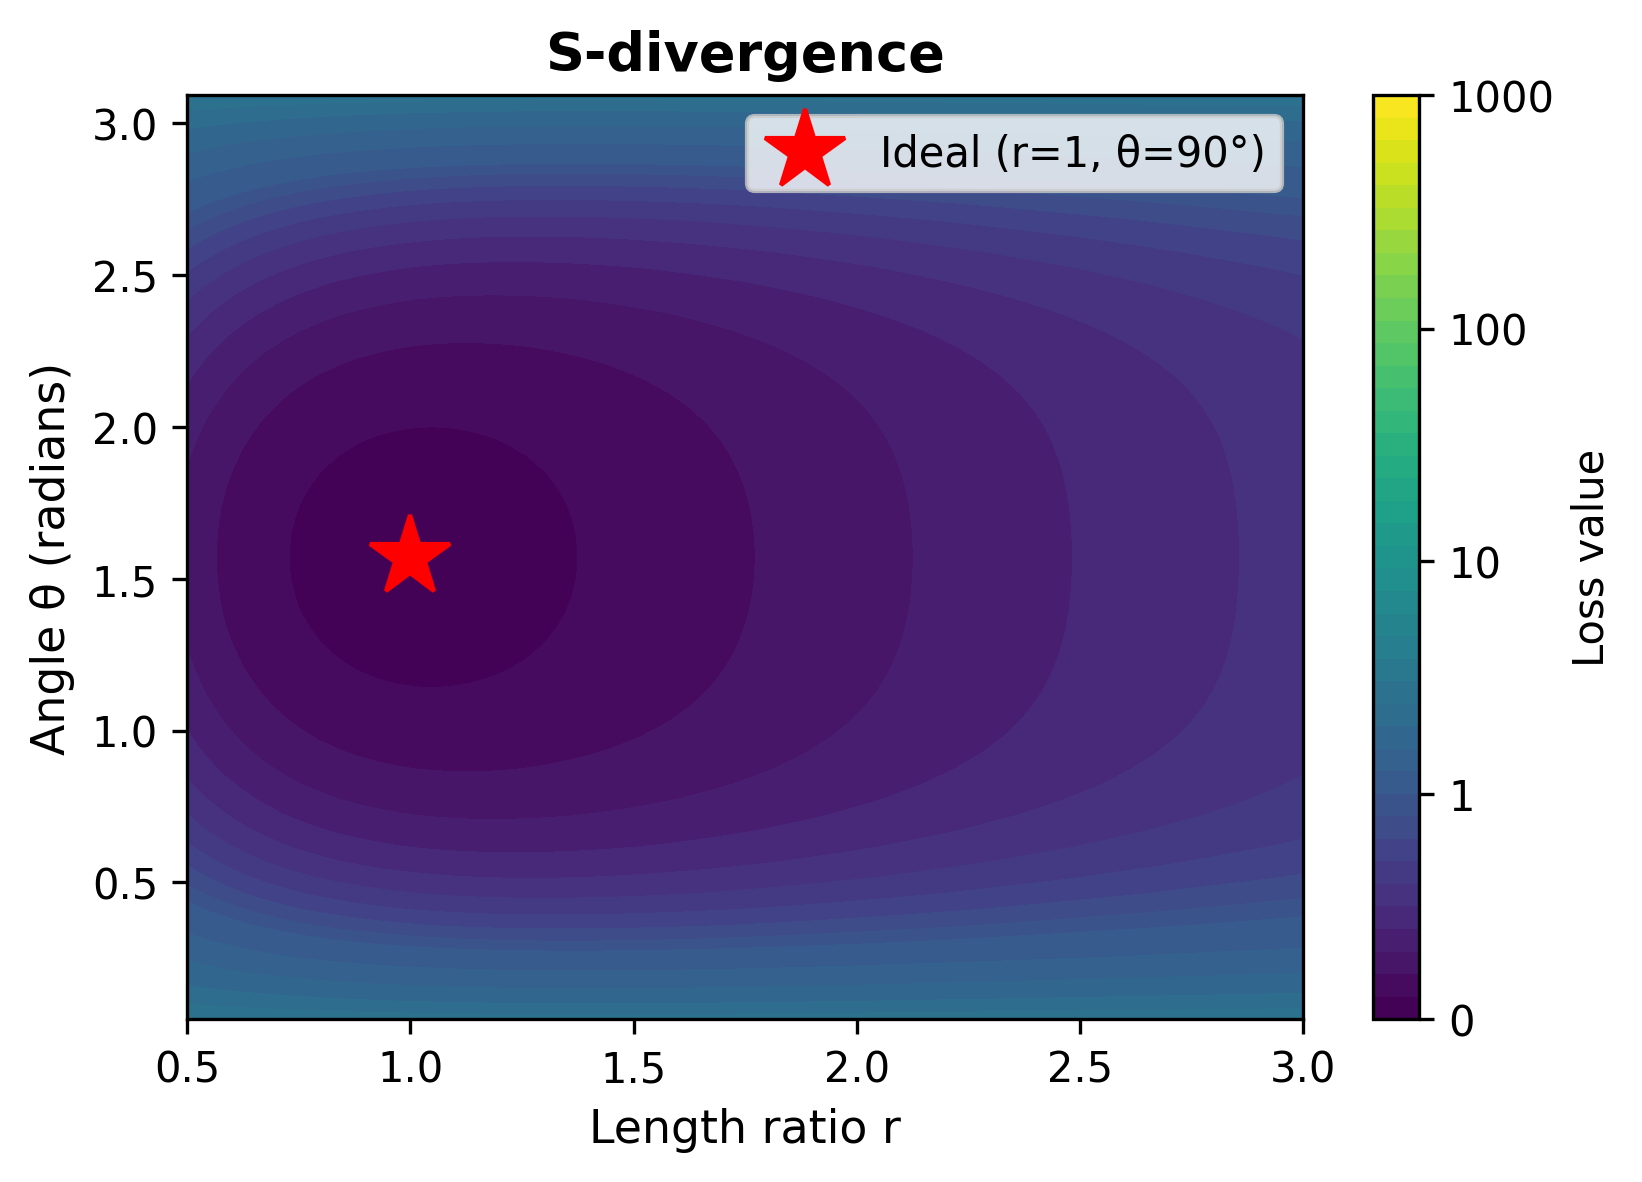
\includegraphics[width=0.48\linewidth]{../figures/loss_2d_s_divergence_identity.png} \\
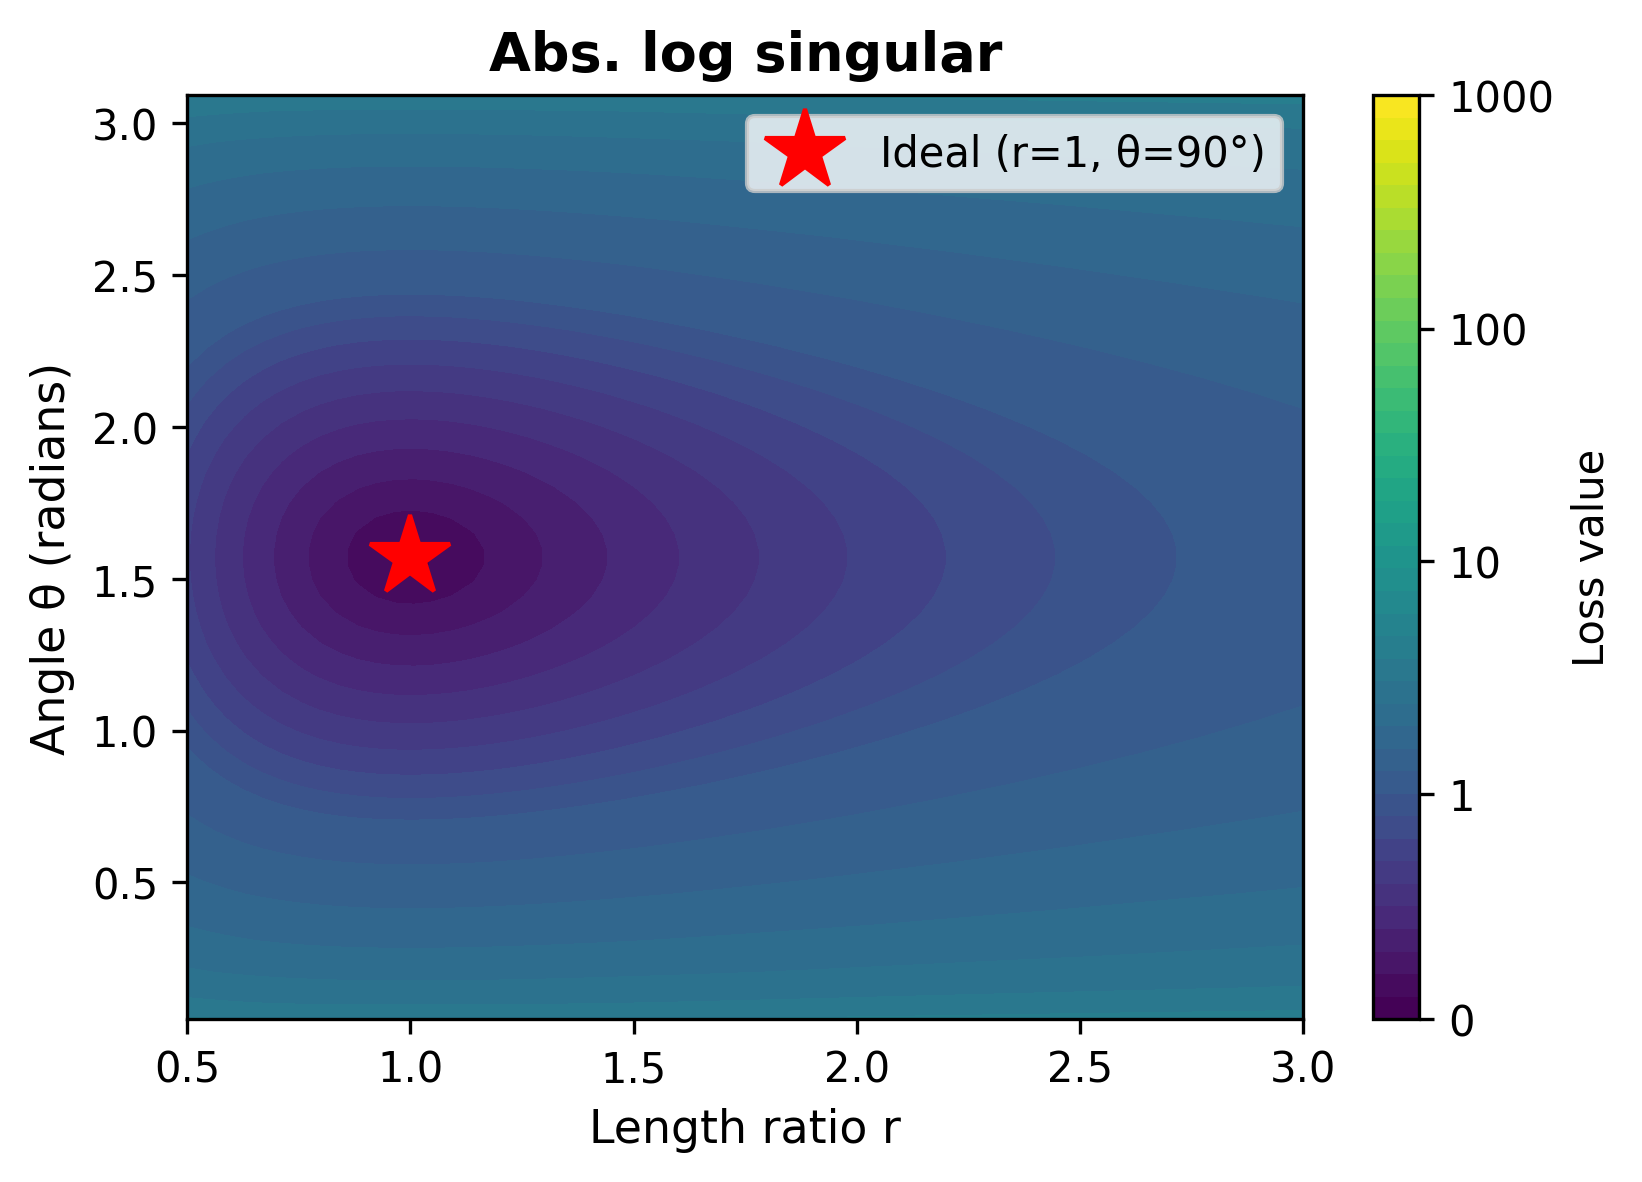
\includegraphics[width=0.48\linewidth]{../figures/loss_2d_absolute_log_singular_values.png} &
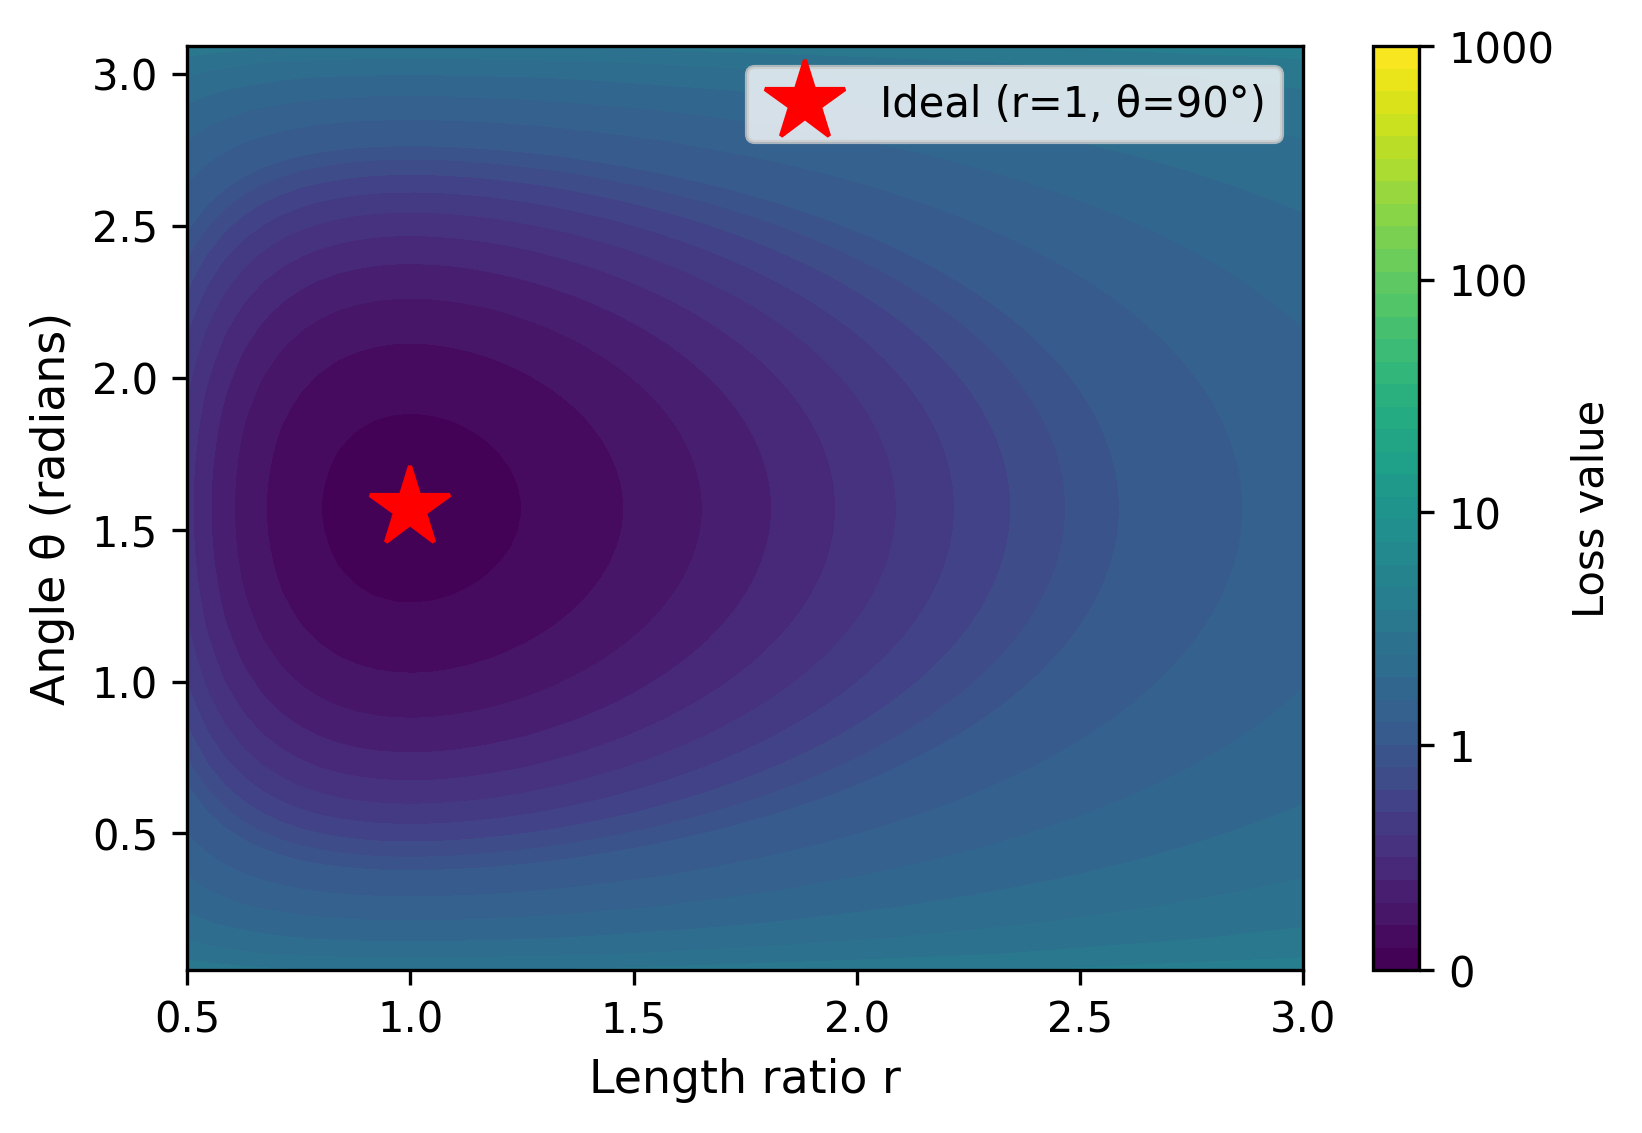
\includegraphics[width=0.48\linewidth]{../figures/loss_2d_normalized_logdet_volume.png} \\
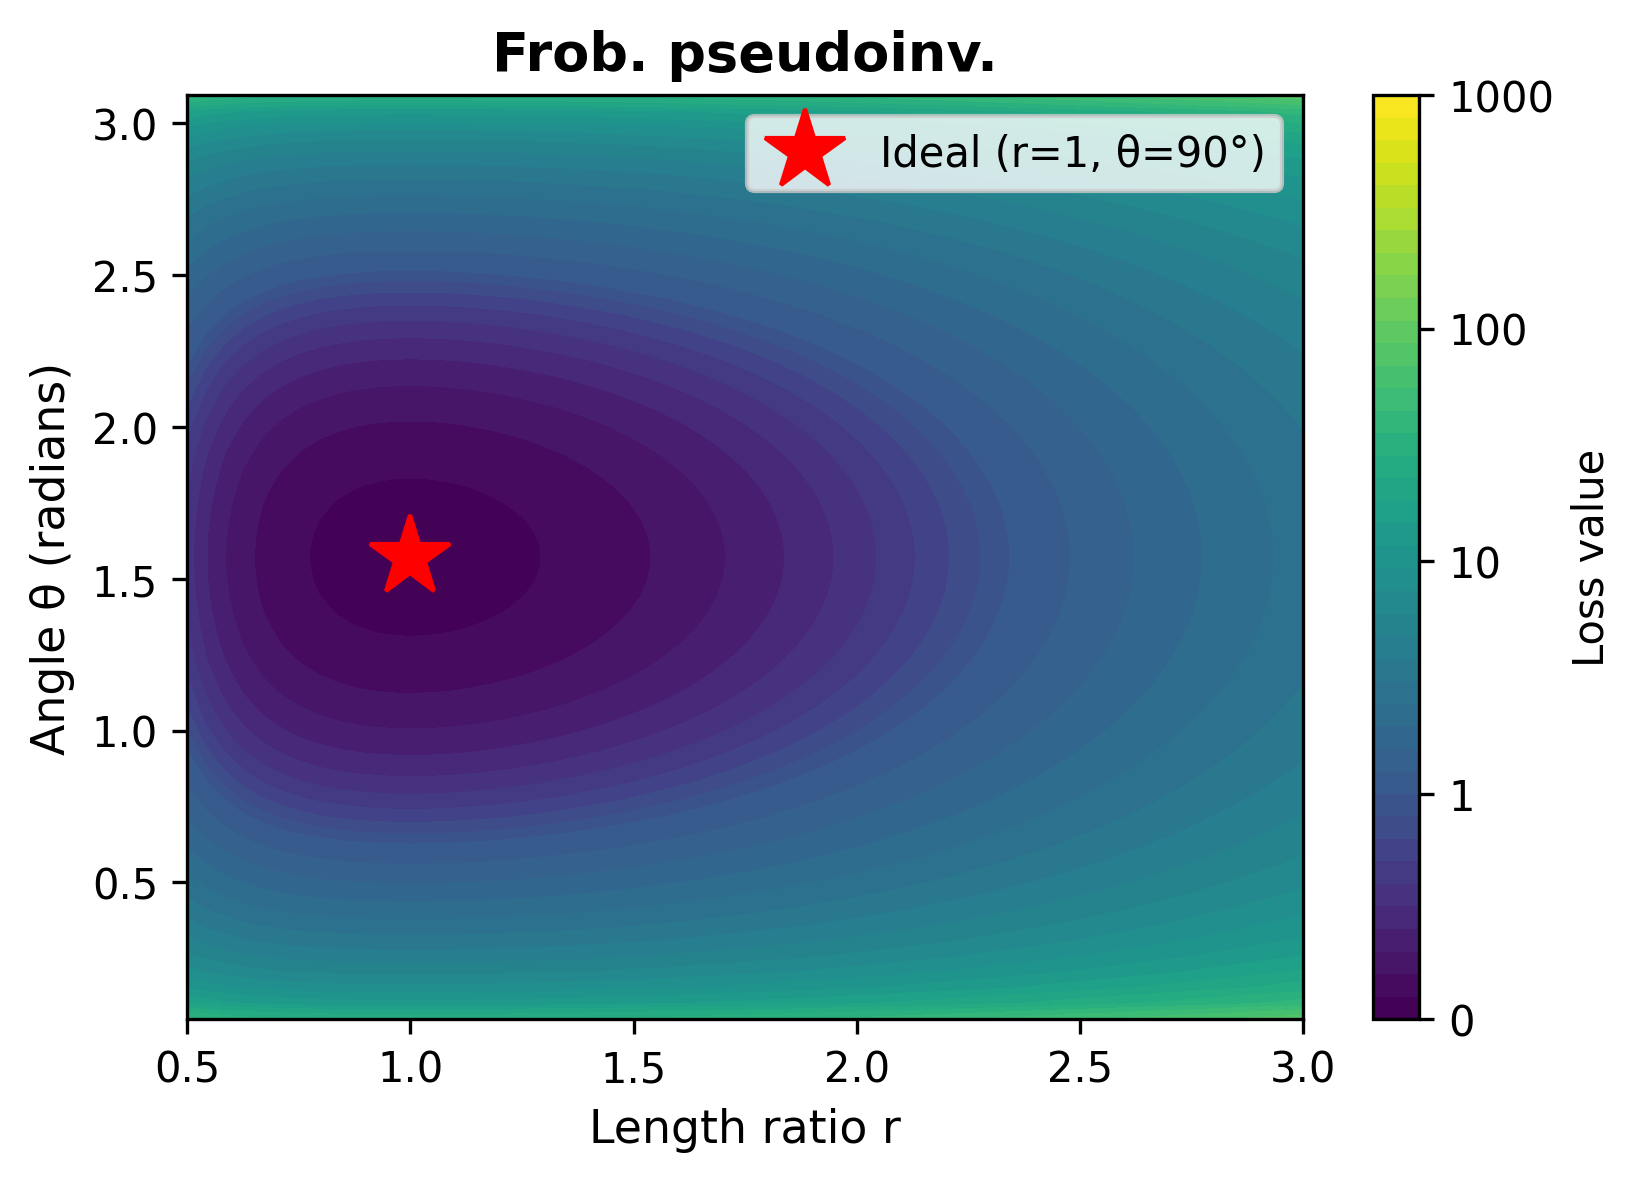
\includegraphics[width=0.48\linewidth]{../figures/loss_2d_frob_pseudoinverse.png} &
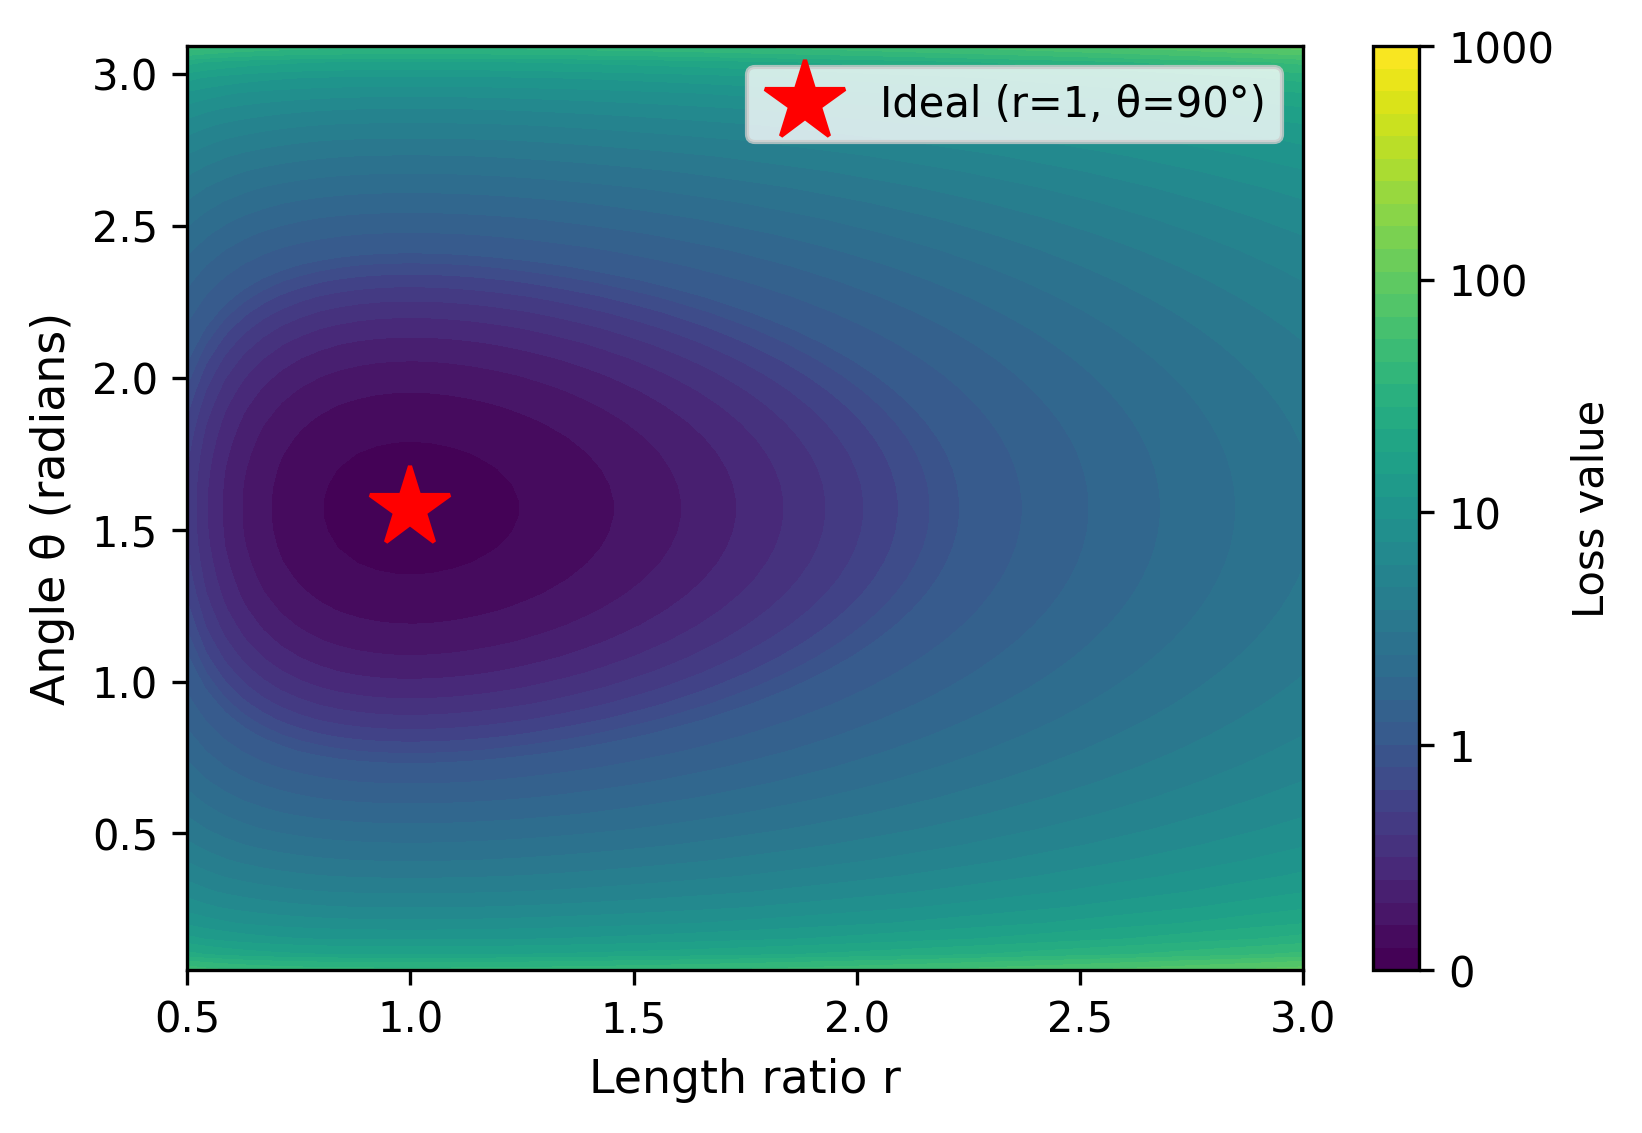
\includegraphics[width=0.48\linewidth]{../figures/loss_2d_gl_pseudoinverse.png}
\end{tabular}
\endgroup
\caption{$2 \times 2$ matrices.}
\label{fig:loss_landscapes}
\end{subfigure}\hfill
\begin{subfigure}[t]{0.49\textwidth}
\centering
\begingroup
\setlength{\tabcolsep}{1pt}
\begin{tabular}{@{}cc@{}}
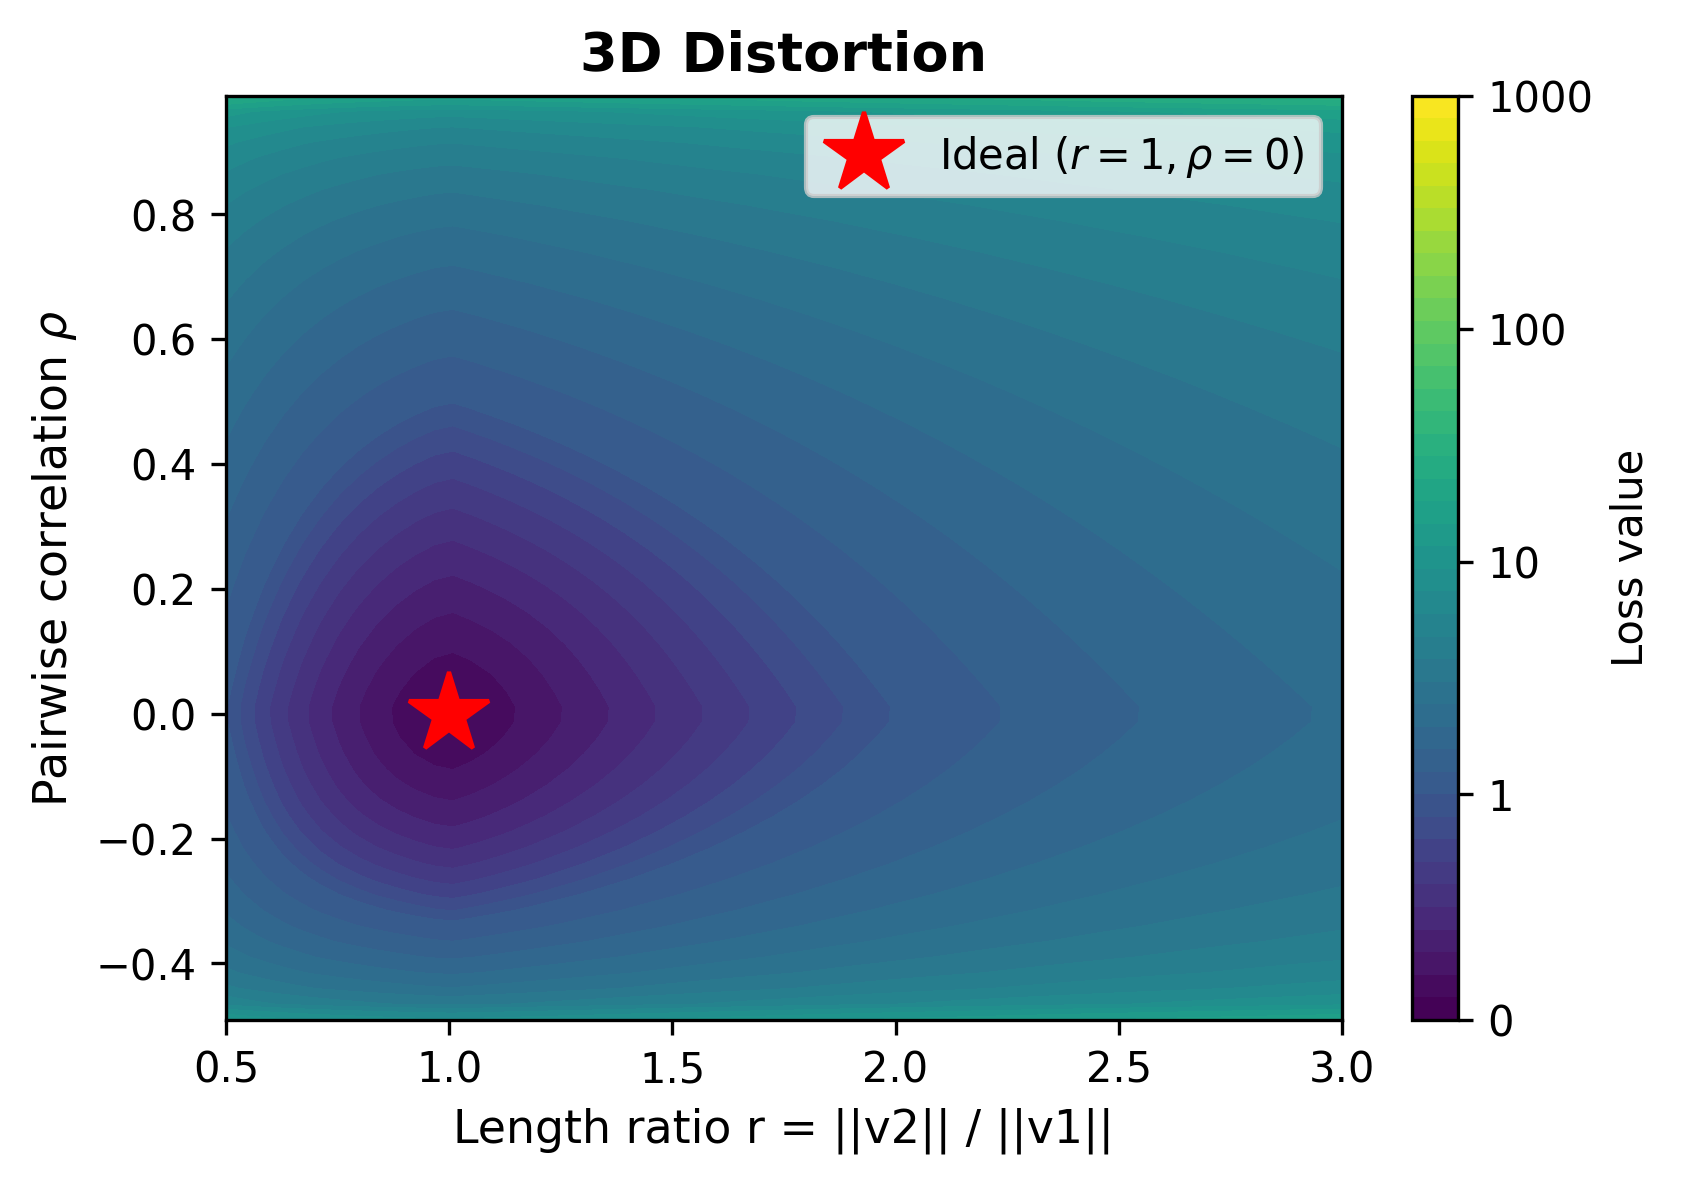
\includegraphics[width=0.48\linewidth]{../figures/loss_3d_equicorr_condition_number.png} &
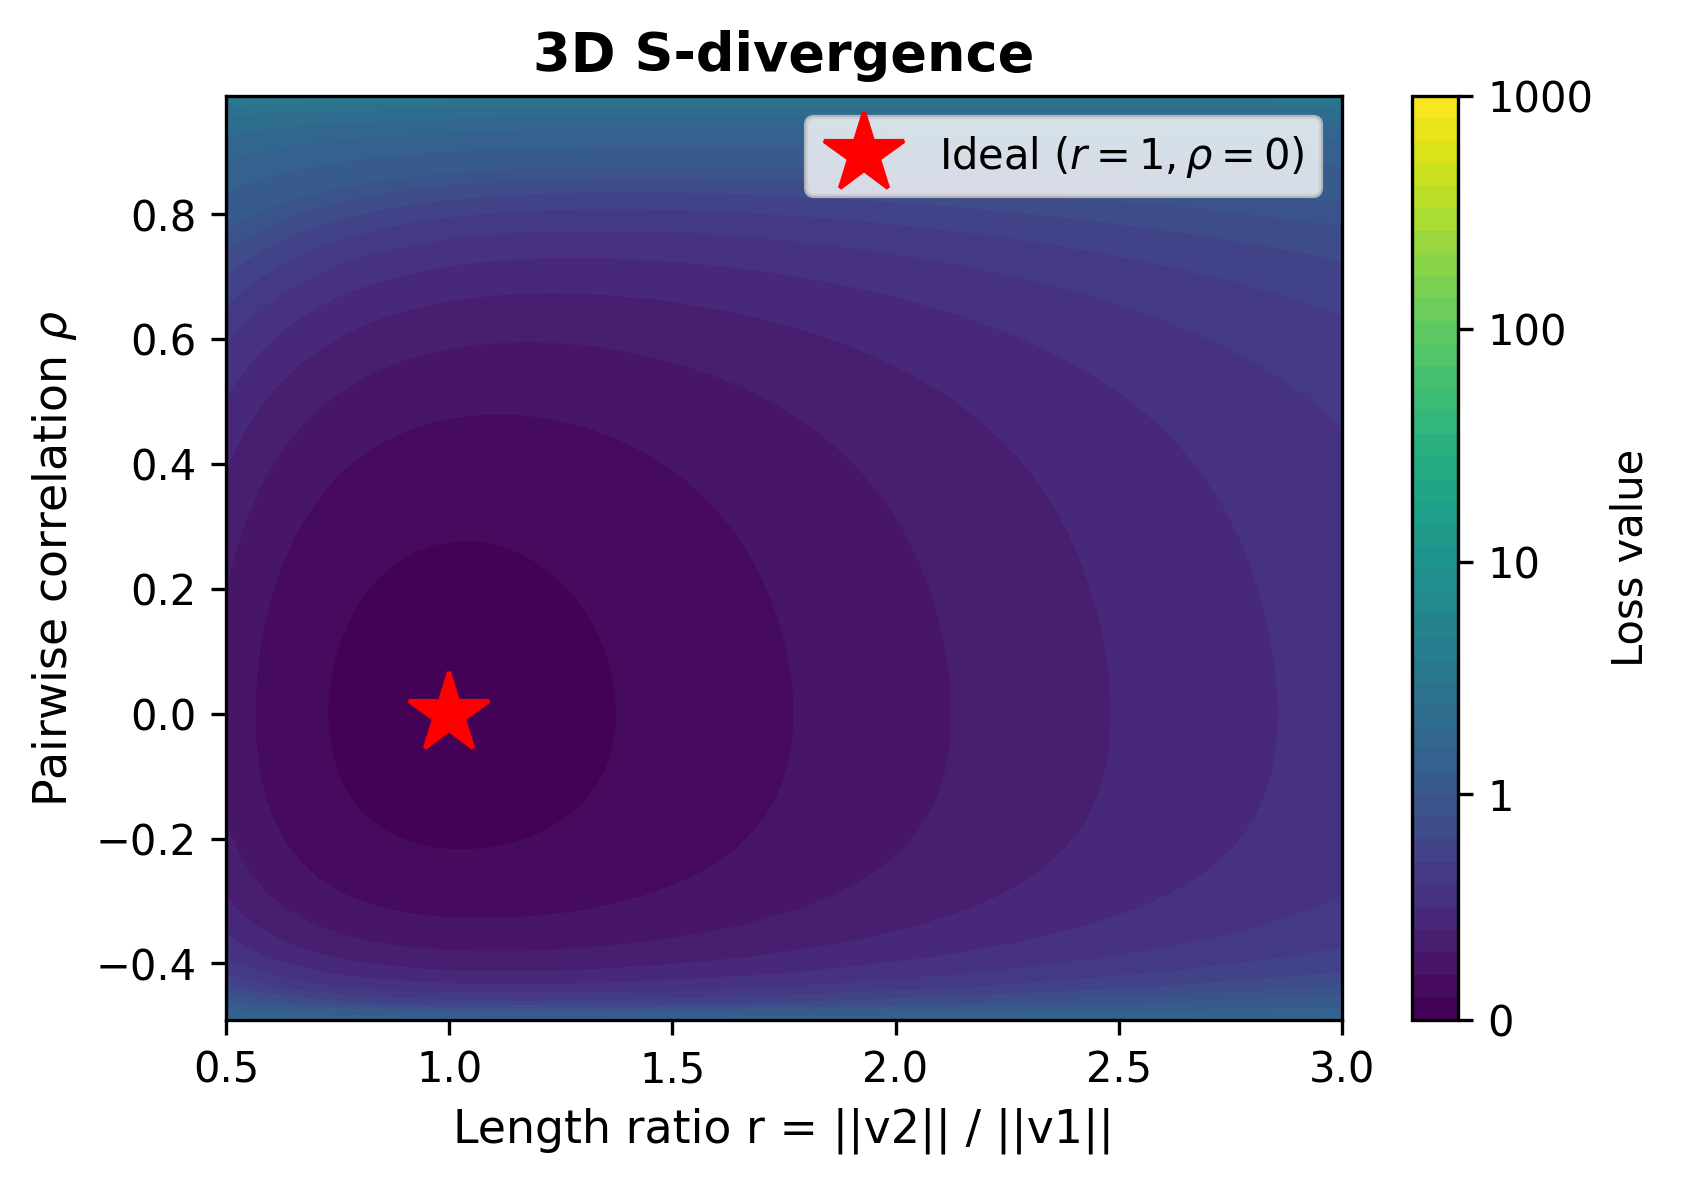
\includegraphics[width=0.48\linewidth]{../figures/loss_3d_equicorr_s_divergence_identity.png} \\
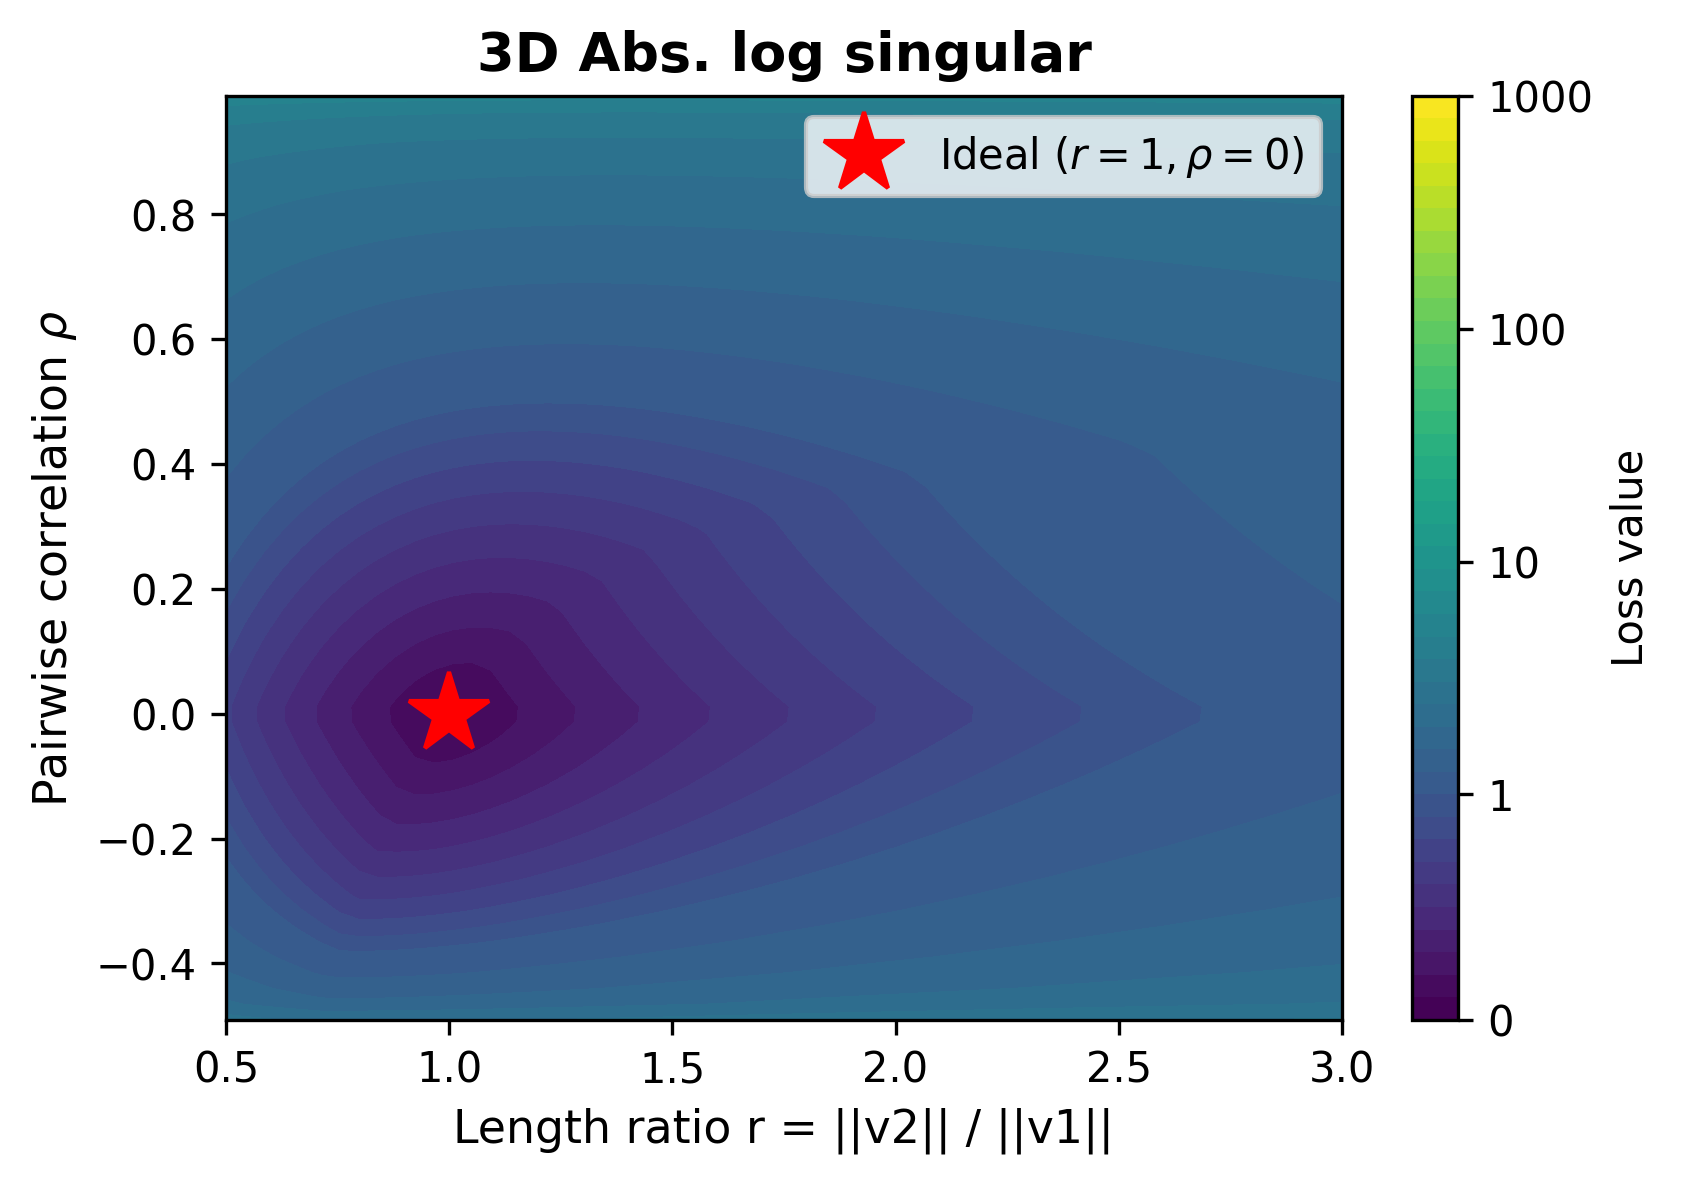
\includegraphics[width=0.48\linewidth]{../figures/loss_3d_equicorr_absolute_log_singular_values.png} &
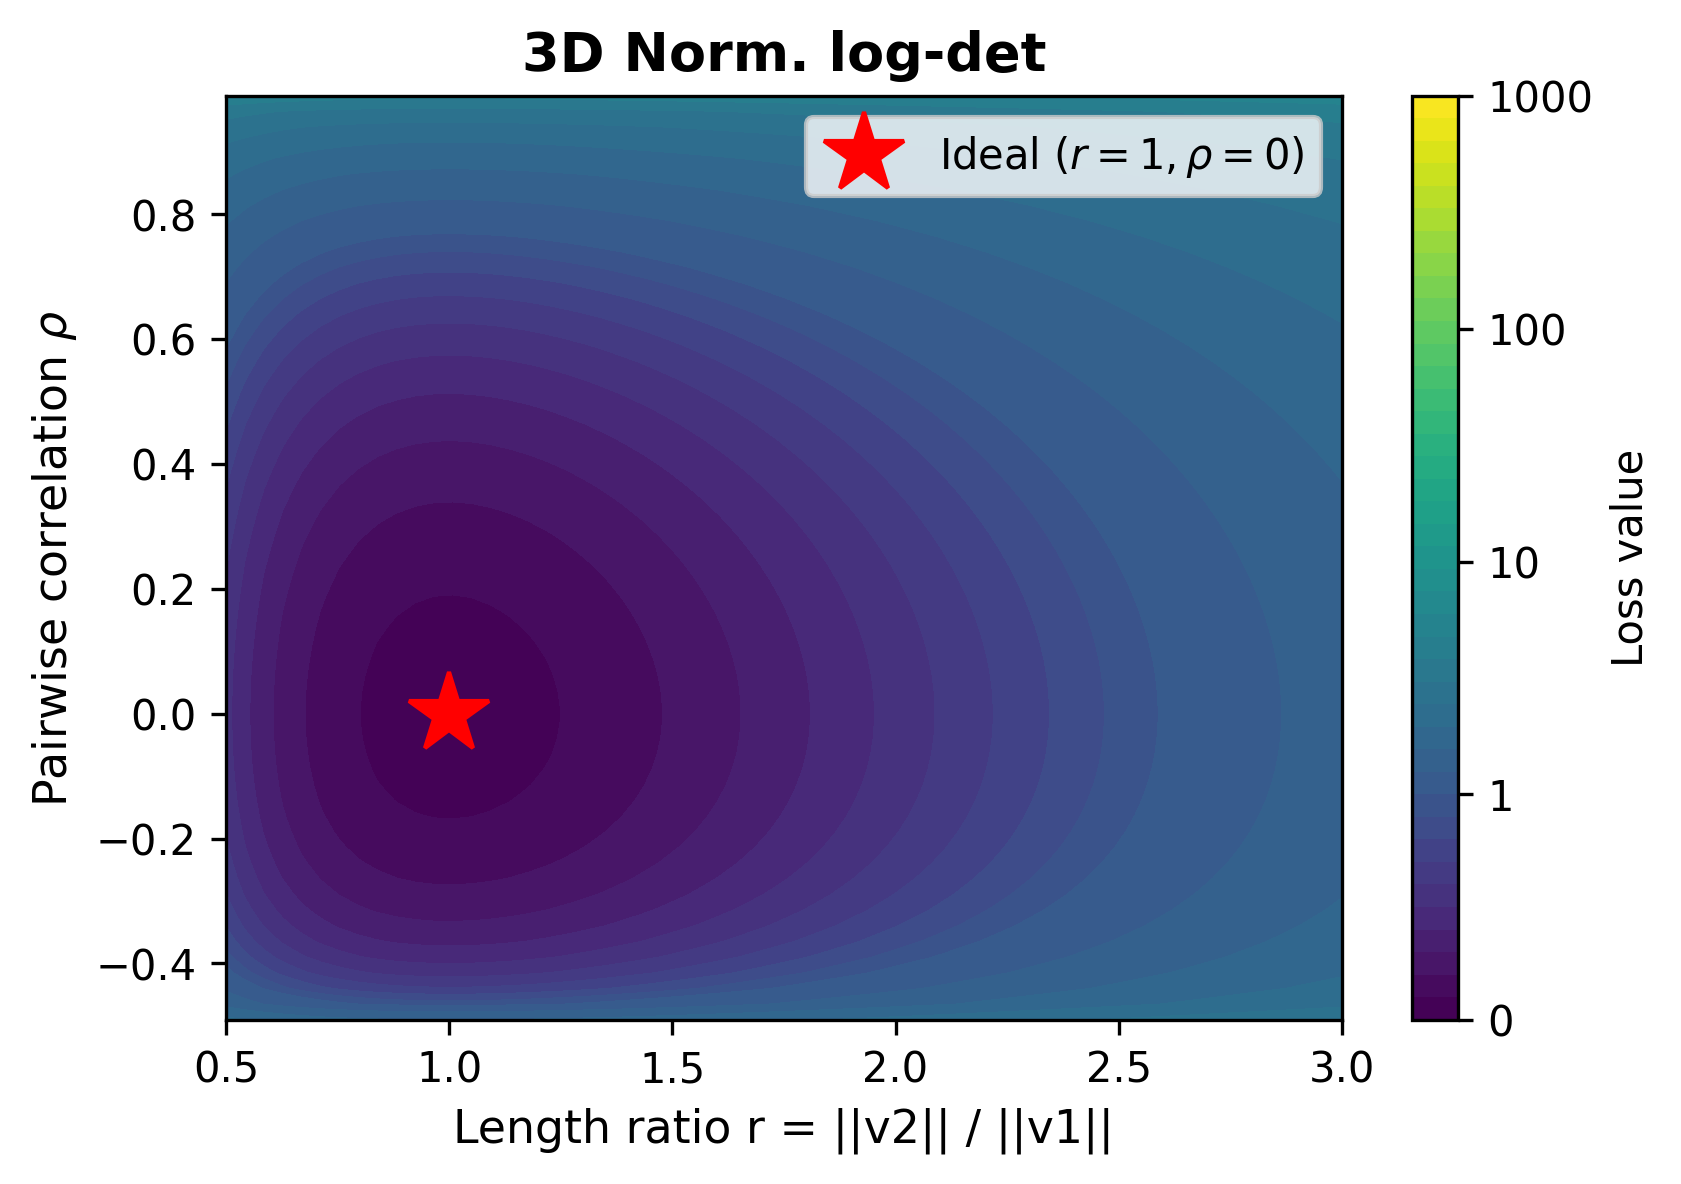
\includegraphics[width=0.48\linewidth]{../figures/loss_3d_equicorr_normalized_logdet_volume.png} \\
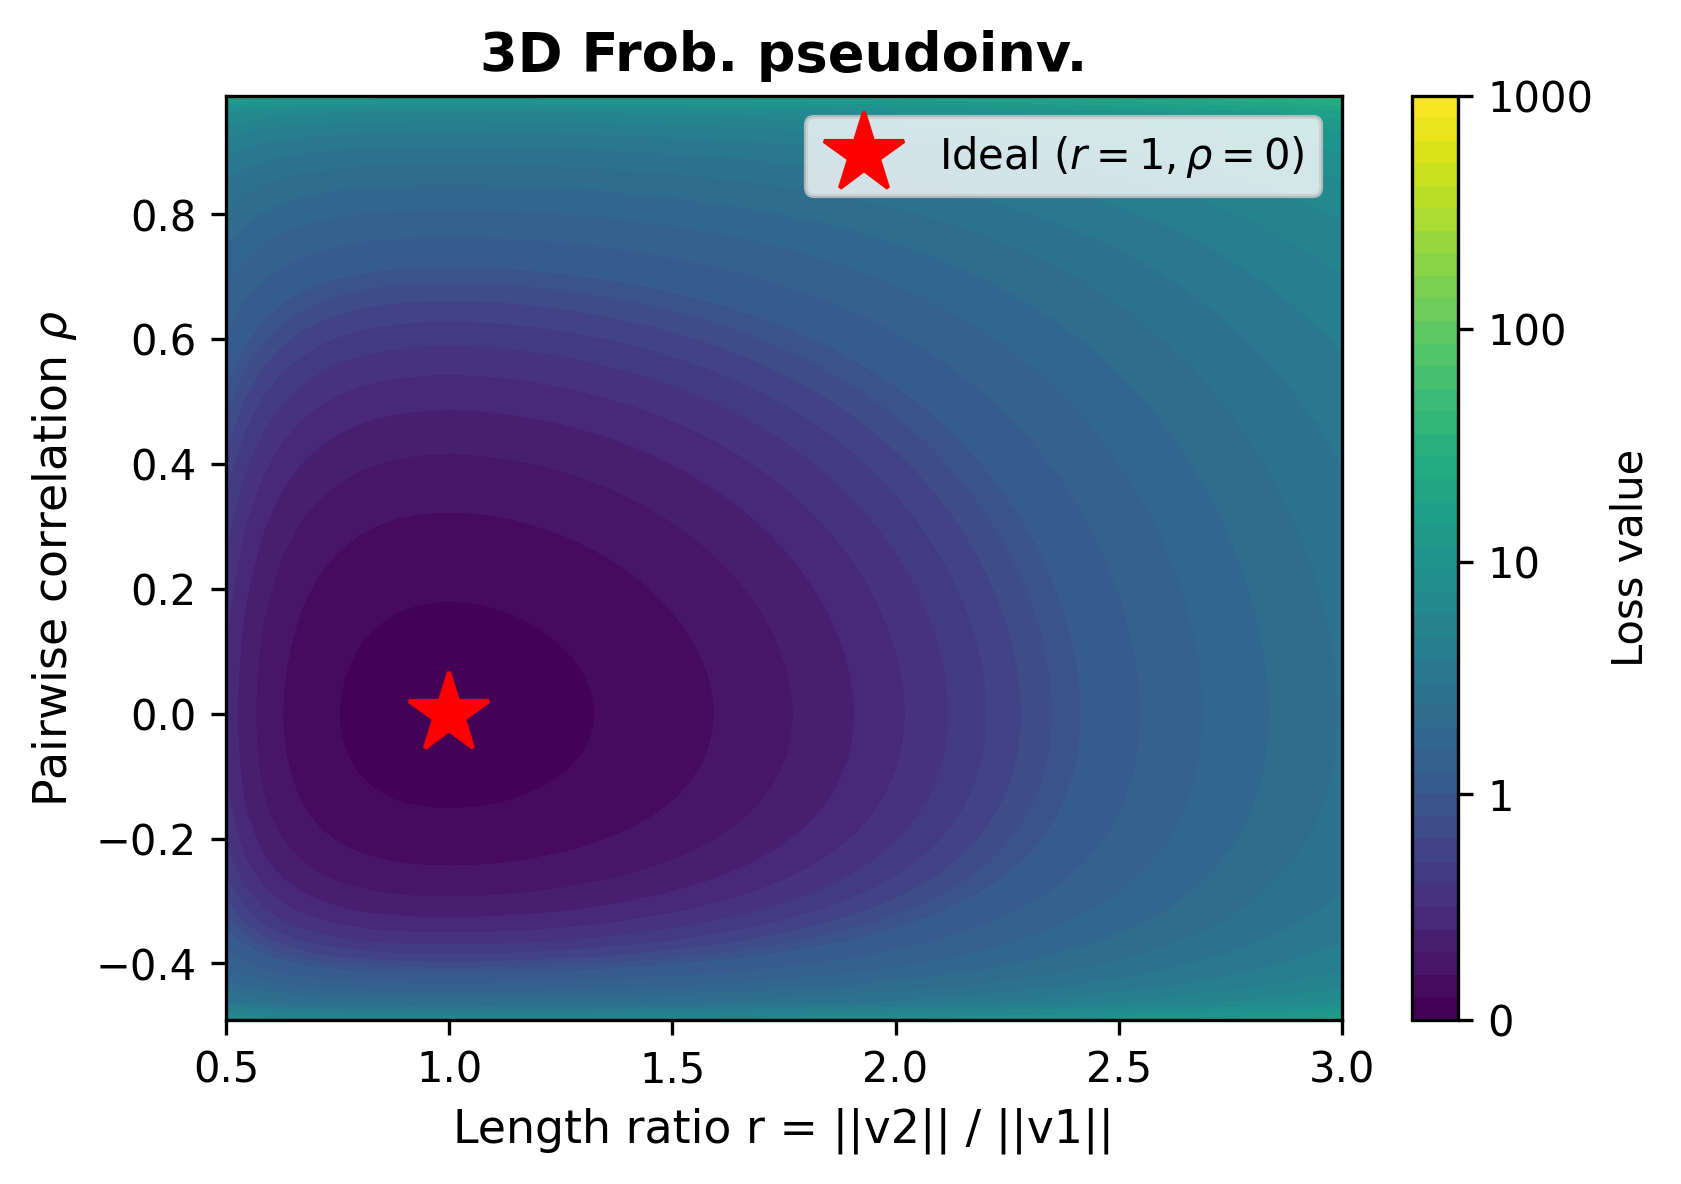
\includegraphics[width=0.48\linewidth]{../figures/loss_3d_equicorr_frob_pseudoinverse.png} &
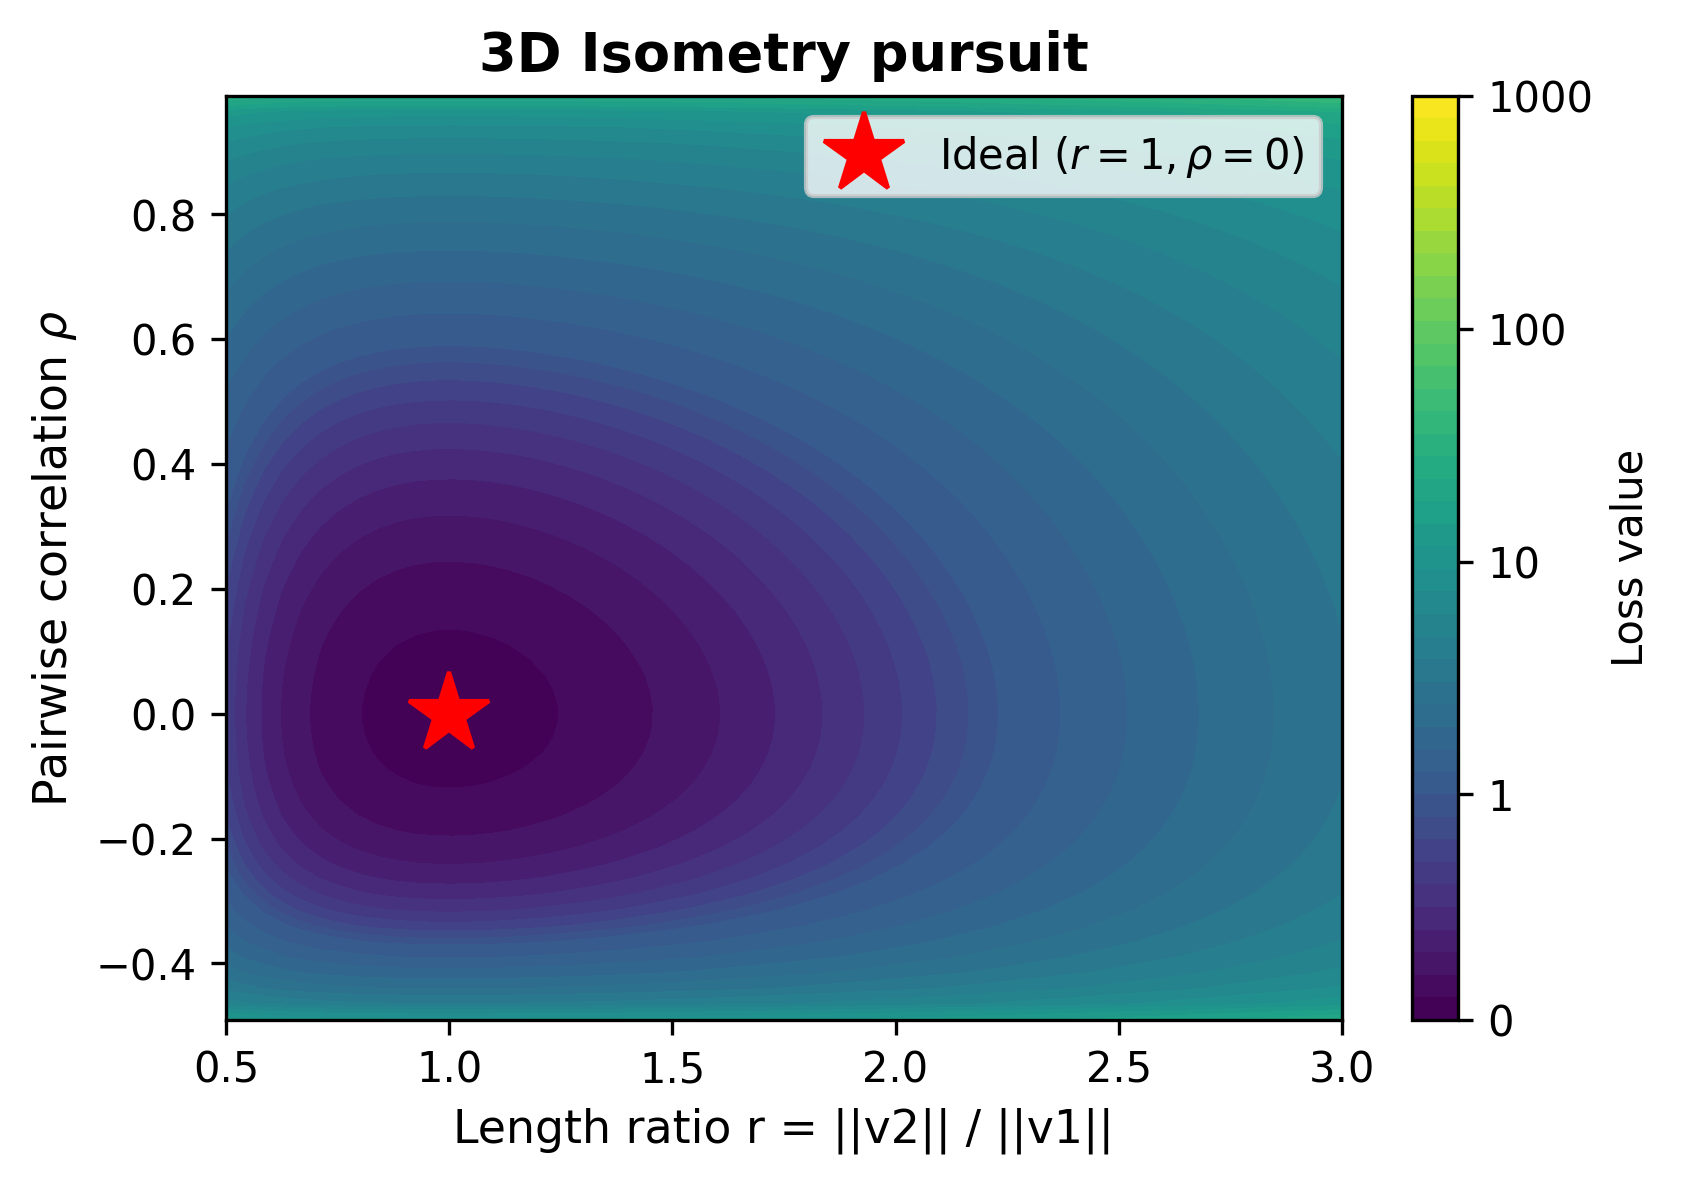
\includegraphics[width=0.48\linewidth]{../figures/loss_3d_equicorr_gl_pseudoinverse.png}
\end{tabular}
\endgroup
\caption{Equicorrelated $3 \times 3$ matrices.}
\label{fig:loss_3d_equicorr_landscapes}
\end{subfigure}
\caption{Loss function comparison. (a) Each landscape varies the length ratio
$r$ and angle $\theta$ between two column vectors. (b) Each matrix consists of
three vectors in $\mathbb R^3$ with lengths $(1,r,1)$ and common pairwise
correlation $\rho$; the horizontal axis varies
$r=\|v_2\|_2/\|v_1\|_2$ and the vertical axis varies $\rho$.
S-divergence and absolute log singular value are representative generic
spectral losses. The red star marks the ideal orthonormal setting:
$(r,\theta)=(1,\pi/2)$ in (a) and $(r,\rho)=(1,0)$ in (b).
See Table \ref{tab:loss_functions} for mathematical definitions.}
\end{figure}

% compares it with that produced by basis pursuit after normalization as in Section \ref{sec:normalization}.
% NOTE (Sam): Do we need proofs of maximized by orthonormal matrices and convex?
% Can we prove this is a norm?

We have established that there are losses $\ell$ that satisfy our conditions for a good loss function on square matrices $X \in \mathbb R^{D\times D}$.
However, the computational identification of such matrices is combinatorial in nature.
To avoid this, we reformulate the problem as a sparse convex optimization problem.
The Frobenius norm of the inverse has a natural relaxation to the high-dimensional setting in the form of basis pursuit.

\subsection{Isometry pursuit}

Isometry pursuit is the application of multitask basis pursuit to the normalized design matrix $w(X)$ to identify submatrices of $ X$ that are as orthonormal as possible.
Define the multitask basis pursuit penalty 
\begin{align}
\label{eq:bp}
\| \cdot \|_{1,2}: \mathbb R^{P \times D} &\to \mathbb R^+ \\ 
\beta &\mapsto  \sum_{p=1}^P  \|\beta_{p.}\|_2.
\end{align}
Given a matrix $Y \in \mathbb R^{D \times D}$, the multitask basis pursuit solutions are
\begin{align}
\label{prog:multitask_basis_pursuit}
\widehat {\mathcal {\beta}}_{MBP} (X, Y)  := \arg \min_{\beta \in \mathbb R^{P \times D}} \| \beta \|_{1,2} \; : \;Y =  X \beta.
\end{align}

The multitask basis pursuit solution is often not unique.
See \citet{Schneider2022-hi} for more details on uniqueness of basis pursuit solutions, for which the uniqueness condition is less strict than in the multitask case.
We therefore define
\begin{align}
\widehat \beta^{\ell_2}_{MLP} (X,Y) := \arg \min \|\beta\|_F : \beta \in \mathcal \beta_{MBP} (X, Y) .
\end{align}
By the strong convexity of the $\ell_2$ norm, $\widehat \beta^{\ell_2}_{MLP} (X,Y)$ is well defined.
% 
% Given a design matrix $X$, there exists a response variable $y$ such that basis pursuit admits a non-unique solution if and only if the rowspan of the design matrix $X$ contains a sufficient codimension edge of the $p$ dimensional hypercube \citep{Schneider2022-hi}.
% For multitask basis pursuit non-unique solutions may occur even when this condition is satisfied.

This implicit regularization assumption is reasonable.
% Mishkin2023-yt is broken
For example, in \citet{Tibshirani2012-vw} the implicit selection of the minimum $\ell_2$ norm solution among the lasso solutions was proven for the Least Angle Regression Selection (LARS) algorithm for solving the lasso, while \citet{Mishkin2022-yf}  assumes that the group lasso solution is in fact min-norm prior to subsequent theoretical analyses.
Empirically, the Splitting Conic Solver type method (which is itself a variant of the Alternating Direction Method of Multilpliers) \citep{O-Donoghue2013-wf} stably estimates the min-norm solution when initialized at $0$, but besides a brief exploration in Section \ref{sec:deep_dive} we leave theoretical and experimental proof of this feature of the feature our optimization approach for future work, and instead make the ability of our optimizer to obtain the min-norm solution an assumption of our eventual proposition.

Isometry pursuit is then given by
\begin{align}
\label{prog:isometry_pursuit}
\widehat \beta ( X) := \widehat \beta_{MBP}^{\ell_2} ( w(X), I_D )
\end{align}
where $I_D$ is the $D$ dimensional identity matrix and recovered functions are the indices of the dictionary elements with non-zero coefficients.
That is, they are given by $S(\beta)$ where
\begin{align}
S: \mathbb{R}^{P \times D} &\to \binom{[P]}{D} \\
\beta &\mapsto \left\{ p \in [P] :  \|\beta_{p.}\| > 0 \right\}.
\end{align}
\begin{algorithm}[H]
\caption{\isometrypursuit(Matrix ${X} \in \mathbb{R}^{D \times P}$)}
\begin{algorithmic}[1]
\STATE {Normalize} $X' = w({X})$
\STATE {Optimize} $\widehat \beta = \widehat \beta_{MBP}^{\ell_2} (X', I_D)$
\STATE {\bf Output} $\widehat{S} = S (\widehat \beta)$
\end{algorithmic}
\end{algorithm}

\subsection{Theory}

The intuition behind our application of multitask basis pursuit is that submatrices consisting of vectors which are closer to 1 in length and more orthogonal will have smaller loss.
A key theoretical assertion is that \isometrypursuit~ is invariant to choice of basis for $ X$.
\begin{proposition}
\label{prop:basis_pursuit_selection_invariance}
Let $U \in \mathbb R^{D \times D}$ be orthonormal.
Then $S(\widehat \beta  (U  X)) = S(\widehat \beta ( X))$.
\end{proposition}
This proposition establishes the basis-independence of Isometry Pursuit and that we may replace $I_D$ in the constraint by any orthonormal $D \times D$ matrix.
It is also essential for showing the following main theoretical result.

When a rank $D$ orthonormal column-submatrix $X_{.S}$ exists, the output of Program \ref{prog:isometry_pursuit} will contain $S$.
\begin{proposition}
Let $X \in \mathbb R^{D \times P}$ have a rank $D$ orthonormal column submatrix $X_{.S}$.
Then $S \subseteq \widehat \beta ( X)$.
\label{prop:unitary_selection}
\end{proposition}

Proofs of these propositions are given in Section \ref{sec:proofs}, with corresponding experimental results in Section \ref{sec:experiments}.
The proof mostly relies on the KKT conditions \citep{Hastie2015-qa} being used to verify that an isometric subset yields a corresponding basis pursuit solution for an appropriate normalized matrix.
This is a formalization of our intuition that longer and more orthogonal vectors will minimize loss.
We then apply a simple argument to show that the $\ell_2$ minimizing solution is the least sparse solution, which means that it contains the isometry solution, should it exist.

\subsection{Two-stage isometry pursuit}

Proposition \ref{prop:unitary_selection} suggests the following algorithm, which first uses the convex \isometrypursuit~ algorithm to prune the $P$ candidate features and then applies brute search upon the reduced feature set.
The proposition says that this approach is guaranteed to select an isometric submatrix should one exist.
The two-stage approach is standard in the Lasso literature \citep{Meinshausen2007-ey, Hesterberg2008-iy, Koelle2022-ju}, and Proposition \ref{prop:unitary_selection} justifies it in our application.
Bruckmeier et al.\ also use a convex relaxation to restrict subsequent discrete search \citep{Bruckmeier2023-cube}.
This method forms our practical isometry estimator, the core advantage of which over purely brute search is a substantially improved computational complexity.

\begin{algorithm}[H]
\caption{\tsip(Matrix ${X} \in \mathbb{R}^{D \times P}$)}
\begin{algorithmic}[1]
\STATE $\widehat{S}_{IP} = \text{\isometrypursuit}( X)$
\STATE $\widehat{S} = \text {\brute}({X}_{.\widehat{S}_{IP}}, \ell)$
\STATE {\bf Output} $\widehat{S}$
\end{algorithmic}
\end{algorithm}

\subsection{Non-uniqueness}

The isometric solution is optimum among cardinality $D$ solutions.
\begin{proposition}
\label{prop:D_min}
$\ell (X_S) = D , |S| = D \Leftrightarrow X_S X_S^T = I_D$
\end{proposition}
However, there exist Isometry Pursuit solutions of minimum norm that are not isometries.
For example, \textit{Mercedes-Benz frame} matrix $X$ achieves minimium norm.
\begin{example}
    Let $D = 2, P = 3$.
\label{prop:the_benzito}
Let 
$X_{S} = \begin{bmatrix}
0 & \frac{\sqrt{3}}{2}  &  - \frac{\sqrt{3}}{2}\\
1 & -\frac{1}{2} & -\frac{1}{2} 
\end{bmatrix},
    \beta = 
    \begin{bmatrix}
    0 & \frac{2}{3} \\
    \frac{1}{\sqrt{3}}  & - \frac{1}{3} \\
    - \frac{1}{\sqrt{3}} & - \frac{1}{3}
    \end{bmatrix}$
Then $X \beta = I_D$ and $\|\beta\|_{1,2} = \frac{2}{3} + \frac{2}{3} + \frac{2}{3} = 2 = D$.
Since the identity matrix is a solution regardless of $X_{-S}$, this is a non-isometric minimum loss solution.
\end{example}

The upshot of this example is that \isometrypursuit~ can select solutions that are relatively non-isometric.
The Mercedes-Benz frame is an example of a tight frame - a frame whose non-zero singular values are equal.
While there are non-tight frames that have minimizing solutions, we do not here resolve whether there exist tight frames with unit norm columns that have minimum norm solutions.

\subsection{Computation complexity}

\isometrypursuit~ is more computationally efficient than \brute~ search for the minimizer of $\ell$.
Interestingly, their asymptotic per-iteration complexities are the same.
\begin{proposition}
    \label{prop:computational_complexity}
    The computational complexity $C_\ell$ of \ref{eq:gt_loss} is $ O(D^2P)$.
\end{proposition}
The above proposition follows immediately from the computational complexity of singular value decomposition \citep{Liang2016-qb}.
The per-iteration complexity of \isometrypursuit~ is also limited by the computational complexity of singular value decomposition, albeit in the more intricate manner described in Section \ref{proof:computational_complexity}.
\begin{proposition}
\label{prop:computational_complexity}
The computational complexity of each step of Isometry Pursuit is $O(D^2P)$.
\end{proposition}

The difference therefore lies in the relation of the number of iterations required to achieve a given error tolerance with \isometrypursuit~ and \brute.
To optimize, we use the SCS interior point solver \citep{ocpb:16} from CVXPY \citep{diamond2016cvxpy, agrawal2018rewriting}, which is able to push sparse values arbitrarily close to 0 \citep{cvxpy_sparse_solution}.
SCS (aka ADMM) has asymptotic (in error) accuracy $\epsilon < O(\frac{1}{\mathcal S})$, where $\mathcal S$ is the number of iterations \citep{He2012-fi}.
This means that the number of iterations required to achieve a given error tolerance scales inversely with the desired level of accuracy.
We examine the effect of iteration number on the convergence to a sparse solution in Section \ref{sec:experiments}.

\section{Experiments}
\label{sec:experiments}

Say you are hosting a dinner party, and wish to select a balanced set of wines for drinking and flowers for decoration.
We compare four fixed-cardinality search pipelines: forward greedy and backward greedy initialization, each applied either to the full dictionary or after restriction by \isometrypursuit.
Each initializer is followed by one-for-one exchange search, which repeatedly replaces one selected column with one unselected column whenever the exchange reduces the loss.
This is a fixed-cardinality form of forward-backward greedy search \citep{pmlr-v32-liub14}; full algorithmic definitions are given in Section~\ref{sec:algorithms}.
We evaluate these pipelines on the Iris and Wine datasets \citep{misc_iris_53, misc_wine_109, scikit-learn}.
This has an intuitive interpretation as selecting diverse elements that reflects the peculiar structure of the diversification problem.
Features like \textit{petal width} are rows in $X$.
Thus, in diversification, $P = n$.
Due to differences in scales between features, these are first standardized.
For the Wine dataset, exhaustive \brute~ search is prohibitive in $D=13$, and so we compare practical discrete searches after random downsampling of candidate columns.

\begin{figure}[t]
    \centering
    \begin{subfigure}[t]{0.49\textwidth}
        \centering
        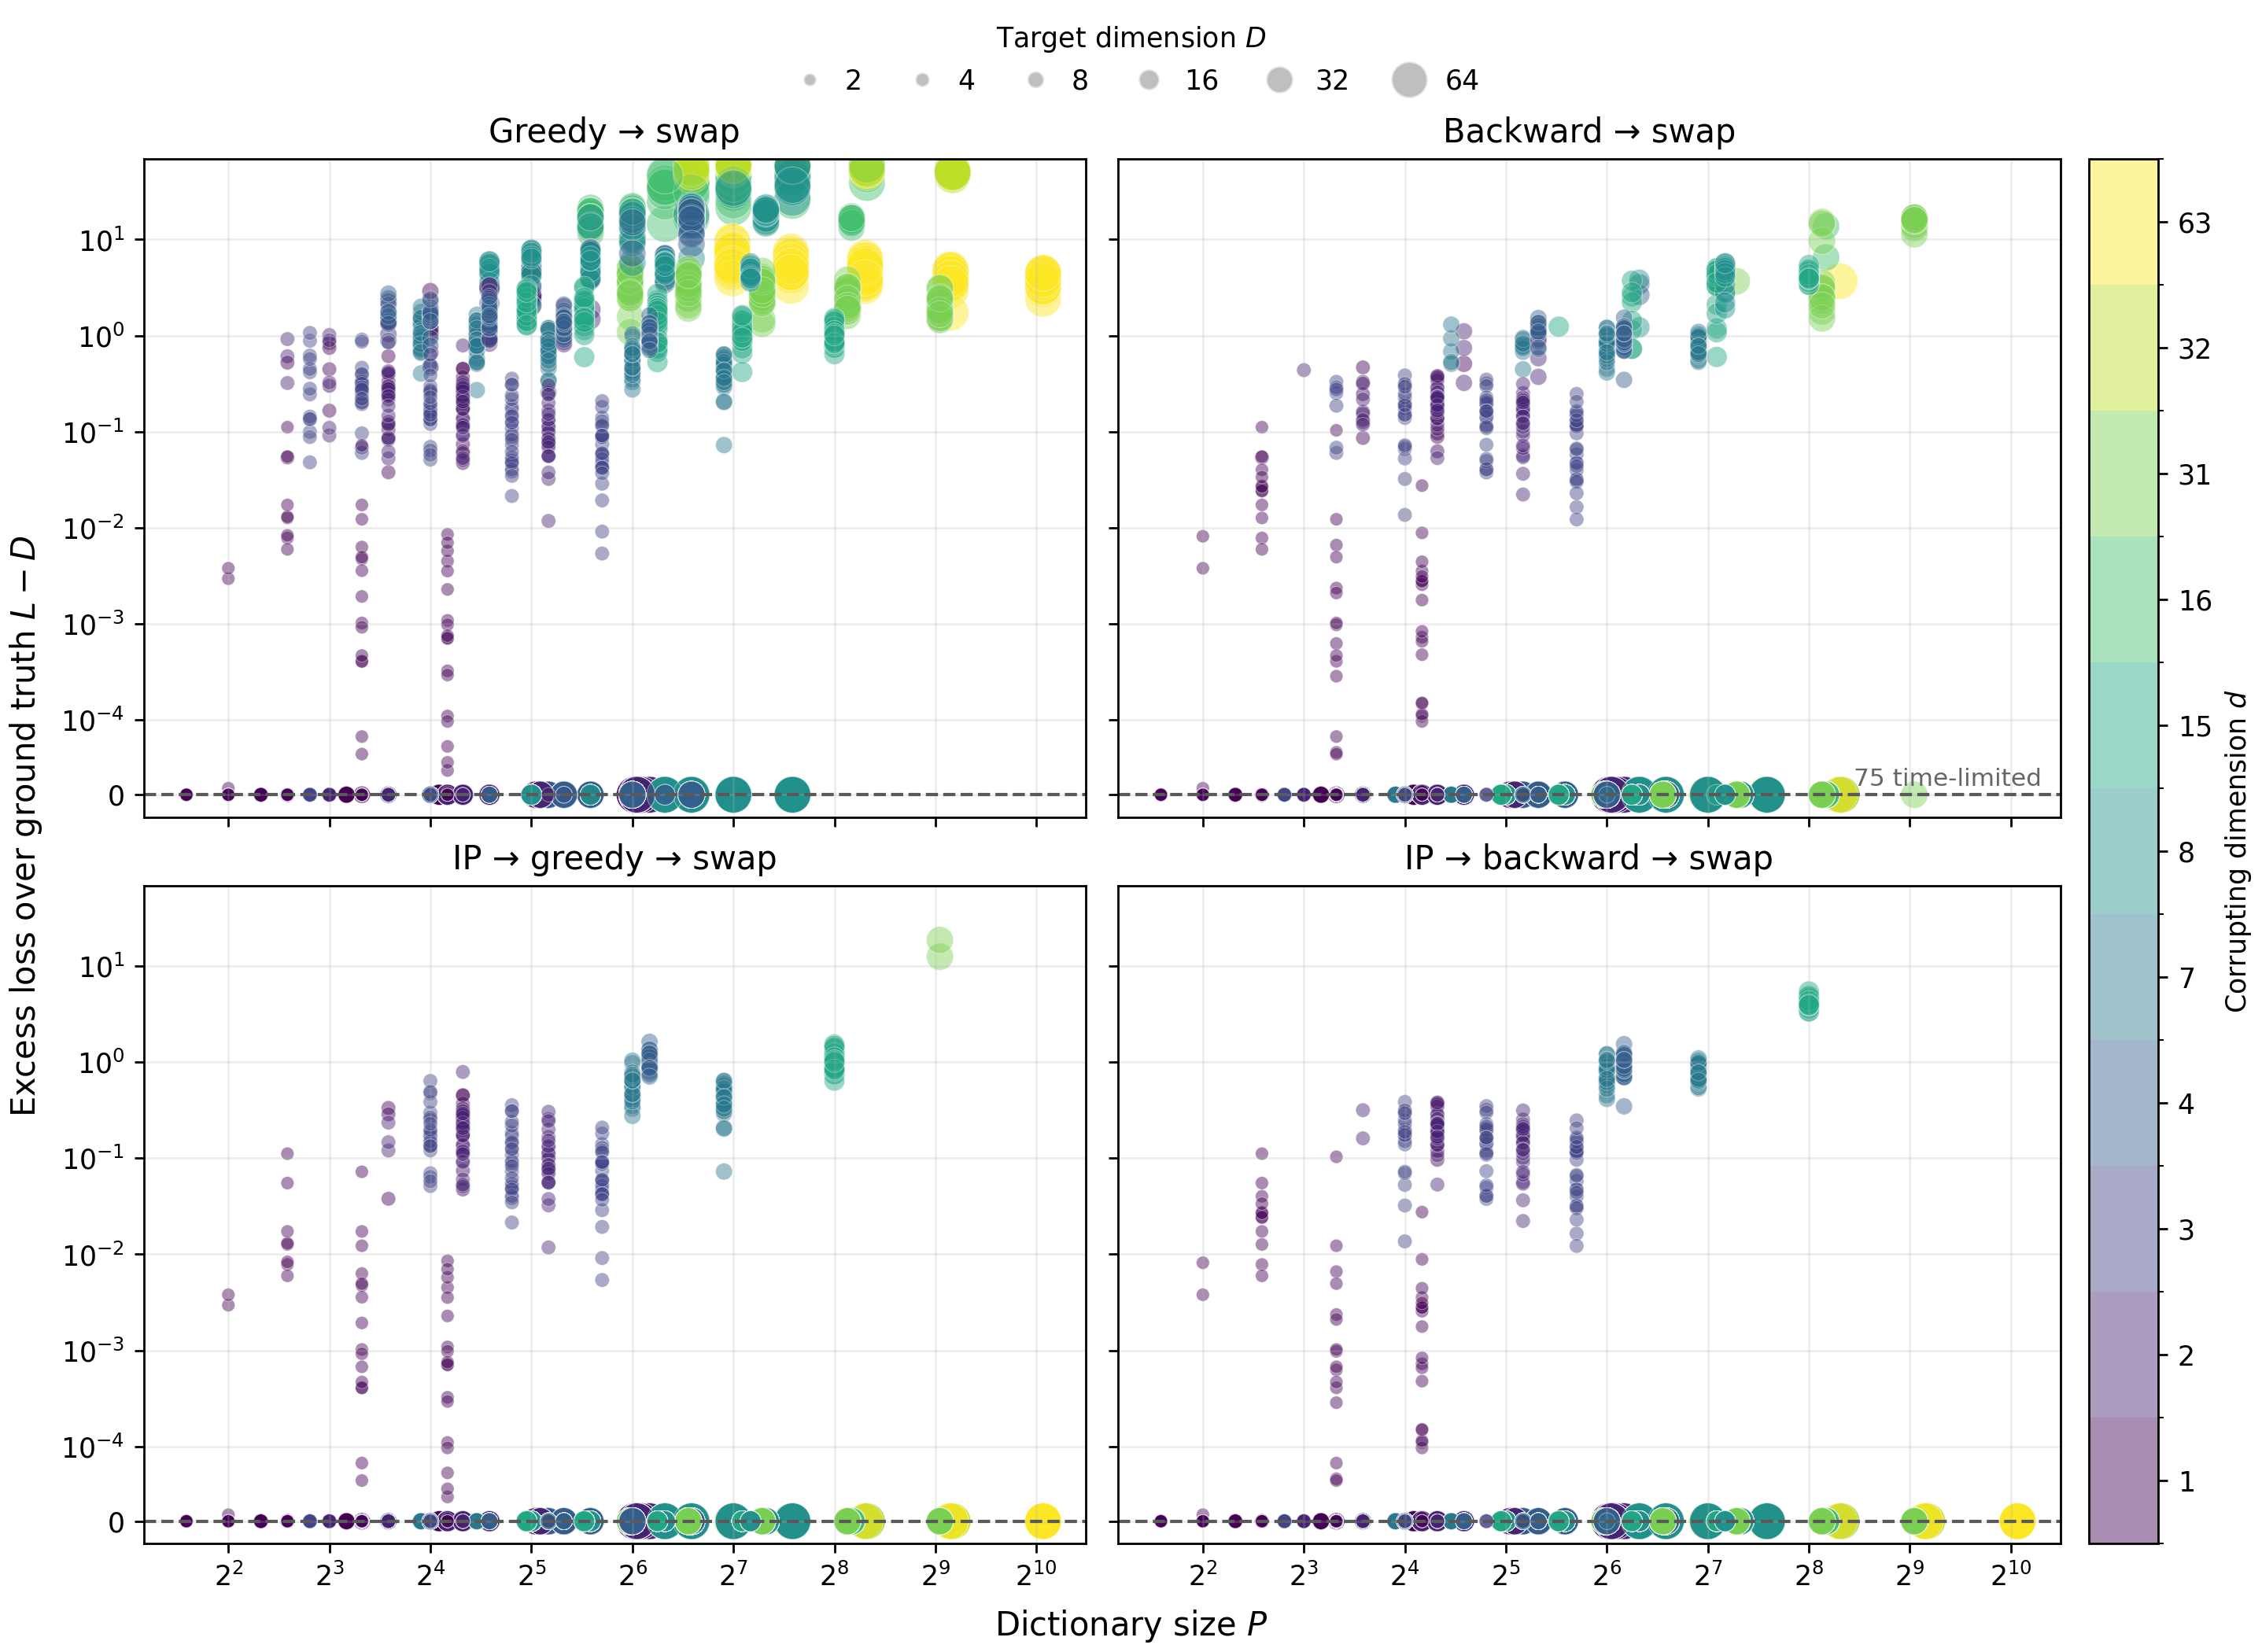
\includegraphics[width=\linewidth]{../figures/synthetic_excess_loss_vs_dictionary.png}
        \caption{Synthetic ground-truth regret.}
        \label{fig:synthetic-ground-truth-regret}
    \end{subfigure}\hfill
    \begin{subfigure}[t]{0.49\textwidth}
        \centering
        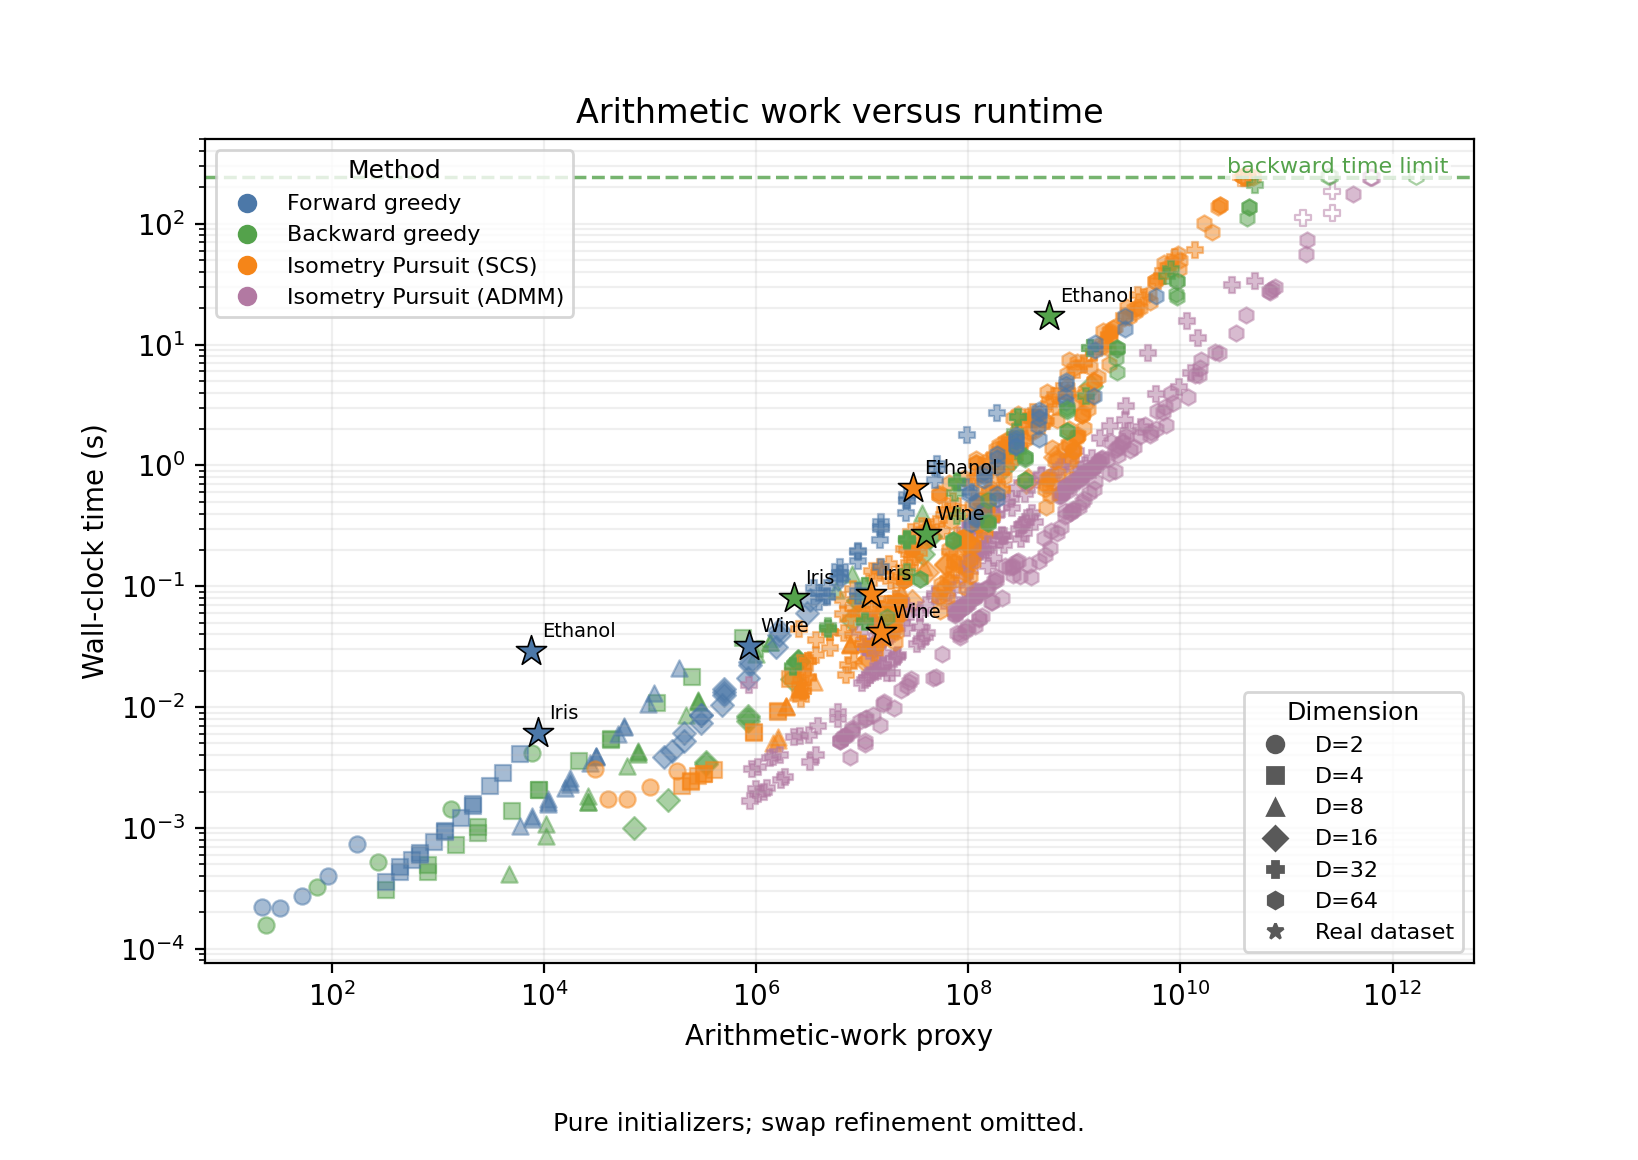
\includegraphics[width=\linewidth]{../figures/complexity_runtime/complexity_vs_runtime_overlay_with_early_stopping.png}
        \caption{Arithmetic work versus runtime.}
        \label{fig:complexity-runtime-early-stop}
    \end{subfigure}
    \caption{Statistical and computational behavior of the four search
    pipelines. (a) Ground-truth regret versus dictionary size in the synthetic
    identity-block experiments. The planted identity block attains raw loss
    $D$, so the vertical axis is $L-D$ and zero denotes optimal loss. Panels
    give the four search methods, point area encodes target dimension $D$, and
    color encodes corrupting dimension $d_c$. Each point is one replicate;
    text within the backward panels reports runs omitted by the arithmetic-work
    budget. (b) Arithmetic-work proxies versus measured wall-clock time for
    the pure forward, \isometrypursuit, and backward initializers; the common
    swap refinement is omitted. Synthetic points use task-aware stopping for
    \isometrypursuit, marker shape gives $D$, and stars denote real data. The
    green dashed line at $10^9$ is the backward-only work budget for the
    expanded synthetic sweep, not a wall-clock cutoff.}
\end{figure}

Our main interpretability dataset is the Ethanol dataset from \citet{Chmiela2018-at, Koelle2022-ju}.
For this dataset we evaluate a dictionary of interpretable features  - bond torsions - for their ability to parameterize the molecular configuration space.
In this interpretability use case, columns denote gradients of informative features.
We compute Jacobian matrices of putative parametrization functions and project them onto estimated tangent spaces (see \citet{Koelle2022-ju} for preprocessing details).
Rather than selecting between data points, we are selecting between functions which parameterize the data.
Replicates are created by sampling from data points and their corresponding tangent spaces are estimated in $B = 252$.
This dataset exemplifies our motivating example - the search for locally isometric embeddings.

\newcommand{\experimenttablerows}{%
Iris & 4 & 75 & 25 & 9.1 $\pm$ 1.2 & 6.7 $\pm$ 1 & 8 $\pm$ 1 & 0.8 & 0.04 & 1.9e-04 \\
Wine & 13 & 89 & 25 & 96 $\pm$ 9.3 & 26 $\pm$ 2.1 & 96 $\pm$ 8.9 & 0.12 & 0.56 & 0.36 \\
Ethanol & 2 & 756 & 25 & 2.8 $\pm$ 0.99 & 2.8 $\pm$ 0.4 & 2.8 $\pm$ 0.98 & 0.2 & 0.56 & 0.82 \\
}


\begin{table}[t]
\tiny
\centering
\resizebox{\textwidth}{!}{%
\begin{tabular}{|c|c|c|c|c|c|c|c|c|c|}
\toprule
Name & $D$ & $P$ & $R$ & $\ell(X_{.\widehat{S}_{FB}})$ & $|\widehat{S}_{IP}|$ & $\ell(X_{.\widehat{S}_{FB \mid IP}})$ &
\begin{tabular}{c}
$\widehat P (\ell(X_{.\widehat{S}_{FB}}) >$ \\
$\ell(X_{.\widehat{S}_{FB \mid IP}}))$
\end{tabular} &
\begin{tabular}{c}
$\widehat P (\ell(X_{.\widehat{S}_{FB}}) =$ \\
$\ell(X_{.\widehat{S}_{FB \mid IP}}))$
\end{tabular} &
\begin{tabular}{c}
Paired $t$-test \\
$p$-value
\end{tabular} \\
\midrule
\experimenttablerows
\bottomrule
\end{tabular}
}
\caption{Experimental parameters and results.
For Iris and Wine, probability estimates $\widehat P$ result from random downsampling features $[P]$ by a factor of $2$ to create $R$ replicates, while for Ethanol, replicates correspond to individual data points.
Distributional probabilities $\widehat P (\ell(X_{.\widehat{S}_{FB}}) > \ell(X_{.\widehat{S}_{FB \mid IP}}))$ and $\widehat P (\ell(X_{.\widehat{S}_{FB}}) = \ell(X_{.\widehat{S}_{FB \mid IP}}))$ are empirical across replicates.
Here $\widehat{S}_{FB}$ denotes the support selected by full-dictionary forward-backward search, and $\widehat{S}_{FB \mid IP}$ denotes the support selected by forward-backward search after restricting the dictionary to $\widehat{S}_{IP}$.
The final column reports the one-sided paired $t$-test $p$-value for the alternative that full-dictionary forward-backward losses exceed restricted forward-backward losses.
}
\label{tab:experiments}
\end{table}

To compare all four practical searches directly, define the replicate-level
oracle loss as $\ell_r^\star=\min_m \ell_{m,r}$ and the oracle regret of method
$m$ as $\mathcal R_{m,r}=\ell_{m,r}-\ell_r^\star$.
Table~\ref{tab:oracle-regret} reports both the empirical probability of attaining
the oracle loss and the mean oracle regret.

Figure \ref{fig:synthetic-support-recovery} reports exact recovery rates in the synthetic identity-block experiments.
Figure \ref{fig:synthetic-ground-truth-regret} compares losses against the known
ground-truth optimum, while Figure \ref{fig:synthetic-support-size} shows how
aggressively \isometrypursuit~screens the candidate dictionary.
Table \ref{tab:experiments} compares the final isometry losses from full-dictionary forward-backward search with losses from forward-backward search inside the \isometrypursuit~ support.
Table \ref{tab:experiments} and Figure \ref{fig:support_cardinalities} detail intermediate support recovery cardinalities from \isometrypursuit.
Isometry pursuit substantially reduced the size of the dictionary and made second-stage search computationally feasible.
Figure \ref{fig:complexity-runtime-early-stop} shows that the arithmetic-work
proxies track observed runtime and that task-aware stopping substantially reduces
the \isometrypursuit~cost.  The $10^9$ backward-search boundary is a conservative
aggregate budget for the replicated sweep: individual problems just beyond it
may still be inexpensive, whereas the largest omitted settings exceed it by
more than an order of magnitude. Additional wall-clock summaries are given in
Section \ref{sec:timing}.

\section{Discussion}
\label{sec:discussion}

We have shown that column normalization and multitask basis pursuit can help select isometric submatrices from wide dictionaries, both by improving selections and by reducing the cost of subsequent search.
The normalization favors unit-length candidates, while multitask basis pursuit favors orthogonality.
Many full-rank $D$-column submatrices can represent $I_D$, so our objective distinguishes geometric quality among representations of the same cardinality, extending the usual sparse-recovery perspective of greedy and convex basis pursuit \citep{Mallat93-wi, Tropp05-ml, Chen2001-hh, Tropp06-sg}.
Compared with Sparse PCA \citep{DAspremont2007-aq, Dey2017-mx, Bertsimas2022-qo, Bertsimas2022-dv}, we select existing columns rather than linear combinations of them.
A multitask Lasso extension could vary sparsity along a regularization path, while selecting fewer than $D$ columns and using response matrices other than $I_D$ would extend the coordinate-selection problem \citep{Hastie2015-qa, Mishkin2022-yf}.
Sampling incoming columns could reduce swap costs, while beam search could retain several candidate subsets at each step to explore competing selection paths on either the full or screened dictionary \citep{Zou2024-swap, Fraiman2022-beam}.

Our experiments illustrate two applications of the same column-selection problem: diversification selects observations, while interpretable coordinate estimation selects functions through their tangent-space gradients.
Recommendation and retrieval, including document selection for language-model question answering \citep{Chen2024-esrag}, provide further settings for selecting observations or embedding vectors.
\citet{Okajima2026-nnn} select documents by reconstructing the query embedding as a sparse nonnegative combination of document embeddings, giving a direct example of convex selection for retrieval.
With unit-norm embeddings, the first nonzero coefficients on this nonnegative elastic-net regularization path select documents with maximum positive cosine similarity to the query.
% KKT at zero gives X_{.p}^T y <= lambda_1; positive maximizers enter first as lambda_1 decreases, with lambda_2 fixed.
ColBERT, for example, represents queries and documents with token embeddings and sums the maximum similarity of each query embedding to a document embedding \citep{Khattab2020-colbert}.
This supplies a concrete setting in which to investigate whether selecting less redundant embedding vectors can preserve retrieval quality while reducing the number of vectors compared.
Greedy diversification methods already seek to reduce redundancy in retrieved results \citep{Carbonell1998-ji}; our results motivate testing convex screening alongside such searches, with the geometric criterion and selected dictionary adapted to the application.
% TODO (Sam): Add a citation supporting diversification applications in recommendation.


\newpage

\bibliography{ref}

\newpage

%\section*{NeurIPS Paper Checklist}


\begin{enumerate}

\item {\bf Claims}
    \item[] Question: Do the main claims made in the abstract and introduction accurately reflect the paper's contributions and scope?
    \item[] Answer: \answerYes% Replace by \answerYes{}, \answerNo{}, or \answerNA{}.
    \item[] Justification: Yes they do


\item {\bf Limitations}
    \item[] Question: Does the paper discuss the limitations of the work performed by the authors?
    \item[] Answer: \answerYes{} % Replace by \answerYes{}, \answerNo{}, or \answerNA{}.
    \item[] Justification: We discuss that we can't necessarily find the optimum, just in the special case where a certain type of optimum is present{}


\item {\bf Theory assumptions and proofs}
    \item[] Question: For each theoretical result, does the paper provide the full set of assumptions and a complete (and correct) proof?
    \item[] Answer: \answerYes % Replace by \answerYes{}, \answerNo{}, or \answerNA{}.
    \item[] Justification: We do provide intuition in the main text and reference relevant background.  Proofs are in supplement.


    \item {\bf Experimental result reproducibility}
    \item[] Question: Does the paper fully disclose all the information needed to reproduce the main experimental results of the paper to the extent that it affects the main claims and/or conclusions of the paper (regardless of whether the code and data are provided or not)?
    \item[] Answer: \answerYes{} % Replace by \answerYes{}, \answerNo{}, or \answerNA{}.
    \item[] Justification: All experimental processing code is released and execution is sketched out in a satisfactory level of detail


\item {\bf Open access to data and code}
    \item[] Question: Does the paper provide open access to the data and code, with sufficient instructions to faithfully reproduce the main experimental results, as described in supplemental material?
    \item[] Answer: \answerYes{} % Replace by \answerYes{}, \answerNo{}, or \answerNA{}.
    \item[] Justification: These are in the linked GitHub repository and discussed in the paper.{}



\item {\bf Experimental setting/details}
    \item[] Question: Does the paper specify all the training and test details (e.g., data splits, hyperparameters, how they were chosen, type of optimizer, etc.) necessary to understand the results?
    \item[] Answer: \answerYes{} % Replace by \answerYes{}, \answerNo{}, or \answerNA{}.
    \item[] Justification: In addition to the above code we provide a table detailing experimental parameters{}
    \item[] Guidelines:

\item {\bf Experiment statistical significance}
    \item[] Question: Does the paper report error bars suitably and correctly defined or other appropriate information about the statistical significance of the experiments?
    \item[] Answer: \answerYes{} % Replace by \answerYes{}, \answerNo{}, or \answerNA{}.
    \item[] Justification: We provide error bars for statistics like support cardinality when appropriate

\item {\bf Experiments compute resources}
    \item[] Question: For each experiment, does the paper provide sufficient information on the computer resources (type of compute workers, memory, time of execution) needed to reproduce the experiments?
    \item[] Answer: \answerYes{} % Replace by \answerYes{}, \answerNo{}, or \answerNA{}.
    \item[] Justification: We provide timing and computational details for the experiments run in the paper{}

\item {\bf Code of ethics}
    \item[] Question: Does the research conducted in the paper conform, in every respect, with the NeurIPS Code of Ethics \url{https://neurips.cc/public/EthicsGuidelines}?
    \item[] Answer: \answerYes{} % Replace by \answerYes{}, \answerNo{}, or \answerNA{}.
    \item[] Justification: This paper has no societal harms - if anything the research program this is a part of (interpretability) should cause some benefits.  

\item {\bf Broader impacts}
    \item[] Question: Does the paper discuss both potential positive societal impacts and negative societal impacts of the work performed?
    \item[] Answer: \answerNA{} % Replace by \answerYes{}, \answerNo{}, or \answerNA{}.
    \item[] Because this paper is fairly theoretical, we do not discuss broader impacts.

    
\item {\bf Safeguards}
    \item[] Question: Does the paper describe safeguards that have been put in place for responsible release of data or models that have a high risk for misuse (e.g., pretrained language models, image generators, or scraped datasets)?
    \item[] Answer: \answerNA {} % Replace by \answerYes{}, \answerNo{}, or \answerNA{}.
    \item[] Justification: No such risks


\item {\bf Licenses for existing assets}
    \item[] Question: Are the creators or original owners of assets (e.g., code, data, models), used in the paper, properly credited and are the license and terms of use explicitly mentioned and properly respected?
    \item[] Answer: \answerYes{} % Replace by \answerYes{}, \answerNo{}, or \answerNA{}.
    \item[] Justification: We have cited the data sources used in the paper 


\item {\bf New assets}
    \item[] Question: Are new assets introduced in the paper well documented and is the documentation provided alongside the assets?
    \item[] Answer: \answerNA {} % Replace by \answerYes{}, \answerNo{}, or \answerNA{}.
    \item[] Justification: No new assets


\item {\bf Crowdsourcing and research with human subjects}
    \item[] Question: For crowdsourcing experiments and research with human subjects, does the paper include the full text of instructions given to participants and screenshots, if applicable, as well as details about compensation (if any)? 
    \item[] Answer: \answerNA {} % Replace by \answerYes{}, \answerNo{}, or \answerNA{}.
    \item[] Justification: Not used
    \item[] Guidelines:



\item {\bf Institutional review board (IRB) approvals or equivalent for research with human subjects}
    \item[] Question: Does the paper describe potential risks incurred by study participants, whether such risks were disclosed to the subjects, and whether Institutional Review Board (IRB) approvals (or an equivalent approval/review based on the requirements of your country or institution) were obtained?
    \item[] Answer: \answerNA {} % Replace by \answerYes{}, \answerNo{}, or \answerNA{}.
    \item[] Justification: Not relevant{}


\item {\bf Declaration of LLM usage}
    \item[] Question: Does the paper describe the usage of LLMs if it is an important, original, or non-standard component of the core methods in this research? Note that if the LLM is used only for writing, editing, or formatting purposes and does not impact the core methodology, scientific rigorousness, or originality of the research, declaration is not required.
    %this research? 
    \item[] Answer: \answerNA{} % Replace by \answerYes{}, \answerNo{}, or \answerNA{}.
    \item[] Justification: No non-standard LLM usage

\end{enumerate}

\newpage

\section{Supplement}

This section contains algorithms, proofs, and experiments in support of the main text.

\subsection{Algorithms}
\label{sec:algorithms}

Greedy algorithms are computationally expedient but can get stuck in local optima \citep{Cormen, Russell-09}, even with randomized restarts \citep{Dick2014HowMR}.

\begin{algorithm}[H]
\caption{\greedy(Matrix ${X} \in \mathbb{R}^{D \times P}$, objective $f$)}
\begin{algorithmic}[1]
\STATE {\bf Initialize} $S = \emptyset$
\WHILE{$|S| < D$}
    \STATE {\bf Initialize} $S_{\text{best}} = S$
    \STATE {\bf Initialize} $f_{\text{best}} = \infty$
    \FOR{each $p \in \{1, 2, \dots, P\} \setminus S$}
        \STATE {\bf Evaluate} $f({X}_{.(S \cup \{p\})})$
        \IF{$f({X}_{.(S \cup \{p\})}) < f_{\text{best}}$}
            \STATE {\bf Update} $S_{\text{best}} = S \cup \{p\}$
            \STATE {\bf Update} $f_{\text{best}} = f(\mathcal{X}_{.(S \cup \{p\})})$
        \ENDIF
    \ENDFOR
    \STATE {\bf Update} $S = S_{\text{best}}$
\ENDWHILE
\STATE {\bf Return} $S$
\end{algorithmic}
\end{algorithm}

\begin{algorithm}[H]
\caption{\backwardgreedy(Matrix ${X} \in \mathbb{R}^{D \times P}$, objective $f$)}
\begin{algorithmic}[1]
\STATE {\bf Initialize} $S = \{1, 2, \dots, P\}$
\WHILE{$|S| > D$}
    \STATE {\bf Initialize} $S_{\text{best}} = S$
    \STATE {\bf Initialize} $f_{\text{best}} = \infty$
    \FOR{each $p \in S$}
        \STATE {\bf Evaluate} $f({X}_{.(S \setminus \{p\})})$
        \IF{$f({X}_{.(S \setminus \{p\})}) < f_{\text{best}}$}
            \STATE {\bf Update} $S_{\text{best}} = S \setminus \{p\}$
            \STATE {\bf Update} $f_{\text{best}} = f(\mathcal{X}_{.(S \setminus \{p\})})$
        \ENDIF
    \ENDFOR
    \STATE {\bf Update} $S = S_{\text{best}}$
\ENDWHILE
\STATE {\bf Return} $S$
\end{algorithmic}
\end{algorithm}

Our swap search evaluates every selected--unselected column pair and takes the best improving swap, as in local search for cardinality-constrained D-optimal design \citep{Fedorov1972-optimal,Wang2025-doptimal} and column selection \citep{Gu1996-strong-rrqr}.
Zou et al.\ instead sample an incoming column and evaluate its possible swaps for reconstruction-based column selection \citep{Zou2024-swap}.
We initialize with forward selection or backward elimination \citep{Mao2004-forward-backward}; related FoBa methods alternate additions and deletions rather than jointly choosing a swap \citep{Zhang2008-foba,pmlr-v32-liub14}.

\begin{algorithm}[H]
\caption{\forwardbackward(Matrix ${X} \in \mathbb{R}^{D \times P}$, objective $f$)}
\begin{algorithmic}[1]
\STATE {\bf Initialize} $S \leftarrow$ \greedy(${X}$, $f$)
\STATE {\bf Initialize} $f_{\text{current}} \leftarrow f({X}_{.S})$
\FOR{$p = 1, 2, \dots, P$}
    \STATE {\bf Initialize} $S_{\text{best}} \leftarrow S$
    \STATE {\bf Initialize} $f_{\text{best}} \leftarrow f_{\text{current}}$
    \FOR{each $j \in \{1, 2, \dots, P\} \setminus S$}
        \FOR{each $q \in S$}
            \STATE {\bf Initialize} $S_{\text{candidate}} = (S \cup \{j\}) \setminus \{q\}$
            \STATE {\bf Evaluate} $f({X}_{.S_{\text{candidate}}})$
            \IF{$f({X}_{.S_{\text{candidate}}}) < f_{\text{best}}$}
                \STATE {\bf Update} $S_{\text{best}} \leftarrow S_{\text{candidate}}$
                \STATE {\bf Update} $f_{\text{best}} \leftarrow f({X}_{.S_{\text{candidate}}})$
            \ENDIF
        \ENDFOR
    \ENDFOR
    \IF{$S_{\text{best}} = S$}
        \STATE {\bf Break}
    \ENDIF
    \STATE {\bf Update} $S \leftarrow S_{\text{best}}$
    \STATE {\bf Update} $f_{\text{current}} \leftarrow f_{\text{best}}$
\ENDFOR
\STATE {\bf Return} $S$
\end{algorithmic}
\end{algorithm}

\subsection{Proofs}
\label{sec:proofs}

\subsubsection{Proofs in support of Table~\ref{tab:losses}}
\label{sec:table1_proofs}

\paragraph{Chen--Meil\u{a}.}
\label{sec:chen_meila_loss}
Chen--Meil\u{a} denote the manifold dimension by $d$ and the number of candidate functions by $m$; these are our $D$ and $P$.
We retain $S$ for the selected index set and drop the observation index and averaging to compare losses at a single point.
They write $U(i)\in\mathbb R^{m\times d}$ for an orthonormal basis of the embedded tangent space at observation $i$, $U_S(i)$ for its rows indexed by $S$, and $u_k^S(i)$ for column $k$ of $U_S(i)$.
In our notation, $X=U(i)^T\in\mathbb R^{D\times P}$, so $U_S(i)=X_{.S}^T$ and $\|u_d^S(i)\|_2=\|X_{dS}\|_2$.
Their candidate functions are Laplacian eigenfunctions; we denote them by $f_p$ and their eigenvalues by $\lambda_p$.
For $|S|\geq D$ and $1\in S$, their objective averages the following quantity over observations \citep[Eq.~(2)]{NEURIPS2019_6a10bbd4}:
\begin{align}
\mathcal L_i(S;\zeta)
&=\frac12\log\det(U_S(i)^TU_S(i))-\sum_{d=1}^D\log\|u_d^S(i)\|_2-\zeta\sum_{p\in S}\lambda_p.
\end{align}
Setting $\zeta=0$ and negating their objective gives the loss in Table~\ref{tab:losses}:
\begin{align}
-\mathcal L_i(S;0)
&=-\frac12\log\det(X_{.S}X_{.S}^T)+\sum_{d=1}^D\log\|X_{dS}\|_2\\
&=-\log\frac{\det(X_{.S}X_{.S}^T)^{1/2}}{\prod_{d=1}^D\|X_{dS}\|_2}.
\end{align}

\paragraph{Kohli et al.}
\label{proof:distortion_is_condition_number}
\citet[Eqs.~(1)--(3)]{Kohli2021-lr} define neighborhood distortion as the product of the largest distance expansion and the largest distance contraction:
\begin{align}
\operatorname{Distortion}(f_{.S},B)
&=\left(\sup_{\xi'\ne\xi''\in B}\frac{\|f_{.S}(\xi')-f_{.S}(\xi'')\|_2}{d_{\mathcal M}(\xi',\xi'')}\right)
\left(\sup_{\xi'\ne\xi''\in B}\frac{d_{\mathcal M}(\xi',\xi'')}{\|f_{.S}(\xi')-f_{.S}(\xi'')\|_2}\right)\\
&=\frac{\sup_{\xi'\ne\xi''\in B}r_S(\xi',\xi'')}{\inf_{\xi'\ne\xi''\in B}r_S(\xi',\xi'')},
\qquad r_S(\xi',\xi'')=\frac{\|f_{.S}(\xi')-f_{.S}(\xi'')\|_2}{d_{\mathcal M}(\xi',\xi'')},
\end{align}
where $d_{\mathcal M}$ is geodesic distance.

\begin{proposition}
\label{prop:distortion_is_condition_number}
If $f_{.S}$ is continuously differentiable near $\xi$ and $Df_{.S}(\xi)$ is invertible, then, with $\operatorname{Distortion}$ defined above and $B_{\mathcal M}(\xi,\varepsilon)$ denoting the geodesic ball of radius $\varepsilon$ centered at $\xi$,
\begin{align}
\lim_{\varepsilon\to 0}
\operatorname{Distortion}\!\left(f_{.S},B_{\mathcal M}(\xi,\varepsilon)\right)
=\frac{\sigma_1\!\left(Df_{.S}(\xi)\right)}
       {\sigma_D\!\left(Df_{.S}(\xi)\right)},
\end{align}
the condition number of $Df_{.S}(\xi)$ \citep{GolubWilkinson-condition,Boyd2004-ql}.
\end{proposition}

\begin{proof}
For distinct $\xi',\xi''\in B_{\mathcal M}(\xi,\varepsilon)$, let $u',u''$ be their local coordinates, chosen so that the coordinate tangent basis at $\xi$ is orthonormal.
Smoothness of $\mathcal M$ gives $d_{\mathcal M}(\xi',\xi'')=\|u'-u''\|_2(1+o(1))$, while continuous differentiability of $f_{.S}$ gives $f_{.S}(\xi')-f_{.S}(\xi'')=Df_{.S}(\xi)(u'-u'')+o(\|u'-u''\|_2)$, uniformly over pairs as $\varepsilon\to0$.
Dividing by their separation therefore gives
\begin{align}
r_S(\xi',\xi'')
=\frac{\|Df_{.S}(\xi)(u'-u'')\|_2}{\|u'-u''\|_2}+o(1).
\end{align}
Thus $\sup r_S\to\sigma_1(Df_{.S}(\xi))$ and $\inf r_S\to\sigma_D(Df_{.S}(\xi))$.
When the differential is invertible, taking their quotient gives $\operatorname{Distortion}(f_{.S},B_{\mathcal M}(\xi,\varepsilon)) \to\sigma_1(Df_{.S}(\xi))/\sigma_D(Df_{.S}(\xi))$.
\end{proof}

\begin{proposition}
The condition number is minimized by conformal maps.
\end{proposition}


\subsubsection{Proof of Proposition \ref{prop:sdiv_singular_values}}
\label{proof:sdiv_singular_values}

\begin{restatedproposition}{prop:sdiv_singular_values}
If $X^T X$ is positive definite, then $D(X^T X,I_D)^2 = \sum_{d=1}^D \log \frac{\sigma_d(X) + \sigma_d(X)^{-1}}{2}$.
\end{restatedproposition}

\begin{proof}
First,
\begin{align}
\frac{1}{2}\log \det(X^T X) &= \frac{1}{2} \log \prod_{d=1}^D \sigma_d(X)^2 \\
&= \log \prod_{d=1}^D \sigma_d(X) \\
&= \sum_{d=1}^D \log \sigma_d(X).
\end{align}
Secondly, $I_D$ and $X^T X$ are diagonalizable in the same basis, so
\begin{align}
\log \det (\frac{X^T X + I_D}{2}) &= \log \prod_{d=1}^D \frac{\sigma_d(X)^2 + 1}{2} \\
&= \sum_{d=1}^D \log \frac{\sigma_d(X)^2 + 1}{2}.
\end{align}
Then,
\begin{align}
D(X^T X,I_D)^2
&= \sum_{d=1}^D (\log \frac{\sigma_d(X)^2 + 1}{2} - \log \sigma_d(X)) \\
&= \sum_{d=1}^D \log \frac{\sigma_d(X)^2 + 1}{2 \sigma_d(X)} \\
&= \sum_{d=1}^D \log \frac{\sigma_d(X) + \sigma_d(X)^{-1}}{2}.
\end{align}
\end{proof}

\subsubsection{Proof of Proposition \ref{prop:normalized_spectral_losses}}
\label{proof:normalized_spectral_losses}

\begin{restatedproposition}{prop:normalized_spectral_losses}
For full-rank $X\in\mathbb R^{D\times D}$, let $g:(0,\infty)\to\mathbb R$ be twice differentiable with $g(1)=0$, $g'(t)<0$, and $t g''(t)>g'(t)$ for every $t>0$.
Use $q$ from~\eqref{eq:normalization}.
Then $\ell_{g,q}(X)=\sum_{d=1}^D g\!\left(\sigma_d(n_q^{\times D}(X))\right)$ is nonnegative and satisfies Properties~\ref{property:rotation_invariance}--\ref{property:pathwise}.
\end{restatedproposition}

\begin{proof}
\paragraph{Property~\ref{property:rotation_invariance} (Rotation invariance).}
\emph{``A matrix loss $\ell$ is rotation invariant if, for every orthonormal $U\in\mathbb R^{D\times D}$, $\ell(UX)=\ell(X)$.''}

We first check that column normalization commutes with orthonormal transformations.
For orthonormal $U$, column normalization gives $n_q^{\times D}(UX)=U n_q^{\times D}(X)$.
Since $U n_q^{\times D}(X)$ and $n_q^{\times D}(X)$ have the same singular values, $\ell_{g,q}(UX)=\ell_{g,q}(X)$, which proves Property~\ref{property:rotation_invariance}.

\paragraph{Property~\ref{property:unique_isometry_minimum} (Unique isometry minimum).}
\emph{``A matrix loss $\ell$ is uniquely minimized by isometries if $\arg\min_X\ell(X)=\{X:XX^T=I_D\}$.''}

\textbf{Nonnegativity: $\ell_{g,q}(X)\geq0$.}
We first bound the average squared singular value of $n_q^{\times D}(X)$ by one.
Write $u_d=\sigma_d(n_q^{\times D}(X))^2$.
The squared singular values of a matrix are the eigenvalues of its Gram matrix, so their sum equals its trace and hence its squared Frobenius norm.
Since the $d$th column of $n_q^{\times D}(X)$ has norm $q(\|x_{.d}\|_2)$ and $q(t)\leq1$ with equality only at $t=1$,
\begin{align}
\frac{1}{D}\sum_{d=1}^D u_d
&=\frac{\|n_q^{\times D}(X)\|_F^2}{D} \\
&=\frac{1}{D}\sum_{d=1}^D q(\|x_{.d}\|_2)^2 \\
&\leq1.
\end{align}

We next show that $\widetilde g(u)=g(\sqrt u)$ is strictly convex and decreasing on $(0,\infty)$.
Then $\widetilde g(1)=0$, and
\begin{align}
\widetilde g'(u)&=\frac{g'(\sqrt u)}{2\sqrt u} \\
&<0, \\
\widetilde g''(u)&=\frac{\sqrt u\,g''(\sqrt u)-g'(\sqrt u)}{4u^{3/2}} \\
&>0.
\end{align}

We now use this bound to show that the loss is nonnegative.
The loss evaluates these squared singular values through $\widetilde g$, since $\ell_{g,q}(X)=\sum_{d=1}^D\widetilde g(u_d)$.
Jensen's inequality for the strictly convex function $\widetilde g$, followed by its monotonic decrease, gives
\begin{align}
\frac{1}{D}\sum_{d=1}^D \widetilde g(u_d)
&\geq \widetilde g\!\left(\frac{1}{D}\sum_{d=1}^D u_d\right) \label{eq:normalized_spectral_jensen} \\
&\geq \widetilde g(1) \label{eq:normalized_spectral_decreasing_bound} \\
&=0.
\end{align}
Hence $\ell_{g,q}(X)\geq0$.

\textbf{Zero loss implies $X^\top X=I_D$.}
We determine when equality holds in the nonnegativity bound.
Equality in Jensen's inequality~\eqref{eq:normalized_spectral_jensen}, by strict convexity, requires $u_1=\cdots=u_D$, while equality in~\eqref{eq:normalized_spectral_decreasing_bound} requires $D^{-1}\sum_d u_d=1$.
Thus every singular value of $n_q^{\times D}(X)$ equals one.
Zero loss forces equality throughout the nonnegativity bound, so the identity between squared singular values and squared column norms gives $\sum_{d=1}^D q(\|x_{.d}\|_2)^2=D$.
Moreover, equality in $\sum_{d=1}^D q(\|x_{.d}\|_2)^2\leq D$ requires $\|x_{.d}\|_2=1$ for every $d$.
Consequently $n_q^{\times D}(X)=X$ and $X^\top X=I_D$.

\textbf{$X^\top X=I_D$ implies zero loss.}
Conversely, if $X^\top X=I_D$, every column has unit norm, so $n_q^{\times D}(X)=X$.
Every singular value then equals one, and $g(1)=0$ gives $\ell_{g,q}(X)=0$.
Thus the loss is nonnegative and equals zero if and only if $X^\top X=I_D$, proving Property~\ref{property:unique_isometry_minimum}.


\paragraph{Property~\ref{property:log_symmetry} (Column log symmetry).}
\emph{``A matrix loss $\ell$ is column log-symmetric if replacing any nonzero column $x_{.p}$ by $x_{.p}/\|x_{.p}\|_2^2$, with all other columns fixed, leaves $\ell$ unchanged.''}

We check that reciprocating a column length leaves its normalized value unchanged.
$q(t)=q(t^{-1})$ gives $n_q(v)=n_q(v/\|v\|_2^2)$.
Reciprocating any column's length therefore leaves $n_q^{\times D}(X)$ unchanged, which proves Property~\ref{property:log_symmetry}.


\paragraph{Property~\ref{property:pathwise} (Column-rescaling monotonicity).}
\emph{``A matrix loss $\ell$ is column-rescaling monotone if, for every column $x_{.d}$, $\frac{\partial\ell}{\partial\|x_{.d}\|_2}$ is negative, zero, or positive when $\|x_{.d}\|_2<1$, $\|x_{.d}\|_2=1$, or $\|x_{.d}\|_2>1$, respectively.''}

We determine the sign of the loss derivative as one column length varies.
Fix all column directions and all columns except the $p$th, and write $r=\|x_{.p}\|_2$.
For a unit vector $v$ in its direction,
\begin{align}
n_q^{\times D}(X)n_q^{\times D}(X)^\top=A+q(r)^2vv^\top
\end{align}
for a fixed positive-semidefinite matrix $A$.
We compute the derivative using the eigenvalues $\lambda_d$ and orthonormal eigenvectors $z_d$ of $A+q(r)^2vv^\top$.
Spectral differentiation gives
\begin{align}
\frac{\partial\ell_{g,q}(X)}{\partial r}
=2q(r)q'(r)\sum_{d=1}^D\widetilde g'(\lambda_d)(z_d^\top v)^2.
\end{align}
Each $\widetilde g'(\lambda_d)$ is negative, and $\sum_{d=1}^D(z_d^\top v)^2=1$ because the eigenvectors form an orthonormal basis and $v$ has unit norm.
The sum is therefore strictly negative, so the derivative has the opposite sign to $q'(r)$.
Since $q$ is strictly increasing below one, stationary at one, and strictly decreasing above one, the derivative of $\ell_{g,q}$ with respect to $\|x_{.p}\|_2$ has exactly the signs in Property \ref{property:pathwise}.


\end{proof}

\subsubsection{Proofs of Propositions
\ref{prop:determinant_singular_values} and \ref{prop:frobenius_inverse_singular_values}}

\begin{restatedproposition}{prop:determinant_singular_values}
For full-rank $X\in\mathbb R^{D\times D}$, the centered inverse determinant $|\det(n_q^{\times D}(X))|^{-1}-1$ ranks candidate matrices in the same order as $\ell_{g,q}(X)$ with $g(t)=-\log t$.
\end{restatedproposition}

\begin{restatedproposition}{prop:frobenius_inverse_singular_values}
For full-rank $X\in\mathbb R^{D\times D}$, the centered inverse Frobenius norm $\|(n_q^{\times D}(X))^{-1}\|_F-\sqrt D$ ranks candidate matrices in the same order as $\ell_{g,q}(X)$ with $g(t)=t^{-2}-1$.
\end{restatedproposition}

\begin{proof}
The determinant is the product of the singular values, so
\begin{align}
|\det(n_q^{\times D}(X))|^{-1}-1
&=\prod_{d=1}^D\sigma_d(n_q^{\times D}(X))^{-1}-1 \\
&=\exp\left(-\sum_{d=1}^D\log\sigma_d(n_q^{\times D}(X))\right)-1 \\
&=\exp(\ell_{g,q}(X))-1
\end{align}
for $g(t)=-\log t$.
Since $t\mapsto\exp(t)-1$ is strictly increasing, comparing the centered inverse determinants gives exactly the same ranking as comparing $\ell_{g,q}$.

For the inverse Frobenius norm, the singular values of $(n_q^{\times D}(X))^{-1}$ are $\sigma_d(n_q^{\times D}(X))^{-1}$, and hence
\begin{align}
\|(n_q^{\times D}(X))^{-1}\|_F-\sqrt D
&=\left(\sum_{d=1}^D\sigma_d(n_q^{\times D}(X))^{-2}\right)^{1/2}-\sqrt D \\
&=\sqrt{\ell_{g,q}(X)+D}-\sqrt D
\end{align}
for $g(t)=t^{-2}-1$.
Since $t\mapsto\sqrt{t+D}-\sqrt D$ is strictly increasing for $t>-D$, these losses also rank candidates in the same order.

\end{proof}

\subsubsection{Proof of Proposition \ref{prop:inverse_symmetry_impossibility}}
\label{proof:inverse_symmetry_impossibility}

\begin{restatedproposition}{prop:inverse_symmetry_impossibility}
For $D\geq2$, no loss on invertible matrices in $\mathbb R^{D\times D}$ satisfies both $\ell(X)=\ell(X^{-1})$ for every invertible $X$ and Property~\ref{property:pathwise}.
In particular, a spectral loss with $g(t)=g(t^{-1})$ for every $t>0$ cannot satisfy column-rescaling monotonicity (Property~\ref{property:pathwise}).
If $g$ is also continuously differentiable and $g'(t)>0$ for $t>1$, then $\ell$ also cannot satisfy Property~\ref{property:log_symmetry}.
\end{restatedproposition}

\begin{proof}
\paragraph{Inversion symmetry and Property~\ref{property:pathwise} are incompatible.}
\emph{``For $D\geq2$, no loss on invertible matrices in $\mathbb R^{D\times D}$ satisfies both $\ell(X)=\ell(X^{-1})$ for every invertible $X$ and Property~\ref{property:pathwise}.''}

We construct two unit-column matrices whose inverses give a contradictory ordering.
Let
\begin{align}
X&=\begin{bmatrix}\sqrt3/2&1/2\\1/2&\sqrt3/2\end{bmatrix}, \\
Z&=\begin{bmatrix}\sqrt3/2&-1/2\\-1/2&\sqrt3/2\end{bmatrix}.
\end{align}
Both matrices have unit-length columns, and $X^{-1}=2Z$, $Z^{-1}=2X$.
Property~\ref{property:pathwise} and $\ell(X)=\ell(X^{-1})$ therefore give
\begin{align}
\ell(X)&<\ell(2X) \\
&=\ell(Z) \\
&<\ell(2Z) \\
&=\ell(X),
\end{align}
a contradiction.
For $D>2$, use $\operatorname{diag}(X,I_{D-2})$ and $\operatorname{diag}(Z,I_{D-2})$ and double only their first two columns.
This proves the first claim.

\paragraph{Spectral losses fail Property~\ref{property:pathwise}.}
\emph{``A spectral loss with $g(t)=g(t^{-1})$ for every $t>0$ cannot satisfy column-rescaling monotonicity (Property~\ref{property:pathwise}).''}

We show that scalar reciprocal symmetry implies matrix inversion symmetry and apply the first part.
For a spectral loss with $g(t)=g(t^{-1})$, the singular values of $X^{-1}$ are the reciprocals of those of $X$, so
\begin{align}
\ell(X^{-1})
&=\sum_{d=1}^D g(\sigma_d(X)^{-1}) \\
&=\sum_{d=1}^D g(\sigma_d(X)) \\
&=\ell(X).
\end{align}
The first claim now rules out Property~\ref{property:pathwise}.

\paragraph{Spectral losses fail Property~\ref{property:log_symmetry}.}
\emph{``If $g$ is also continuously differentiable and $g'(t)>0$ for $t>1$, then $\ell$ also cannot satisfy Property~\ref{property:log_symmetry}.''}

We vary one column length and show that the derivative at unit length is nonzero, contradicting Property~\ref{property:log_symmetry}.
Let
\begin{align}
X(t)&=\begin{bmatrix}t&1\\0&1\end{bmatrix}, \\
a&=\frac{1+\sqrt5}{2}.
\end{align}
Write $s_d(t)=\sigma_d(X(t))$.
Their squares are the eigenvalues of
\begin{align}
X(t)^\top X(t)=\begin{bmatrix}t^2&t\\t&2\end{bmatrix}.
\end{align}
The sum of these eigenvalues is the trace $t^2+2$, and their product is the determinant $t^2$.
Since $t>0$, this gives
\begin{align}
s_1(t)^2+s_2(t)^2&=t^2+2, \\
s_1(t)s_2(t)&=t.
\end{align}
At $t=1$, these identities give $s_1(1)=a$ and $s_2(1)=a^{-1}$.
Differentiating at $t=1$ gives
\begin{align}
a s_1'(1)+a^{-1}s_2'(1)&=1, \\
a^{-1}s_1'(1)+a s_2'(1)&=1.
\end{align}
Subtracting shows $s_1'(1)=s_2'(1)$, and hence
\begin{align}
s_1'(1)&=s_2'(1) \\
&=\frac{1}{a+a^{-1}} \\
&=\frac{a}{1+a^2}.
\end{align}
The chain rule therefore gives
\begin{align}
\left.\frac{d}{dt}\ell(X(t))\right|_{t=1}
&=g'(a)s_1'(1)+g'(a^{-1})s_2'(1) \\
&=\frac{a}{1+a^2}\bigl(g'(a)+g'(a^{-1})\bigr).
\end{align}
Differentiating $g(t)=g(t^{-1})$ gives $g'(t)=-t^{-2}g'(t^{-1})$, so $g'(a^{-1})=-a^2g'(a)$.
Substituting yields
\begin{align}
\left.\frac{d}{dt}\ell(X(t))\right|_{t=1}
&=\frac{1-a^2}{1+a^2}\,a g'(a) \\
&<0.
\end{align}
The inequality follows from $a>1$ and $g'(a)>0$.
Column log symmetry would require $\ell(X(t))=\ell(X(t^{-1}))$, and hence a zero derivative at $t=1$, a contradiction.
For $D>2$, adjoin $I_{D-2}$.
\end{proof}

\subsubsection{Proof of Proposition \ref{prop:normalization_logsumexp}}
\label{proof:normalization_logsumexp}

\begin{restatedproposition}{prop:normalization_logsumexp}
For $t>0$, let $a(t)=\operatorname{LogSumExp}(t,t^{-1})=\log(e^t+e^{t^{-1}})$.
Normalizing $\exp(-a(t))$ to equal one at $t=1$ gives
\begin{align}
q(t)=\frac{\exp(-a(t))}{\exp(-a(1))}=\frac{2e}{e^t+e^{t^{-1}}}.
\end{align}
This function is positive, satisfies $q(1)=1$ and $q(t)=q(t^{-1})$, and has $q'(t)$ positive, zero, or negative when $t<1$, $t=1$, or $t>1$, respectively.
Consequently, any matrix loss applied to $n_q^{\times D}(X)$ satisfies Property~\ref{property:log_symmetry}.
\end{restatedproposition}

\begin{proof}
The LogSumExp relaxation of $\max(t,t^{-1})$ is
\begin{align}
\operatorname{LSE}(t,t^{-1})
&=
\log\left(e^t+e^{t^{-1}}\right).
\end{align}
The exponential of this relaxation is
\begin{align}
\exp\left(\operatorname{LSE}(t,t^{-1})\right)
&=
\exp\left(\log\left(e^t+e^{t^{-1}}\right)\right) \\
&=
e^t+e^{t^{-1}}.
\end{align}
Since $q(1)=1$, its inverse is normalized to equal $1$ at $t=1$:
\begin{align}
\frac{1}{q(t)}
&=
\frac{e^t+e^{t^{-1}}}{2e} \\
&=
\exp\left(\operatorname{LSE}(t,t^{-1}) - 1 - \log 2\right),
\end{align}
which gives \eqref{eq:normalization}.
Writing $a(t)=\log(e^t+e^{t^{-1}})$, we have
\begin{align}
a'(t)=\frac{e^t-t^{-2}e^{t^{-1}}}{e^t+e^{t^{-1}}}.
\end{align}
This is negative for $t<1$ and positive for $t>1$, so $q$ is uniquely maximized at $1$, with $q(1)=1$.
The identity $q(t)=q(t^{-1})$ follows directly from its formula and gives $n_q(v)=n_q(v/\|v\|_2^2)$.
Thus reciprocating any column's length leaves the normalized matrix, and hence any loss applied to it, unchanged.
\end{proof}


\subsubsection{Proof of Proposition \ref{prop:basis_pursuit_selection_invariance}}
\label{proof:basis_pursuit_program_invariance}

\begin{restatedproposition}{prop:basis_pursuit_selection_invariance}
Let $U \in \mathbb R^{D \times D}$ be orthonormal.
Then $\mathcal B(UX)=\{\beta U^\top:\beta\in\mathcal B(X)\}$.
\end{restatedproposition}

\begin{proof}
We first show that rotation preserves feasibility under the map $\beta\mapsto\beta U^\top$.
Since $U$ preserves column lengths, normalization gives $n_q^{\times P}(UX)=U n_q^{\times P}(X)$.
For $\beta\in\mathcal B(X)$,
\begin{align}
n_q^{\times P}(UX)\beta U^\top
&=U n_q^{\times P}(X)\beta U^\top \\
&=UI_DU^\top \\
&=I_D.
\end{align}
We next show that this map preserves the objective and support.
For every $p$, orthogonality gives $\|\beta_{p.}U^\top\|_2=\|\beta_{p.}\|_2$.
Thus the sum of row norms and the set of nonzero rows remain unchanged.
Right multiplication by $U$ reverses the map and also preserves feasibility and the objective, so it gives a bijection between the minimizer sets.
\end{proof}

\subsubsection{Proof of Proposition~\ref{prop:unitary_selection}}
\label{proof:unitary_selection}

\begin{restatedproposition}{prop:unitary_selection}
Let $X\in\mathbb R^{D\times P}$ contain an orthonormal column-submatrix $X_{.S}$.
Then $S\subseteq\bigcup_{\beta\in\mathcal B(X)}S(\beta)$.
\end{restatedproposition}

We use the KKT conditions to show that each orthonormal subset supports a minimizer, which places that subset in the union of optimal supports and proves Proposition~\ref{prop:unitary_selection}.
We then prove the stronger statement that one minimizer realizes the entire union, by showing that averaging minimizers preserves the union of their supports.

\paragraph{An orthonormal subset supports a minimizer.}
\begin{proposition}
\label{prop:kkt}
If $X_{.S}$ is orthonormal, some minimizer in $\mathcal B(X)$ has support exactly $S$.
\end{proposition}
\begin{proof}
We construct a coefficient matrix supported on $S$ and certify its optimality using the Karush--Kuhn--Tucker (KKT) conditions.
Set $\beta_{S.}=X_{.S}^\top$ and all other rows to zero.
For a dual variable $\Lambda\in\mathbb R^{D\times D}$, the scalar Lagrangian is
\begin{align}
\mathcal L(\beta,\Lambda)
=\|\beta\|_{1,2}+\operatorname{tr}\!\left(\Lambda^\top(I_D-n_q^{\times P}(X)\beta)\right).
\end{align}
The KKT conditions require primal feasibility and stationarity:
\begin{align}
n_q^{\times P}(X)\beta&=I_D, \\
0&\in\partial\|\beta\|_{1,2}-(n_q^{\times P}(X))^\top\Lambda.
\end{align}
Here $\partial\|\beta\|_{1,2}$ is the set of subgradient matrices: at a nonzero row $\beta_{p.}$, the subgradient row is $\beta_{p.}/\|\beta_{p.}\|_2$; at a zero row, any row with norm at most one is admissible.
Because the objective is convex and the constraints are affine, satisfying these conditions certifies a global minimizer.

We first verify primal feasibility.
Normalization preserves the orthonormal columns indexed by $S$, so
\begin{align}
n_q^{\times P}(X)\beta
&=X_{.S}X_{.S}^\top \\
&=I_D.
\end{align}

We verify stationarity with $\Lambda=I_D$.
For $p\in S$, row $p$ of $(n_q^{\times P}(X))^\top\Lambda$ equals $X_{.p}^\top$, which is also $\beta_{p.}/\|\beta_{p.}\|_2$.
For $p\notin S$, the coefficient row is zero.
Since $q(t)\leq1$, row $p$ of $(n_q^{\times P}(X))^\top\Lambda$ has norm at most one, so it is an admissible subgradient row.
Thus stationarity holds, and $\beta$ is a minimizer supported exactly on $S$.
\end{proof}

\paragraph{A minimizer realizes the union of optimal supports.}
\begin{proposition}
\label{prop:support_containment}
Some minimizer $\beta^{\cup}$ satisfies
\[
S(\beta^{\cup})
=\bigcup_{\beta\in\mathcal B(X)}S(\beta).
\]
\end{proposition}
\begin{proof}
We first show that averaging two minimizers preserves both optimality and the union of their supports.
Let $\beta,\gamma$ be minimizers with common minimum objective $L_*$.
Their average is feasible, and
\begin{align}
L_*&\leq\left\|\frac{\beta+\gamma}{2}\right\|_{1,2} \\
&\leq\frac{\|\beta\|_{1,2}+\|\gamma\|_{1,2}}{2} \\
&=L_*.
\end{align}
Equality holds in the triangle inequality for each row, so two nonzero rows with the same index are nonnegative multiples of one another.
Consequently the average has support $S(\beta)\cup S(\gamma)$.

We extend this construction to the union of all optimal supports.
For each row in the union of supports, choose a minimizer containing that row.
There are at most $P$ such rows; repeatedly averaging these minimizers gives a minimizer whose support is their union.
Together with Proposition~\ref{prop:kkt}, this shows that one minimizer contains every orthonormal subset in its support.
\end{proof}

\subsubsection{Scalar uniqueness and multitask non-uniqueness}
\label{sec:rotation_nonuniqueness}

\citet[Theorem~2]{JMLR:v23:21-0420} characterize uniqueness of scalar basis pursuit for every response: $\operatorname{row}(X)$ must avoid faces of the dual hypercube $[-1,1]^P$ with codimension greater than $\operatorname{rank}(X)$.
A face with $k$ coordinates fixed at $\pm1$ has codimension $k$.
The following example satisfies this condition while the multitask problem has multiple minimizers.

\begin{example}[Four-column rotation]
\label{example:rotation_nonuniqueness}
Let $u_\theta=(\cos\theta,\sin\theta)^\top$ and $X_\theta=[e_1,e_2,u_\theta,u_{2\theta}]$, where $e_1,e_2$ are the standard basis vectors of $\mathbb R^2$.
For $0<\theta<\pi/2$, $\theta\neq\pi/4$, scalar basis pursuit with design $X_\theta$ has a unique minimizer for every response.
The multitask problem $\mathcal B(X_\theta)$ has a unique minimizer for $0<\theta<\pi/4$ and infinitely many minimizers for $\pi/4<\theta<\pi/2$.
\end{example}

\begin{proof}
The eight signed columns are distinct points on the unit circle.
If $X_\theta^\top y\in[-1,1]^4$ had three coordinates equal to $\pm1$, three distinct signed columns would lie on the line $y^\top v=1$.
A line meets the unit circle in at most two points.
Thus $\operatorname{row}(X_\theta)$ meets no cube face of codimension greater than $2=\operatorname{rank}(X_\theta)$, proving scalar uniqueness.

All columns have unit length, so $n_q^{\times4}(X_\theta)=X_\theta$.
The identity-supported solution has loss $2$, and every feasible $\beta$ satisfies
\begin{align}
2=\operatorname{tr}(X_\theta\beta)
=\sum_{p=1}^4\beta_{p.}(X_\theta)_{.p}
\leq\sum_{p=1}^4\|\beta_{p.}\|_2.
\end{align}
Equality requires $\beta_{p.}=c_p(X_\theta)_{.p}^\top$ with $c_p\geq0$.
Consequently, the minimizers are exactly $\beta=\operatorname{diag}(c)X_\theta^\top$ satisfying $\sum_p c_p(X_\theta)_{.p}(X_\theta)_{.p}^\top=I_2$.
The off-diagonal equation is
\begin{align}
c_3\sin(2\theta)+c_4\sin(4\theta)=0.
\end{align}
For $0<\theta<\pi/4$, both sines are positive, forcing $c_3=c_4=0$ and $c_1=c_2=1$.
For $\pi/4<\theta<\pi/2$, write
\begin{align}
q_\theta&=-\frac{\sin(2\theta)}{\sin(4\theta)}>0, &
a_\theta&=\cos^2\theta+q_\theta\cos^2(2\theta), &
b_\theta&=\sin^2\theta+q_\theta\sin^2(2\theta).
\end{align}
The full set of optimal weights is
\begin{align}
c(t)&=(1-a_\theta t,\;1-b_\theta t,\;t,\;q_\theta t), &
0\leq t&\leq\min\{a_\theta^{-1},b_\theta^{-1}\}.
\end{align}
This interval has positive length.
At $\theta=\pi/3$, it becomes $c(t)=(1-t/2,1-3t/2,t,t)$, $0\leq t\leq2/3$.
\end{proof}

Once the added columns bracket the $y$-axis, their off-diagonal contributions can cancel, allowing nonzero coefficients without changing the loss.
The scalar dual unit ball is a hypercube; the dual unit ball for $\|\cdot\|_{1,2}$ is $\{Z\in\mathbb R^{P\times D}:\max_p\|Z_{p.}\|_2\leq1\}$, a product of Euclidean balls.
The scalar hypercube condition therefore does not characterize uniqueness of the multitask problem.

\begin{figure}[t]
    \centering
    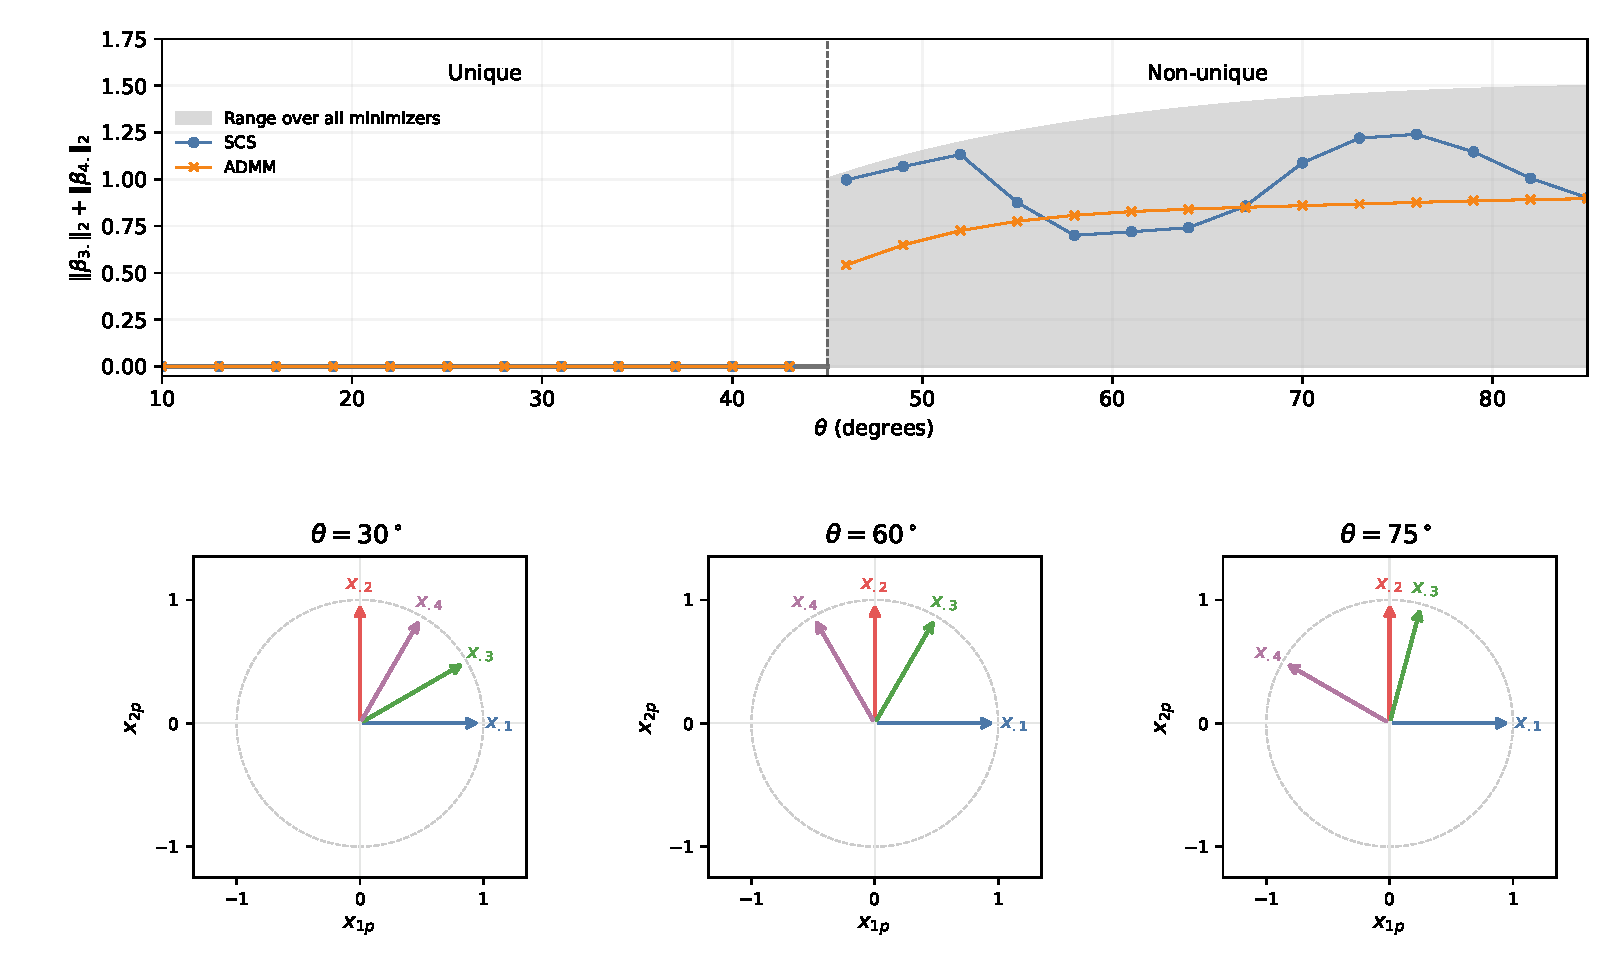
\includegraphics[width=\textwidth]{../figures/rotation_sweep/four_column_rotation_sweep.pdf}
\caption{Four-column rotation in Example~\ref{example:rotation_nonuniqueness}.
Top: total row norm assigned to the two added columns.
Shading gives its exact range over all minimizers; curves show SCS (scale $0.1$) and direct ADMM ($\rho=1$), both initialized at zero with absolute and relative tolerances $10^{-9}$.
Every optimum has loss $2$.
One added column coincides with a basis column at $\theta=\pi/4$; this angle is excluded from the scalar uniqueness claim and numerical sweep.
Bottom: dictionaries before and after the added columns bracket the $y$-axis.
Scalar basis pursuit remains unique on both open angle intervals.}
    \label{fig:rotation-nonuniqueness}
\end{figure}

\subsubsection{Failure of minimum-Frobenius support containment}
\label{sec:min_norm_support_failure}

The union of supports of all minimizers contains every orthonormal subset, but the numerical solver need not recover this union.
\citet{Tibshirani2012TheLP} proves minimum-$\ell_2$-norm selection for an extended least-angle regression algorithm for the Lasso, and \citet{Mishkin2023-yt} characterize minimum-norm group Lasso solutions.
We do not impose minimum-Frobenius selection; developing an algorithm that selects such a minimizer or recovers the union of supports is future work.
Even selecting the minimum-Frobenius minimizer does not ensure this containment (Example~\ref{example:min_norm_support_failure}).
We are not aware of a computationally efficient method for reliably recovering the union of supports at the scales considered here, although one may exist.
Our experiments evaluate the supports returned by the solver directly.
The empirical comparisons do not require minimum-Frobenius selection or recovery of the union of supports, and Figure~\ref{fig:optimizer_support_stability} checks support stability on selected real-data replicates.

\begin{example}
\label{example:min_norm_support_failure}
Let $D=2$, $P=10$, and
\begin{align}
u&=\begin{bmatrix}\sqrt3/2\\1/2\end{bmatrix}, &
v&=\begin{bmatrix}\sqrt3/2\\-1/2\end{bmatrix}, &
X&=[e_1,e_2,\underbrace{u,u,u,u}_{4},\underbrace{v,v,v,v}_{4}],
\end{align}
where $e_1,e_2$ are the standard basis vectors of $\mathbb R^2$.
All columns have unit length, so $n_q^{\times P}(X)=X$.
The matrix $\beta^{(0)}=[I_2\;0]^\top$ is a basis-pursuit minimizer supported on $\{1,2\}$.
However, the unique minimum-Frobenius basis-pursuit minimizer is
\begin{align}
\beta^*&=\operatorname{diag}(c^*)X^\top, &
c^*&=(0,2/3,1/6,1/6,1/6,1/6,1/6,1/6,1/6,1/6)^\top.
\end{align}
Thus $S(\beta^*)=\{2,\ldots,10\}$ does not contain the orthonormal subset $\{1,2\}$.
The weights $c_1=1/4$, $c_2=3/4$, and $c_3=\cdots=c_{10}=1/8$ give another minimizer with all ten rows nonzero.
\end{example}

\begin{proof}
For any feasible $\beta$, unit column lengths give
\begin{align}
2=\operatorname{tr}(X\beta)
=\sum_{p=1}^{10}\beta_{p.}x_{.p}
\leq\sum_{p=1}^{10}\|\beta_{p.}\|_2.
\end{align}
Since $\beta^{(0)}$ attains $2$, the minimum group norm is $2$.
Equality requires $\beta_{p.}=c_p x_{.p}^\top$ with $c_p\geq0$ for every $p$.
Hence every minimizer satisfies
\begin{align}
\sum_{p=1}^{10}c_p x_{.p}x_{.p}^\top=I_2,
\qquad \|\beta\|_F^2=\sum_{p=1}^{10}c_p^2.
\end{align}
The off-diagonal constraint gives $\sum_{p=3}^6c_p=\sum_{p=7}^{10}c_p$.
Write this common sum as $4s$.
The two diagonal constraints then give
\begin{align}
c_1=1-6s,\qquad c_2=1-2s,\qquad 0\leq s\leq1/6.
\end{align}
The repeated columns need not have equal coefficients.
Nevertheless, Cauchy--Schwarz gives
\begin{align}
\sum_{p=3}^6c_p^2\geq\frac{(4s)^2}{4}=4s^2,
\qquad
\sum_{p=7}^{10}c_p^2\geq4s^2,
\end{align}
with equality only when all coefficients within each group equal $s$.
Consequently every minimizer satisfies
\begin{align}
\|\beta\|_F^2
&\geq(1-6s)^2+(1-2s)^2+8s^2 \\
&=\frac23+48\left(s-\frac16\right)^2
\geq\frac23.
\end{align}
The matrix $\beta^*$ attains equality: $X\beta^*=I_2$, $\|\beta^*\|_{1,2}=2$, and $\|\beta^*\|_F^2=2/3$.
Equality forces $s=1/6$ and equal coefficients within both repeated groups, so $\beta^*$ is the unique minimum-Frobenius minimizer.
\end{proof}

\subsubsection{Proof of Proposition \ref{prop:D_min}}

\begin{restatedproposition}{prop:D_min}
$\ell (X_S) = D , |S| = D \Leftrightarrow X_S X_S^T = I_D$
\end{restatedproposition}

$X_S$ admits a QR decomposition $X_S = QR$ where $Q$ is orthogonal and $R$ is upper triangular.
By Proposition \ref{prop:basis_pursuit_selection_invariance}, we can assume without loss of generality that $Q = I_D$.
That is, $X_S$ is upper triangular.
Thus, $\beta = X_S^{-1}$ is upper triangular with diagonal elements $\beta_{dd} = R_{dd}^{-1}$.
$\|\beta_{d.}\|_2 \geq \beta_{dd}$, with equality only occurring when the off-diagonal elements are $0$.
Therefore, $\|\beta_{1,2}\| \geq D$ with equality occurring only when $\beta = I_D$.

\subsubsection{Proof of Proposition \ref{prop:loss_without_isometry}}

\begin{restatedproposition}{prop:loss_without_isometry}
Without $|S|=D$, $\ell(X_{.S})=D$ does not imply that $X_{.S}$ contains an orthonormal column-submatrix.
\end{restatedproposition}

\begin{proof}
For $D=2$, take the Mercedes-Benz frame
\begin{align}
X&=\begin{bmatrix}
0&\sqrt3/2&-\sqrt3/2\\
1&-1/2&-1/2
\end{bmatrix}, &
\beta&=\frac23 X^\top.
\end{align}
Its columns have unit length, so $n_q^{\times P}(X)=X$, and $XX^\top=\frac32 I_2$ gives $X\beta=I_2$ and $\|\beta\|_{1,2}=3\cdot\frac23=2=D$.
For every feasible $B$, $2=\operatorname{tr}(XB)=\sum_{p=1}^3\langle X_{.p},B_{p.}^\top\rangle \leq\sum_{p=1}^3\|B_{p.}\|_2$, so $\ell(X)=D$.
Every pair of distinct columns has inner product $-1/2$, so no pair is orthonormal.
\end{proof}

\subsubsection{Proof of Proposition \ref{prop:computational_complexity}}
\label{proof:computational_complexity}

\begin{restatedproposition}{prop:computational_complexity}
The computational complexity of each step of Isometry Pursuit is $O(D^2P)$.
\end{restatedproposition}

% TODO: Replace the direct-ADMM derivation below with the SCS cached linear-solve and cone-projection analysis for the runtime panel of Figure 3, distinguishing setup from per-iteration work.
\begin{proof}
The augmented split Lagrangian minimized by ADMM is
    \begin{align}
    \mathcal L_{\rho,\gamma, \nu} (X,\beta,z) = \|z\|_{1,2} + \text{tr}(\nu^T (I_D - n_q^{\times P}(X) \beta)) + \rho \|I_D - n_q^{\times P}(X) \beta\|_F^2 + \gamma \|\beta - z\|_F^2
    \end{align}
This minimization problem is
    \begin{align}
        \arg \min_{\beta,z \in P \times D} \mathcal L_{\rho,\gamma,\nu} (X,\beta,z)
    \end{align}
For a more detailed explanation of the reasons to prefer optimizing the split augmented Lagrangian over direct optimization of Equation \ref{prog:isometry_pursuit} see \citet{Boyd2010-jd}.
    
The three main subroutines ( \ref{eq:beta_update} - \ref{eq:nu_update}) called by ADMM determine the per iteration complexity.
The update rules of the ADMM algorithm used to optimize the augmented split Lagrangian are
    \begin{align}
    \beta^{k+1} = \arg \min_{\beta \in P \times D} \mathcal L_{\rho,\gamma,\nu} (X,\beta,z^k) \\
    z^{k+1} = \arg \min_{z \in P \times D} \mathcal L_{\rho,\gamma,\nu} (X,\beta^{k+1},z) \\
    \nu^{k+1} = \nu^k + \rho (I_D - n_q^{\times P}(X) \beta^{k+1})
    \end{align}
We will analyze the computational complexity of each of these steps by rewriting the update rules according to the specifics of the isometry pursuit problem.

The beta update Equation \ref{eq:beta_update} projects the solution onto the feasible set.
\begin{align}
    \label{eq:beta_update}
    \beta^{k+1} &= \arg \min_{\beta \in P \times D}  \text{tr}({\nu^k}^T (I_D - n_q^{\times P}(X) \beta)) + \rho \|I_D - n_q^{\times P}(X) \beta\|_2^2 + \gamma \|\beta - z^k\|_2^2 \\
    &= (\rho \, n_q^{\times P}(X)^T n_q^{\times P}(X) + \gamma I_P)^{-1} (\rho \, n_q^{\times P}(X)^T I_D + \gamma z^k + n_q^{\times P}(X)^T \nu^k)
    \end{align}
% This is accomplished through computation of the pseudo-inverse of the linear regression solution $(n_q^{\times P}(X)^T n_q^{\times P}(X))^{-1} n_q^{\times P}(X)^T I_D$.
Write $N=n_q^{\times P}(X)$.
The Woodbury identity gives
\begin{align}
(\gamma I_P+\rho N^\top N)^{-1}
=\gamma^{-1}\left[I_P-\rho N^\top
(\gamma I_D+\rho NN^\top)^{-1}N\right].
\end{align}
For fixed $N$, $\rho>0$, and $\gamma>0$, forming $NN^\top$ and factoring $\gamma I_D+\rho NN^\top$ costs $O(PD^2+D^3)$ once.
To apply the inverse to a $P\times D$ right-hand side $R$, compute $NR$, solve $(\gamma I_D+\rho NN^\top)Z=NR$ using the cached factorization, and return $\gamma^{-1}(R-\rho N^\top Z)$.
The two matrix products cost $O(PD^2)$ and the solve costs $O(D^3)$.
Forming the right-hand side of the coefficient update also costs $O(PD^2)$, so the per-iteration cost is $O(PD^2)$ when $P\geq D$.

Subsequently, the z update Equation \ref{eq:z_update} is soft-thresholding operation onto a contracted level set $\|\|_{1,2}$ ball.
\begin{align}
    \label{eq:z_update}
    z^{k+1} &= \arg \min_{z \in P \times D} \|z\|_{1,2} + \gamma \|z - \beta^{k+1}\|_2^2 \\
    &= \begin{cases} (1 - \frac{1}{\gamma\|\beta_{j.}^{k+1}\|_2}) (\beta_{j.}^{k+1}) \; \text{if} \; \|\beta_{j.}^{k+1}\|_2 > \frac{1}{\gamma}\\
        0 \; \text{otherwise}
    \end{cases}
\end{align}
The computational complexity of this operation is $O(PD)$.

Finally, the $\nu$ update Equation \ref{eq:nu_update} increases the squeezing of the $z$ and $\beta$ variables towards to each other.
\begin{align}
\nu^{k+1} = \nu^k + \rho (I_D - n_q^{\times P}(X) \beta^{k+1})
\label{eq:nu_update}
\end{align}
In this step, the dual variable $\nu$ that controls the penalty accrued by the splitting is updated in the direction of the constraint violation.
The computational complexity of this operation is dominated by that of the matrix multiplication $n_q^{\times P}(X) \beta^{k+1}$.
That is, it is $O(D^2P)$.
\end{proof}

\subsection{Partial derivatives of candidate losses}
\label{sec:loss_derivatives}

We summarize the column-wise derivatives of the losses in Table \ref{tab:loss_functions}.
Throughout this section let $X = [x_1,\dotsc,x_D] \in \mathbb R^{D \times D}$ be full rank.
For a scalar loss $L(X)$, write
\begin{align}
\nabla_X L = \left[
\frac{\partial L}{\partial x_1},
\dotsc,
\frac{\partial L}{\partial x_D}
\right].
\end{align}
All formulas are stated on smooth strata: rank deficient matrices, repeated singular values, and zero rows of pseudoinverse factors should be handled using subgradients.

We will use two common identities.
First, if $X = U \operatorname{diag}(\sigma) V^\top$ is a singular value decomposition and $L(X) = \sum_{d=1}^D \phi(\sigma_d(X))$, then
\begin{align}
\nabla_X L = U \operatorname{diag}(\phi'(\sigma_1),\dotsc,\phi'(\sigma_D)) V^\top .
\label{eq:spectral_gradient_identity}
\end{align}
Second, for normalized losses let $N = n_q^{\times D}(X)$.
If $M = \nabla_N L$, then the column-wise chain rule is
\begin{align}
\frac{\partial L}{\partial x_p} = \mathrm{D}n_q(x_p)^\top M_{.p}.
\label{eq:column_chain_rule}
\end{align}
For $r=\|x\|_2$, write $n_q(x)=s(r)x$ with $s(r)=q(r)/r$.
Then
\begin{align}
\mathrm{D}n_q(x) &= s(r) I_D + \frac{s'(r)}{r}xx^\top, \\
s'(r) &= \frac{q'(r)}{r} - \frac{q(r)}{r^2}, \\
q'(r) &= -\frac{2e(e^r-r^{-2}e^{1/r})}{(e^r+e^{1/r})^2}.
\label{eq:normalization_jacobian}
\end{align}
Since $\mathrm{D}n_q(x)$ is symmetric, the transpose in this chain rule may be omitted.

\paragraph{Distortion.}
Let $\sigma_1=\sigma_{\max}(X)$ and $\sigma_D=\sigma_{\min}(X)$ with corresponding singular vectors $u_1,v_1$ and $u_D,v_D$.
For
\begin{align}
L_{\mathrm{dist}}(X)=\frac{\sigma_1}{\sigma_D}-1,
\end{align}
The spectral gradient identity gives
\begin{align}
\nabla_X L_{\mathrm{dist}}
= \frac{u_1v_1^\top}{\sigma_D}
- \frac{\sigma_1}{\sigma_D^2}u_Dv_D^\top .
\end{align}
The derivative is insensitive to uniform rescaling, which is the sense in which this loss does not prefer unit length.

\paragraph{Isometry loss.}
For
\begin{align}
L_{\mathrm{iso}}(X)=\sum_{d=1}^D g(\sigma_d(X))-D,
\end{align}
we have
\begin{align}
g'(t) = \frac{e^t - t^{-2}e^{1/t}}{2e}.
\end{align}
Thus
\begin{align}
\nabla_X L_{\mathrm{iso}}
= U \operatorname{diag}(g'(\sigma_1),\dotsc,g'(\sigma_D))V^\top .
\end{align}

\paragraph{S-divergence to identity.}
Let $G=X^\top X$ and
\begin{align}
L_{\mathrm{sdiv}}(X)
= \log\det\left(\frac{G+I_D}{2}\right)
-\frac{1}{2}\log\det(G).
\end{align}
The constant $\log\det(1/2)$ does not contribute to the derivative.
Using $d\log\det A = \operatorname{tr}(A^{-1}dA)$ and $dG=dX^\top X+X^\top dX$,
\begin{align}
\nabla_X L_{\mathrm{sdiv}}
= 2X(G+I_D)^{-1} - XG^{-1}.
\end{align}

\paragraph{Normalized log-det volume.}
Let $N=n_q^{\times D}(X)$ and
\begin{align}
L_{\mathrm{nld}}(X)= -\sum_{d=1}^D \log\sigma_d(N).
\end{align}
For square full-rank $N$, this is $-\log|\det N|$, so
\begin{align}
\nabla_N L_{\mathrm{nld}} = -N^{-\top}.
\end{align}
Therefore, by the column-wise chain rule,
\begin{align}
\frac{\partial L_{\mathrm{nld}}}{\partial x_p}
= -\mathrm{D}n_q(x_p)^\top (N^{-\top})_{.p}.
\end{align}

\paragraph{Frobenius pseudoinverse.}
Let $N=n_q^{\times D}(X)$ and $B=N^{-1}$.
For
\begin{align}
L_{\mathrm{frob}}(X)=\|N^{-1}\|_F-\sqrt{D},
\end{align}
the differential identity $dB=-B(dN)B$ gives
\begin{align}
\nabla_N L_{\mathrm{frob}}
= -\frac{N^{-\top}N^{-1}N^{-\top}}{\|N^{-1}\|_F}.
\end{align}
Thus
\begin{align}
\frac{\partial L_{\mathrm{frob}}}{\partial x_p}
= \mathrm{D}n_q(x_p)^\top
\left(
-\frac{N^{-\top}N^{-1}N^{-\top}}{\|N^{-1}\|_F}
\right)_{.p}.
\end{align}

\paragraph{Isometry pursuit proxy.}
Let $N=n_q^{\times D}(X)$ and $B=N^{-1}$.
The differentiable proxy for the \isometrypursuit~ table row is
\begin{align}
L_{\mathrm{ip}}(X)=\|N^{-1}\|_{1,2}-D.
\end{align}
Define $R \in \mathbb R^{D\times D}$ by
\begin{align}
R_{p.}=\frac{B_{p.}}{\|B_{p.}\|_2}.
\end{align}
Then $R \in \partial \|B\|_{1,2}$ on the smooth stratum where every row of $B$ is nonzero, and
\begin{align}
\nabla_N L_{\mathrm{ip}} = -B^\top R B^\top.
\end{align}
The column-wise gradient is therefore
\begin{align}
\frac{\partial L_{\mathrm{ip}}}{\partial x_p}
= \mathrm{D}n_q(x_p)^\top (-B^\top R B^\top)_{.p}.
\end{align}

\newpage

\subsection{Additional experimental results}
\label{sec:additional_experimental_results}

\begin{figure}[t]
    \centering
    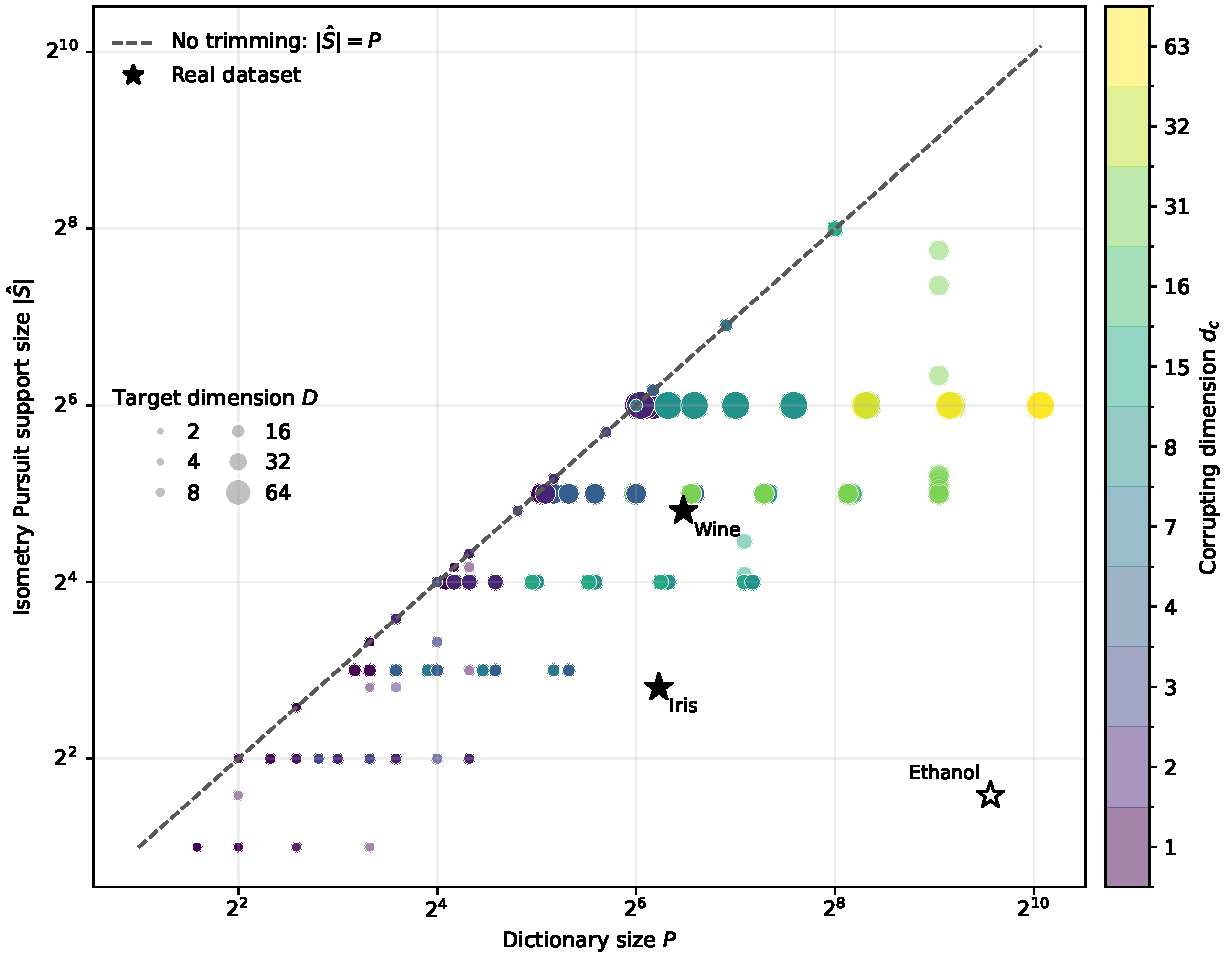
\includegraphics[width=0.82\textwidth]{../figures/synthetic_support_vs_dictionary.pdf}
\caption{Dictionary size $P$ versus the support size returned by \isometrypursuit.
Point area encodes target dimension $D$ and color encodes corrupting dimension $d_c$.
The dashed diagonal denotes no trimming.
Most runs lie below the diagonal, and the horizontal bands at $|\widehat S|=D$ show settings where \isometrypursuit~alone reduces the dictionary to the target cardinality.}
    \label{fig:synthetic-support-size}
\end{figure}

\begin{figure}[t]
    \centering
    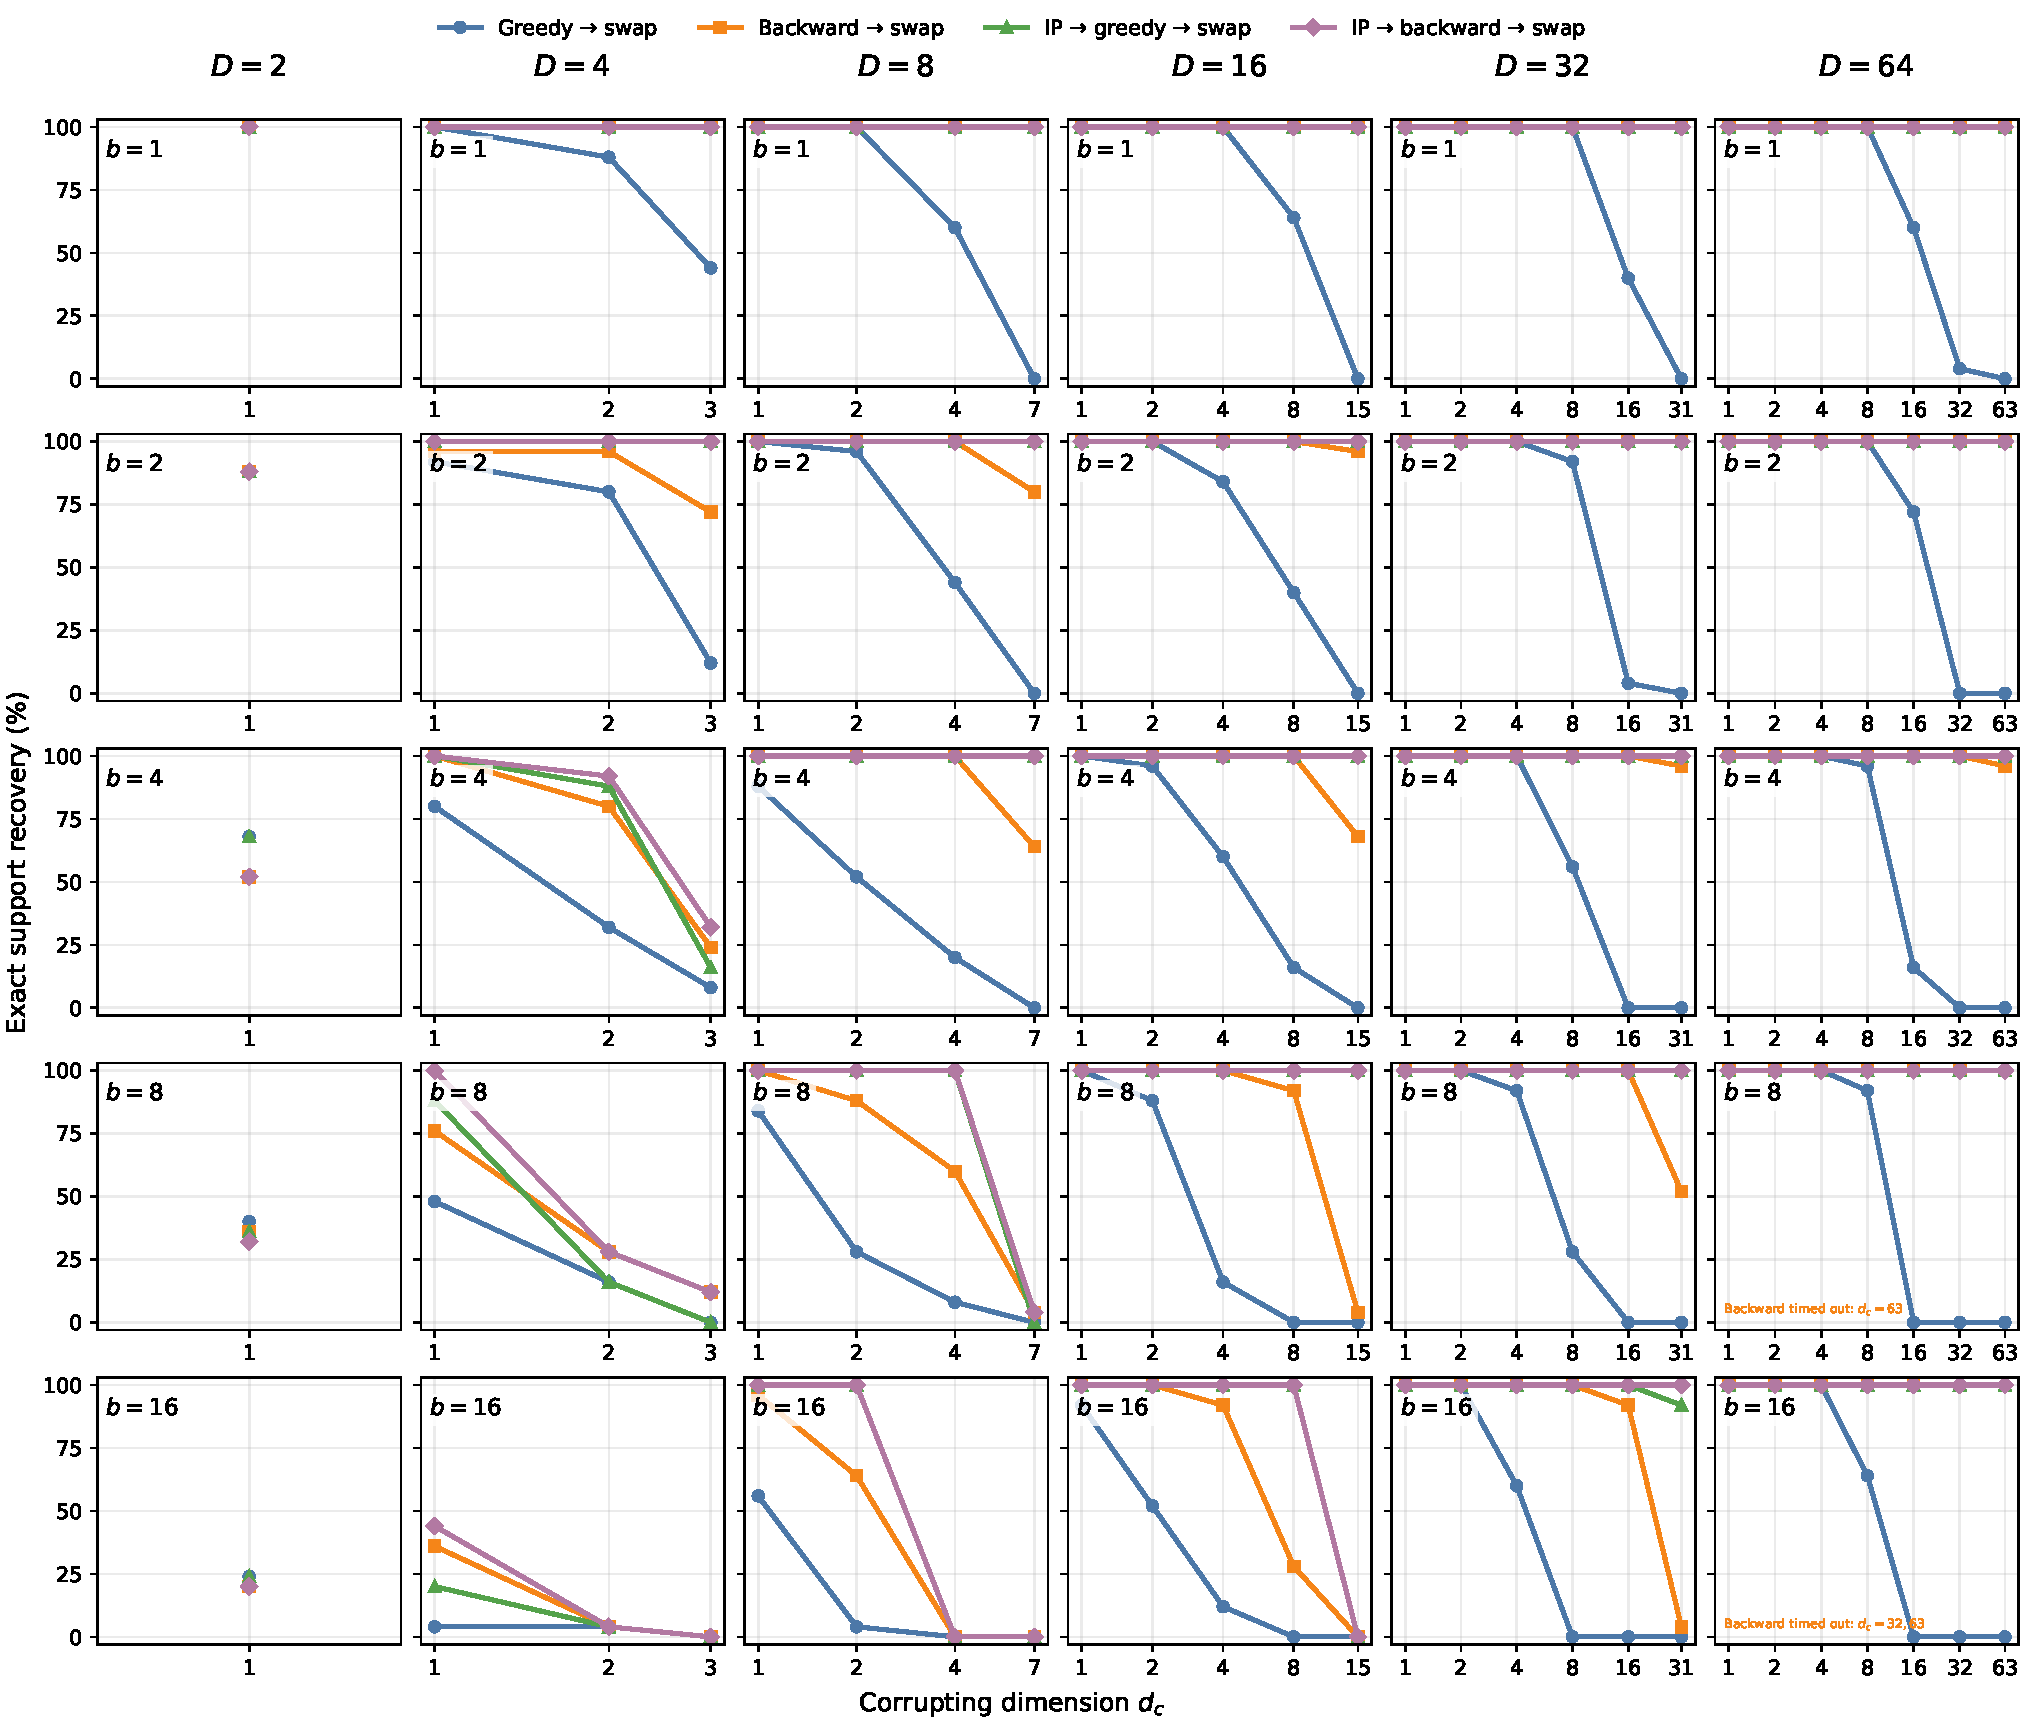
\includegraphics[width=\textwidth]{../figures/synthetic_support_recovery_grid.pdf}
\caption{Exact support recovery in the synthetic identity-block experiments.
Columns give target dimension $D$, rows give the number $b$ of corrupting matrices, and the horizontal axis gives their dimension $d_c$.
Each point is the percentage of 25 replicates for which the selected support equals the planted $D$-column identity block.
Faint dashed curves toward an off-axis value of $-100$ mark settings omitted by the backward-search work budget; they are not recovery measurements.}
    \label{fig:synthetic-support-recovery}
\end{figure}

\begin{table}[t]
\centering
\small
\resizebox{\textwidth}{!}{%
\begin{tabular}{lccc}
\toprule
Method & Wine ($P=89$) & Iris ($P=75$) & Ethanol ($P=756$) \\
\midrule
Greedy $\rightarrow$ swap
    & $24.0\%\;/\;3.239$ & $60.0\%\;/\;0.179$
    & $84.0\%\;/\;0.0188$ \\
Backward $\rightarrow$ swap
    & $72.0\%\;/\;0.605$ & $88.0\%\;/\;0.0170$
    & $96.0\%\;/\;0.00330$ \\
\isometrypursuit $\rightarrow$ greedy $\rightarrow$ swap
    & \makecell{$40.0\%\;/\;2.446$\\$26.2/89\;(29.4\%)$}
    & \makecell{$56.0\%\;/\;0.0814$\\$6.72/75\;(9.0\%)$}
    & \makecell{$64.0\%\;/\;0.0180$\\$2.80/756\;(0.37\%)$} \\
\isometrypursuit $\rightarrow$ backward $\rightarrow$ swap
    & \makecell{$64.0\%\;/\;0.615$\\$26.2/89\;(29.4\%)$}
    & \makecell{$64.0\%\;/\;0.0545$\\$6.72/75\;(9.0\%)$}
    & \makecell{$64.0\%\;/\;0.0180$\\$2.80/756\;(0.37\%)$} \\
\bottomrule
\end{tabular}
}
\caption{Oracle attainment and regret for the four discrete-search pipelines.
Each entry is $\widehat P(\mathcal R_{m,r}=0)\;/\;\overline{\mathcal R}_m$: the percentage of replicates on which the method wins or ties for the lowest loss among the four methods, followed by its mean oracle regret.
For the two \isometrypursuit~pipelines, the second line reports $\overline{|\widehat S_{IP}|}/P$ and the corresponding retained percentage.
Losses within $10^{-9}$ are treated as ties.
Each dataset contains 25 replicates.
Because loss scales differ across datasets, regret magnitudes should be compared within columns.}
\label{tab:oracle-regret}
\end{table}

\clearpage
\begin{figure}[t]
    \centering
    \begin{subfigure}[t]{\textwidth}
        \centering
        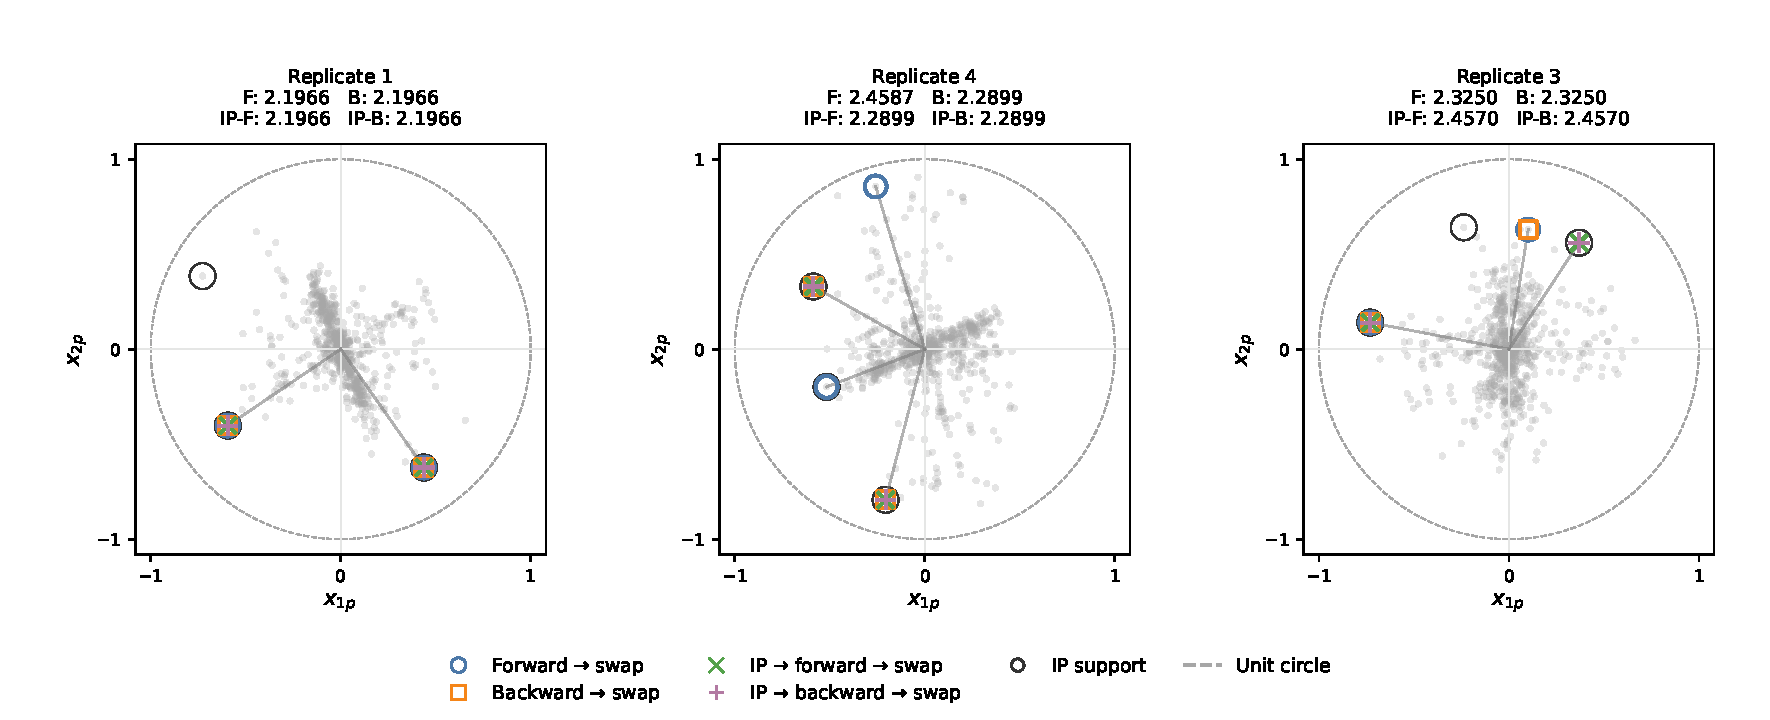
\includegraphics[width=\linewidth]{../figures/selection_examples/ethanol_selection_examples.pdf}
\caption{Ethanol tangent-space dictionaries.}
    \end{subfigure}
\par\medskip
    \begin{subfigure}[t]{\textwidth}
        \centering
        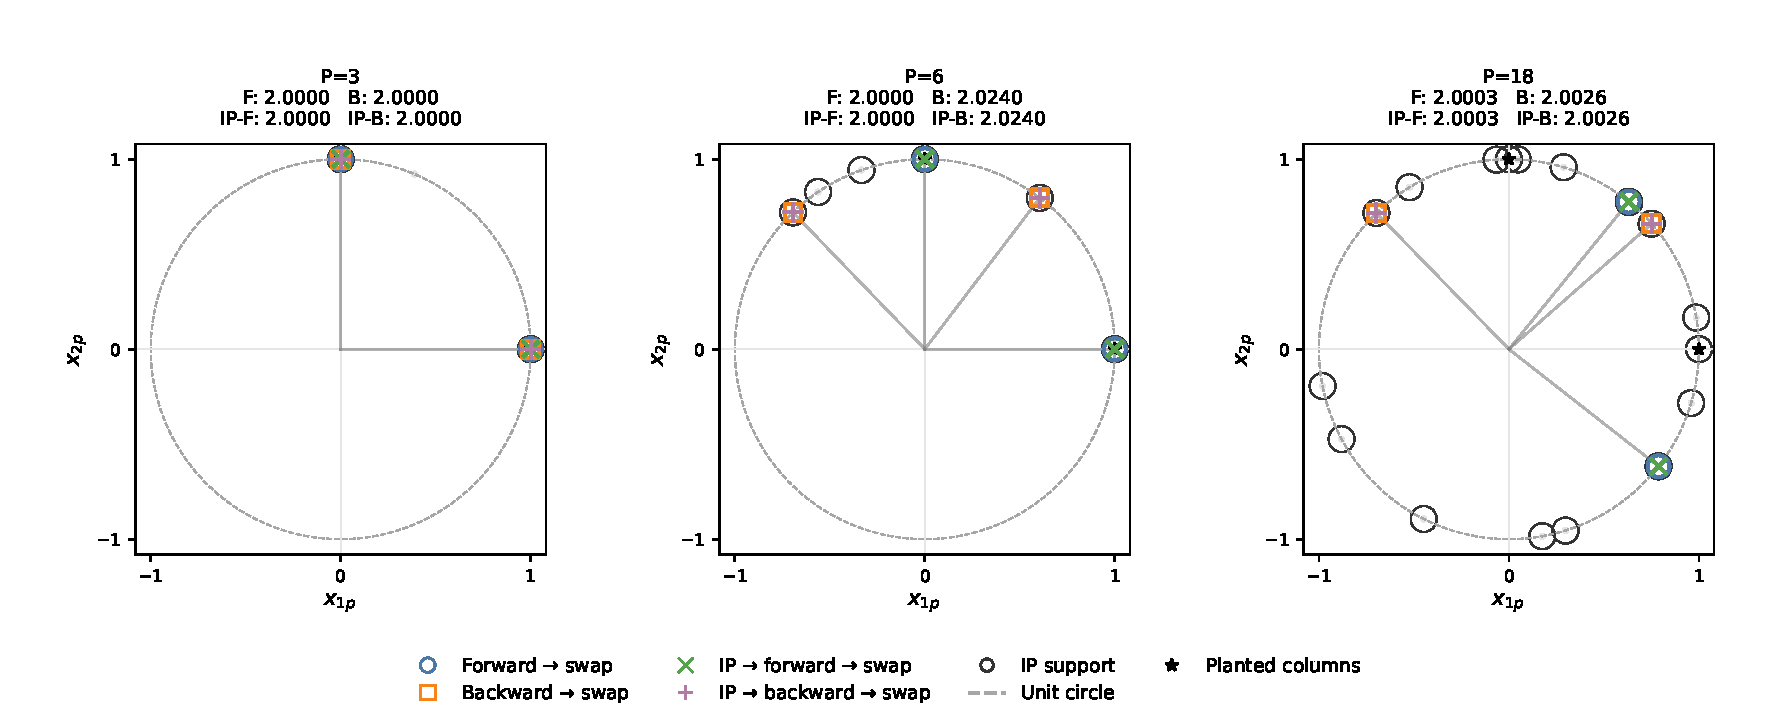
\includegraphics[width=\linewidth]{../figures/selection_examples/synthetic_selection_examples.pdf}
\caption{Synthetic identity-block dictionaries.}
    \end{subfigure}
\caption{Selections by the four search methods on $D=2$ dictionaries.
Each panel overlays all four methods on the original column coordinates.
Black rings mark the \isometrypursuit~support; colored markers show the final selected pairs, with overlapping markers indicating shared selections.
Gray lines connect selected columns to the origin, and the dashed circle marks unit length.
F and B denote forward and backward initialization, respectively; all four methods include swap refinement.
The reported losses are evaluated after column normalization.
(a) The first saved Ethanol examples where screening leaves the forward loss unchanged, improves it, and worsens it (replicates 1, 4, and 3).
(b) The first synthetic replicate with 1, 4, and 16 added one-dimensional blocks; stars mark the planted orthonormal pair.
These are illustrative examples from the saved experiments.}
    \label{fig:selection-examples}
\end{figure}

\subsection{Sparsity versus iteration count}
\label{sec:sparsity_iterations}

We compare independently initialized SCS solves at iteration limits from $1$ to $25{,}000$ on the same $25$ replicates of each real dataset.
We fix the SCS scale at $0.1$, disable adaptive scaling and acceleration, and set absolute and relative tolerances to $10^{-12}$.
We zero coefficient entries below $10^{-6}$ in magnitude and retain rows with norm above $10^{-4}$.
Figure~\ref{fig:sparsity_iterations} shows the retained fraction and exact agreement with the saved reference supports.
For all subsequent tested limits, every Wine replicate matches its reference support from $100$ iterations onward, every Iris replicate from $1{,}000$, and every Ethanol replicate from $2{,}500$.
These observations concern thresholded numerical supports, rather than a guarantee of finite support identification.

\begin{figure}[t]
\centering
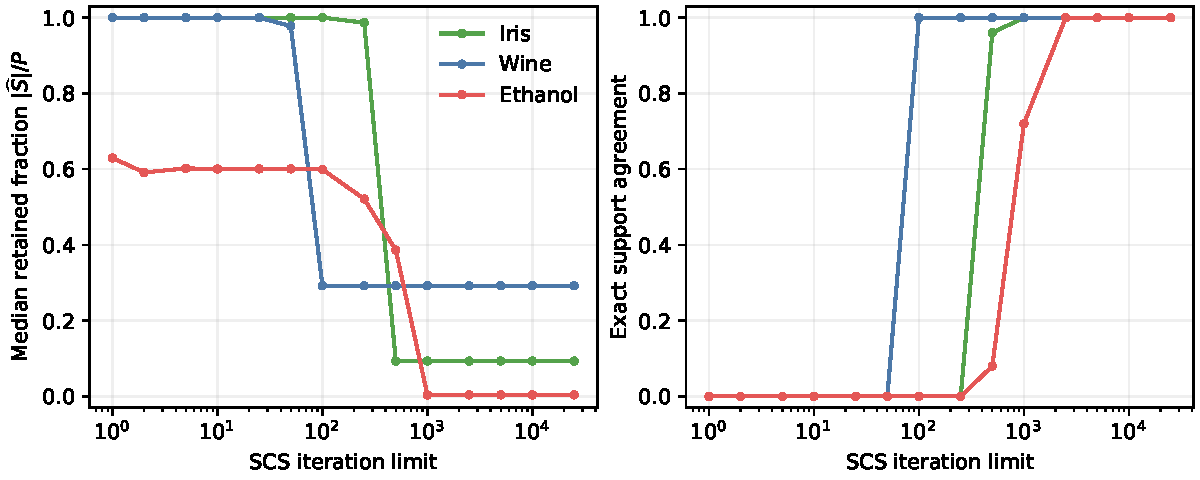
\includegraphics[width=\textwidth]{../figures/scs_early_stop/sparsity_iterations.pdf}
\caption{Sparsity as a function of the SCS iteration limit on Iris, Wine, and Ethanol.
The left panel shows the median retained fraction across $25$ replicates per dataset; the right panel shows the fraction matching the saved reference support exactly.
Each point summarizes independent cold starts at the indicated limit; the solver may terminate before reaching that limit.}
\label{fig:sparsity_iterations}
\end{figure}

\subsection{Sensitivity to optimizer settings}
\label{sec:optimizer_sensitivity}

We fix the first replicate from each real dataset and compare SCS scales and direct ADMM parameters $\rho\in\{0.01,0.1,1,10,100\}$, initializing both optimizers at zero.
Direct ADMM alternates projection onto $N\beta=I_D$, rowwise soft thresholding, and a scaled dual update.
We set absolute and relative solver tolerances to $10^{-8}$ and allow $10^5$ iterations, with a 25-second solve limit.
We zero coefficient entries with magnitude below $10^{-6}$ and retain rows with norm above $10^{-4}$.
For the three Ethanol SCS settings that reach the iteration limit, we also run up to $5\times10^5$ iterations with a 240-second limit.
These checks use the saved input matrices and do not rerun the main experiments.

For the large synthetic cases, we freeze the first replicate of each of the $65$ conditions at $D=32,64$ and compare both solvers at the same five parameter values, giving $650$ solver runs.
Both start at zero, with absolute and relative tolerances $10^{-8}$, at most $5\times10^5$ iterations, and a 240-second solve limit.
We use SCS at scale $0.1$ in the main large-case comparison: it converges on all $65$ matrices and has the lowest total runtime among the tested SCS settings.
Separate Lambda tasks then run the greedy searches on the saved matrices and supports.
Full-dictionary searches are shared across optimizer settings; identical candidate supports also share a search.
The search seed is the original simulation seed.
These unit-column dictionaries are scored using $\|(X_{.S})^\dagger\|_{1,2}$, where $\dagger$ denotes the Moore--Penrose pseudoinverse, rather than solving basis pursuit at each deletion.
The initial search batch uses a 240-second limit and a $10^9$ backward-initialization work budget.
We rerun all 28 searches excluded by that work budget without an arithmetic cutoff, using a 245.37-second limit equal to the longest observed IP runtime.
Of these, 23 complete and five reach the time limit: four during backward elimination and one during swap refinement.
We rerun the last case with the cutoff applied only to initialization; elimination takes 208.9 seconds and swaps take 36.7 seconds, giving 24 completed replacements and four capped initializers.
Figure~\ref{fig:synthetic-ground-truth-regret} includes completed replacements for SCS at scale $0.1$; Figure~\ref{fig:complexity-runtime-early-stop} also includes capped backward initializers.
There is no additional column-count limit.
All large-case solver and search timings use 3072 MB Lambda workers; the smaller-case and real-data timings are local.
Figure~\ref{fig:optimizer_parameter_sweep} includes final searches from all ten settings, including settings whose solver reached a limit.

\begin{figure}[t]
\centering
\begin{subfigure}[t]{0.49\textwidth}
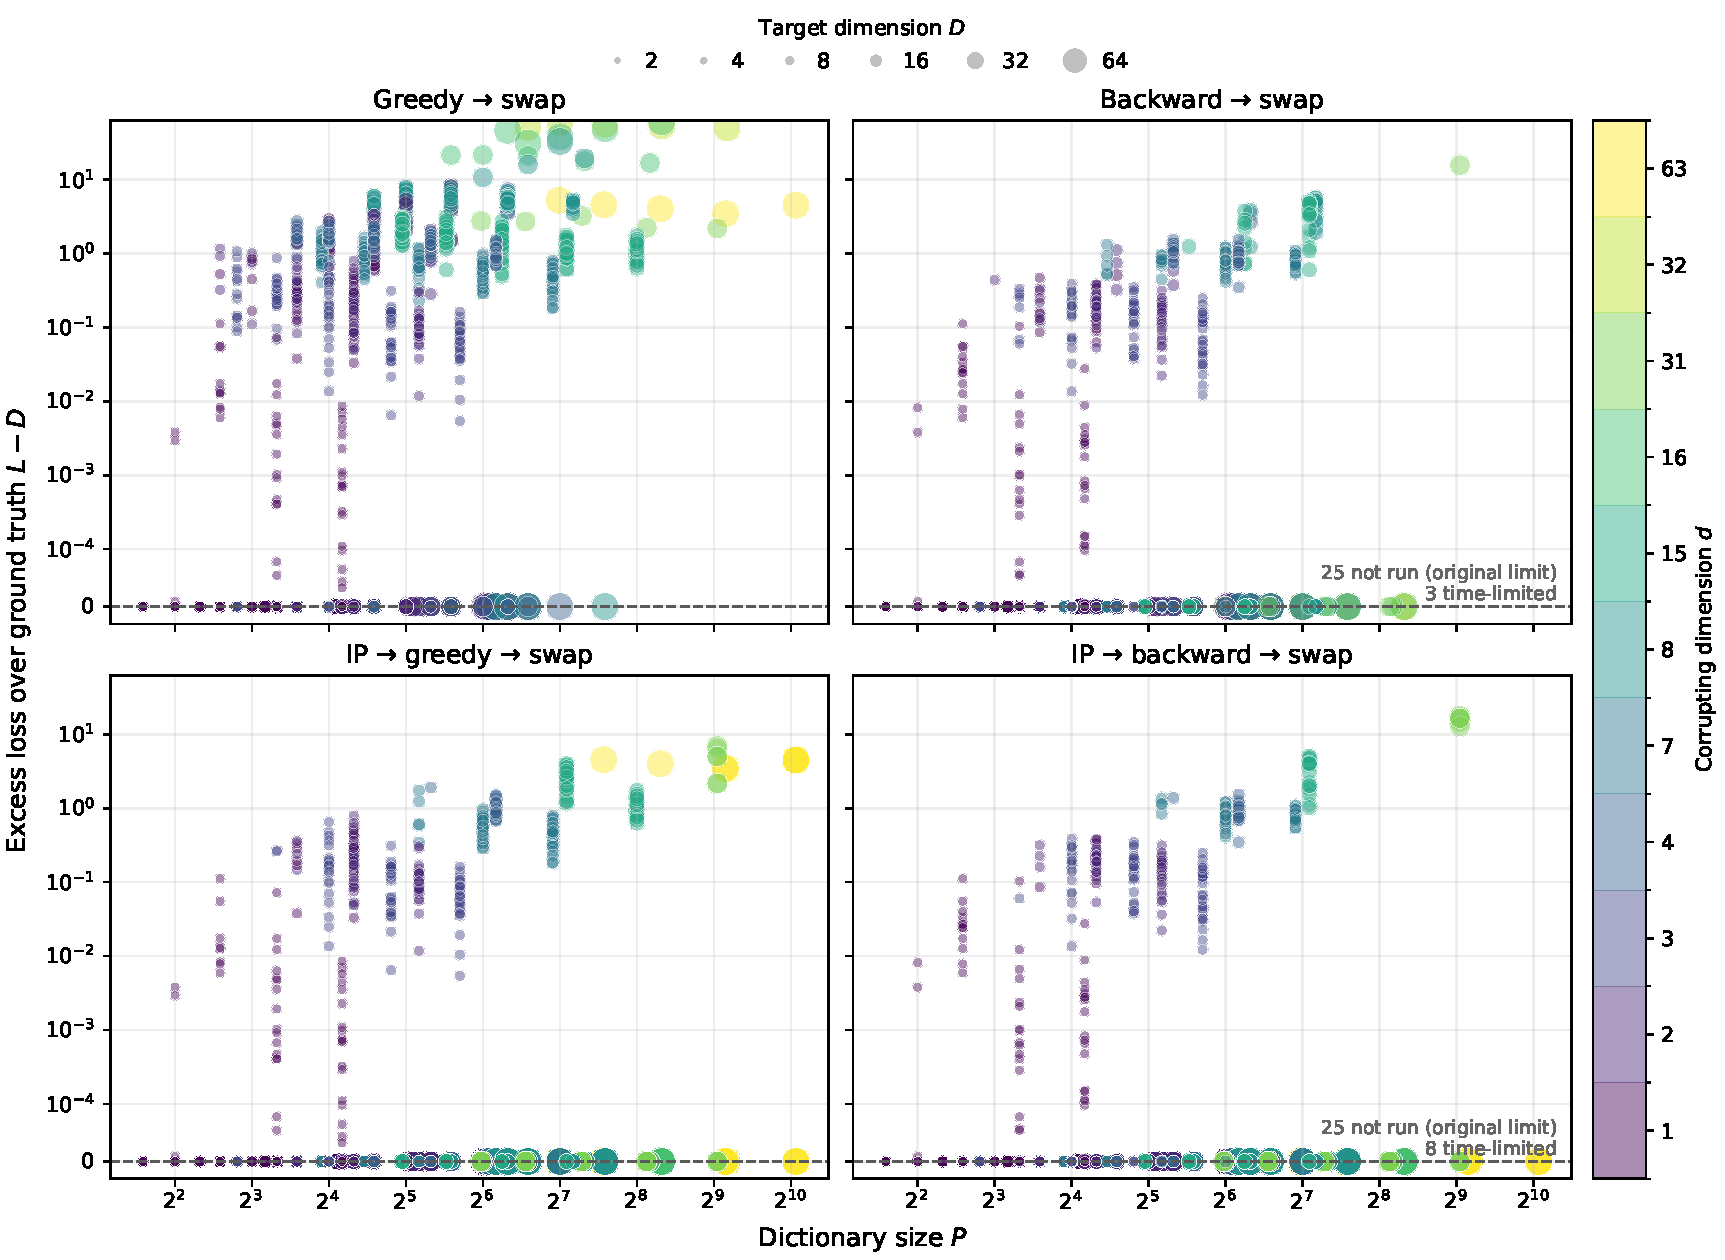
\includegraphics[width=\linewidth]{../figures/optimizer_parameter_sweep/synthetic_regret_all_settings.pdf}
\caption{Ground-truth regret across optimizer settings.}
\end{subfigure}\hfill
\begin{subfigure}[t]{0.49\textwidth}
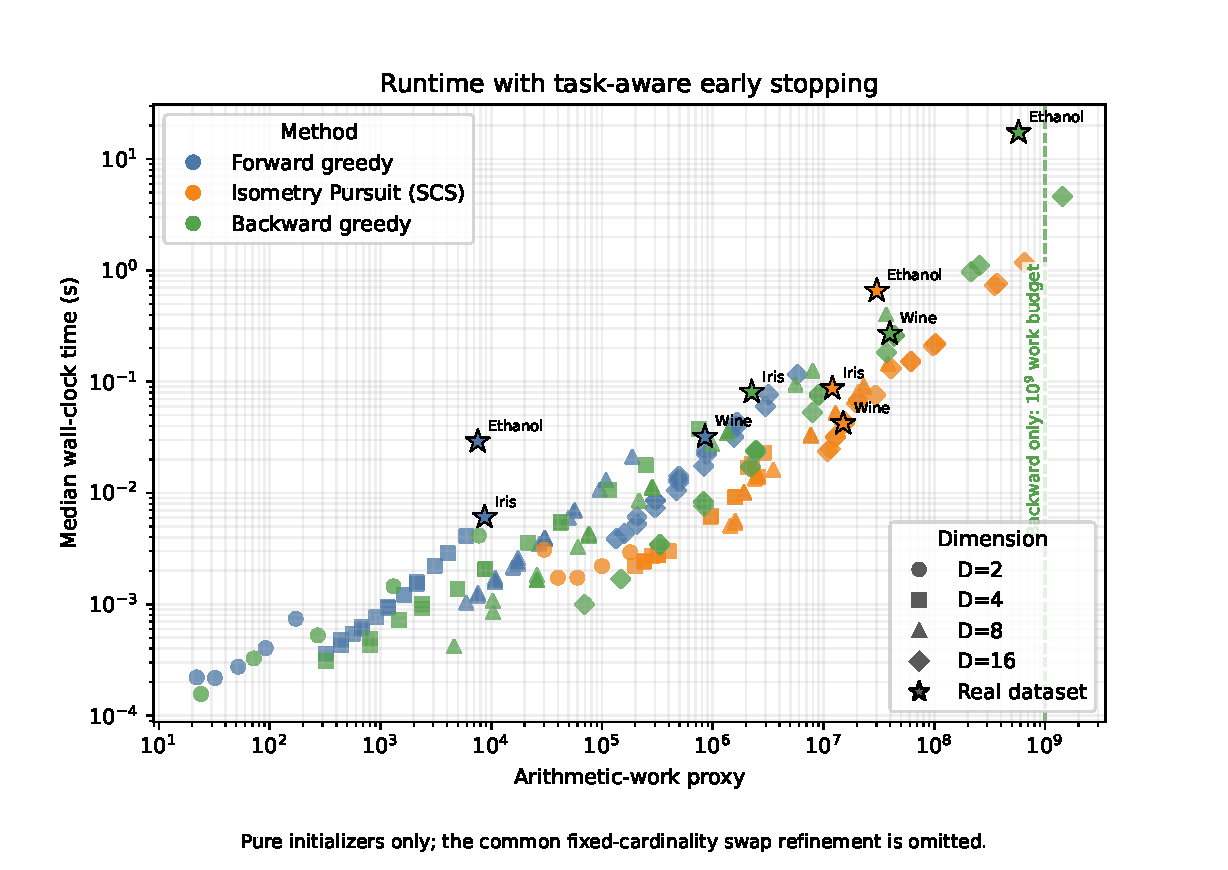
\includegraphics[width=\linewidth]{../figures/complexity_runtime/complexity_vs_runtime_overlay_with_early_stopping.pdf}
\caption{Arithmetic work versus runtime.}
\end{subfigure}
\caption{Full parameter comparison for the synthetic cloud experiments.
At $D=32,64$, we compare SCS scales and ADMM parameters in $\{0.01,0.1,1,10,100\}$ on the same fixed matrices.
Full-dictionary searches are shared across settings; smaller dimensions use the original replicates.
The runtime panel shows pure initializers, with swaps omitted; large-case timings are from Lambda and other timings are local.
Work for SCS and ADMM is the observed iteration count times $D^2P$, which does not distinguish their per-iteration constants.
Open markers denote capped runs; capped backward points show elapsed time against the work required for full elimination.
The dashed line marks the longest observed cloud IP runtime.}
\label{fig:optimizer_parameter_sweep}
\end{figure}

\begin{figure}[t]
    \centering
    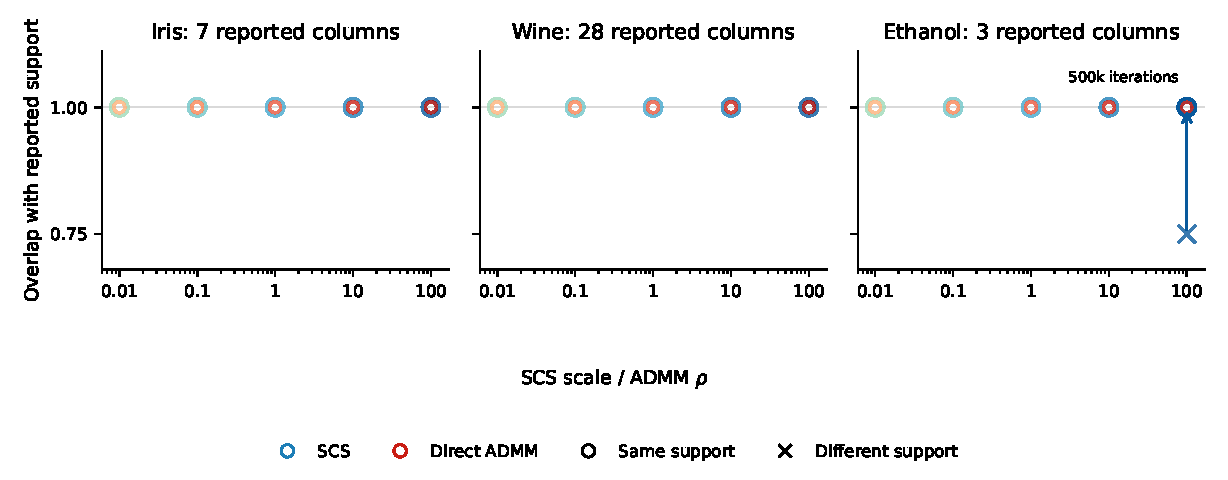
\includegraphics[width=\textwidth]{../figures/optimizer_support_stability.pdf}
\caption{Support stability on one fixed replicate from each real dataset.
We compare each retained support $S$ with its originally reported support $S_0$ using $|S\cap S_0|/|S\cup S_0|$.
SCS uses a green--blue color map and direct ADMM an orange--red color map; darker shades denote larger parameters.
Circles indicate identical supports and crosses indicate a difference.
Iris and Wine retain the same 7 and 28 columns, respectively, in all ten settings.
Nine initial Ethanol settings retain the same 3 columns; SCS at scale 100 initially retains one extra column, which disappears in the longer run (arrow).
The Ethanol SCS runs at scales 0.1, 10, and 100 reach their iteration limit even in the longer runs and are included here.
This is a stability check on the selected replicates, not a support-recovery guarantee.}
    \label{fig:optimizer_support_stability}
\end{figure}

\subsection{Support cardinalities}
\label{sec:support_cardinalities}

Figure~\ref{fig:support_cardinalities} reports the distribution of retained candidate-dictionary sizes $|\widehat{S}_{IP}|$ across the real-data replicates.
While typically $|\widehat{S}_{IP}| << P$, there are cases for Ethanol where this is not the case that drive up the means.
Further investigation into the extreme failure of isometry pursuit to sparsify in the the minor chunk of the bimodal Ethanol support cardinality distribution is warranted.

\begin{figure}[t]
    \centering
    % Wine
    \begin{subfigure}[b]{0.32\textwidth}
        \centering
        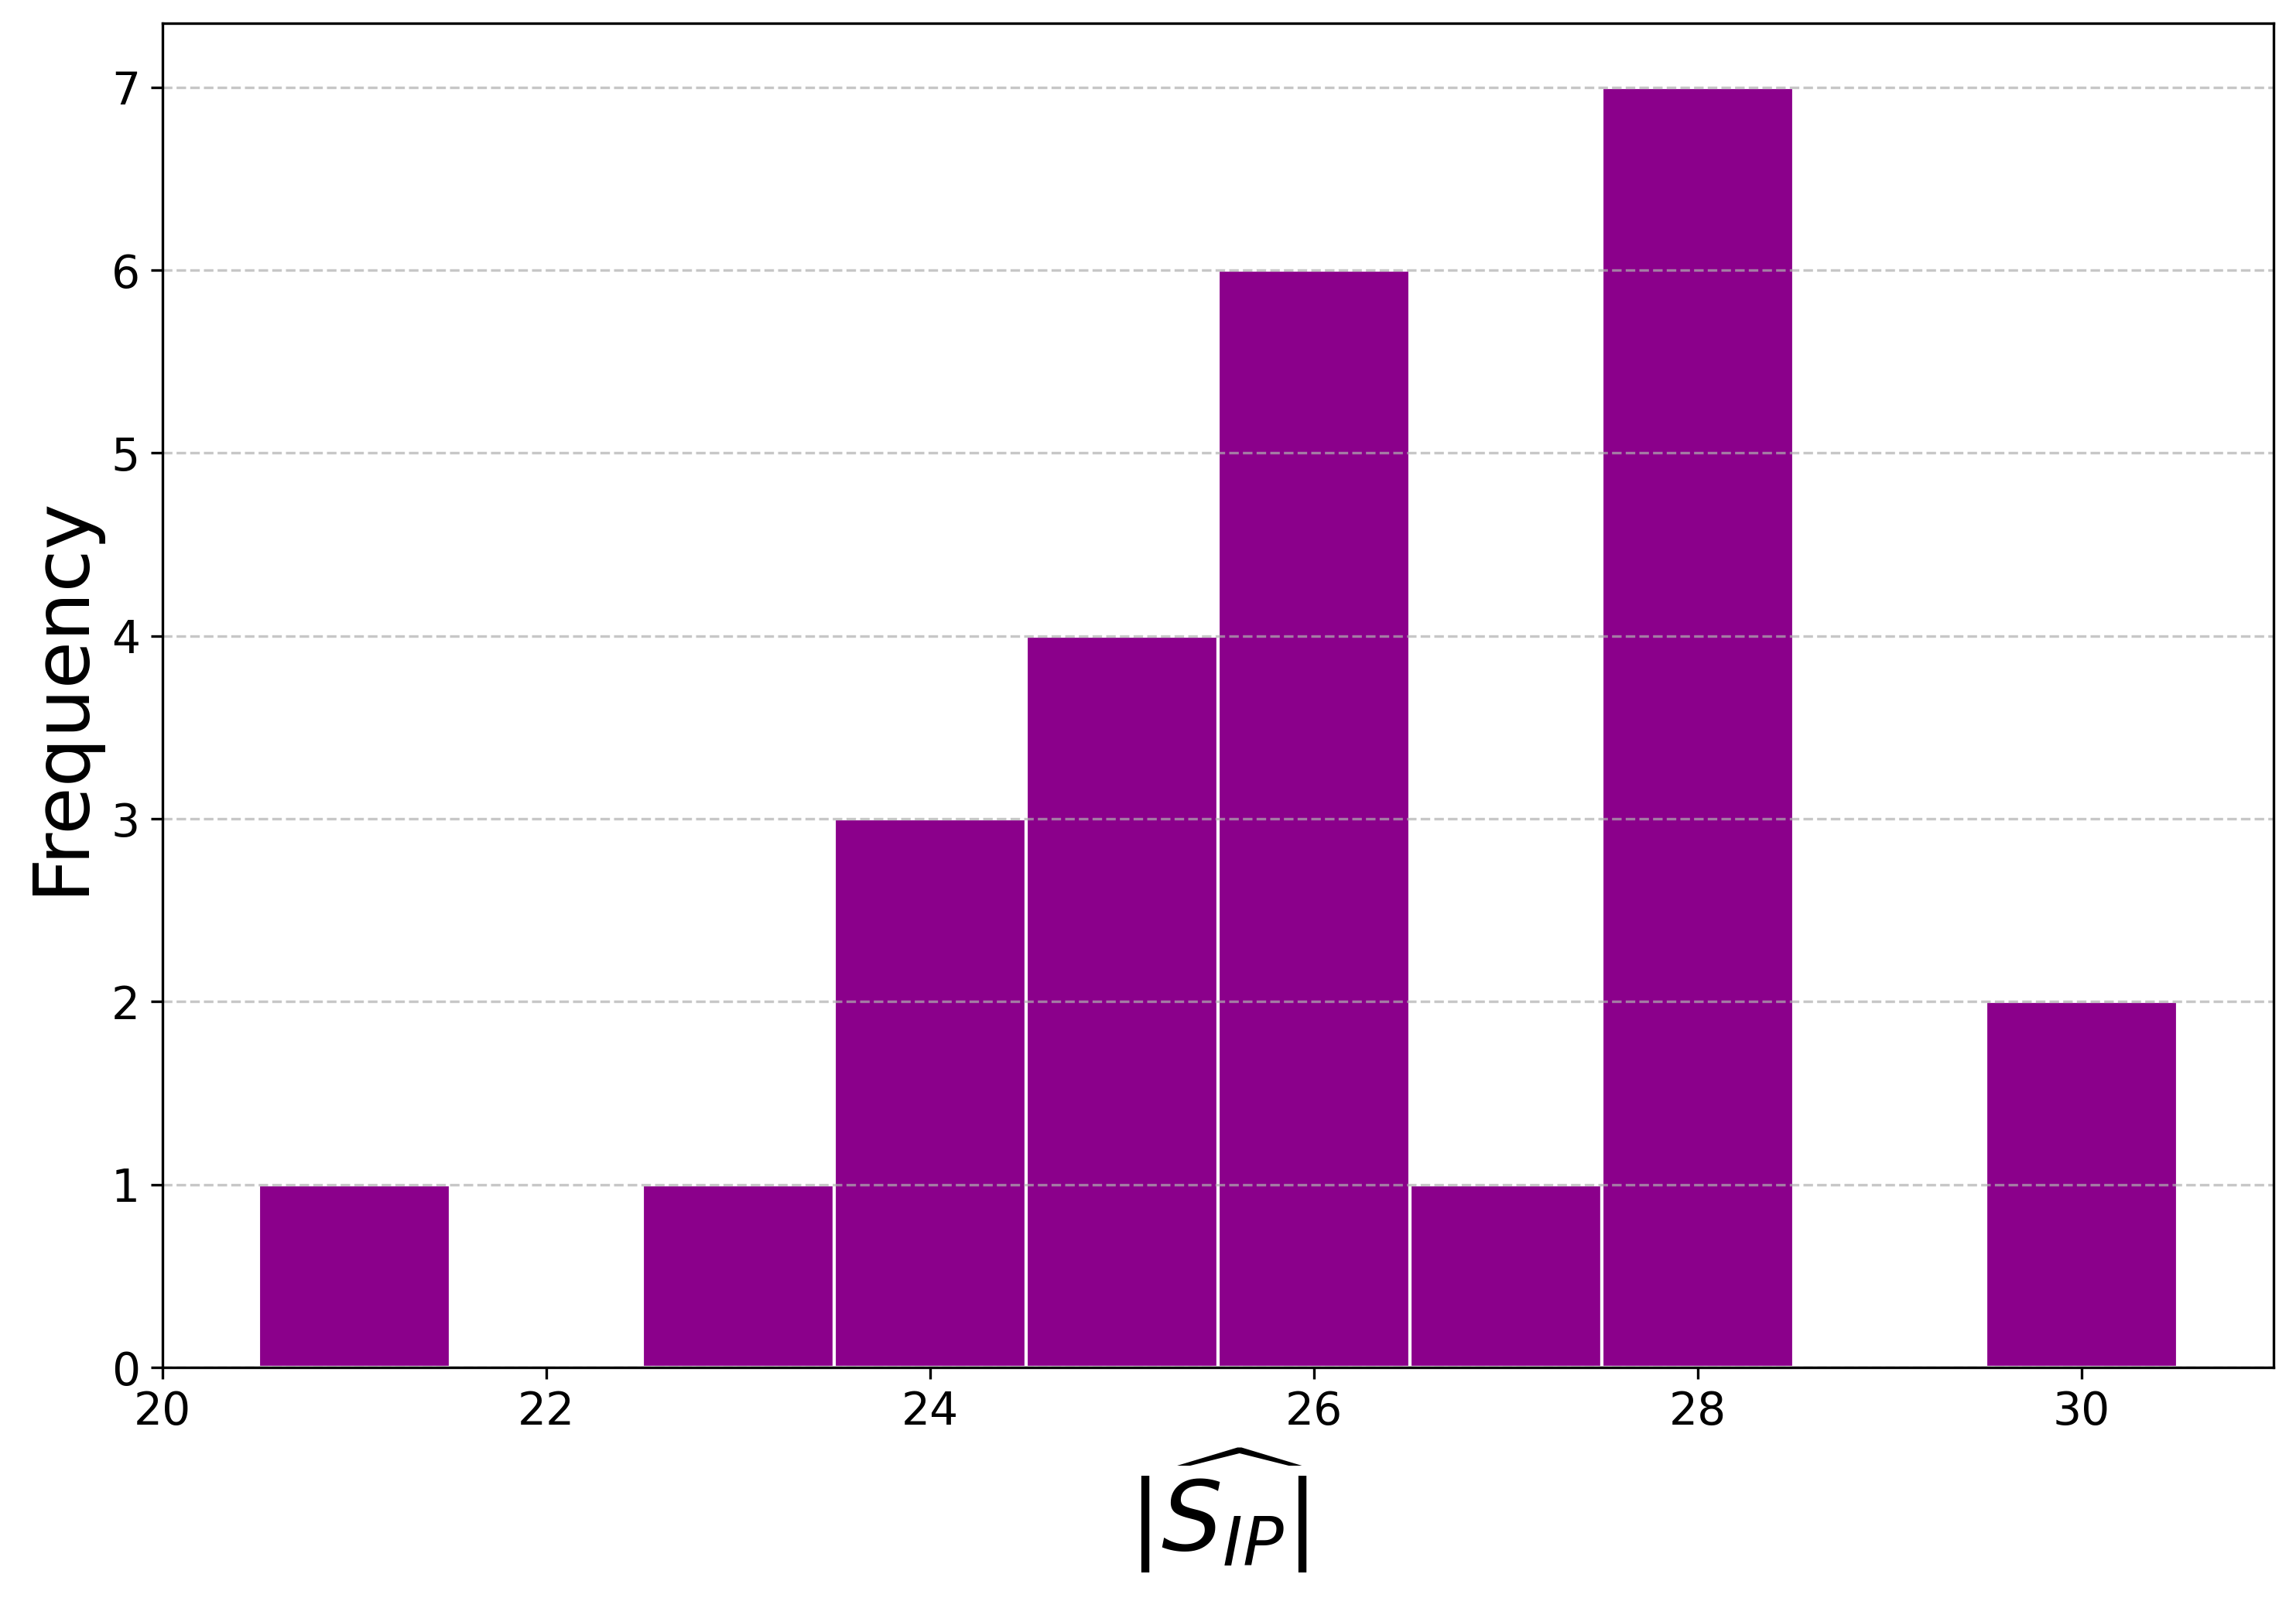
\includegraphics[width=\textwidth]{../figures/wine_cardinality_histogram.png}
\caption{Wine }
        \label{fig:wine_cardinalities}
    \end{subfigure}
    \hfill
    % Iris
    \begin{subfigure}[b]{0.32\textwidth}
        \centering
        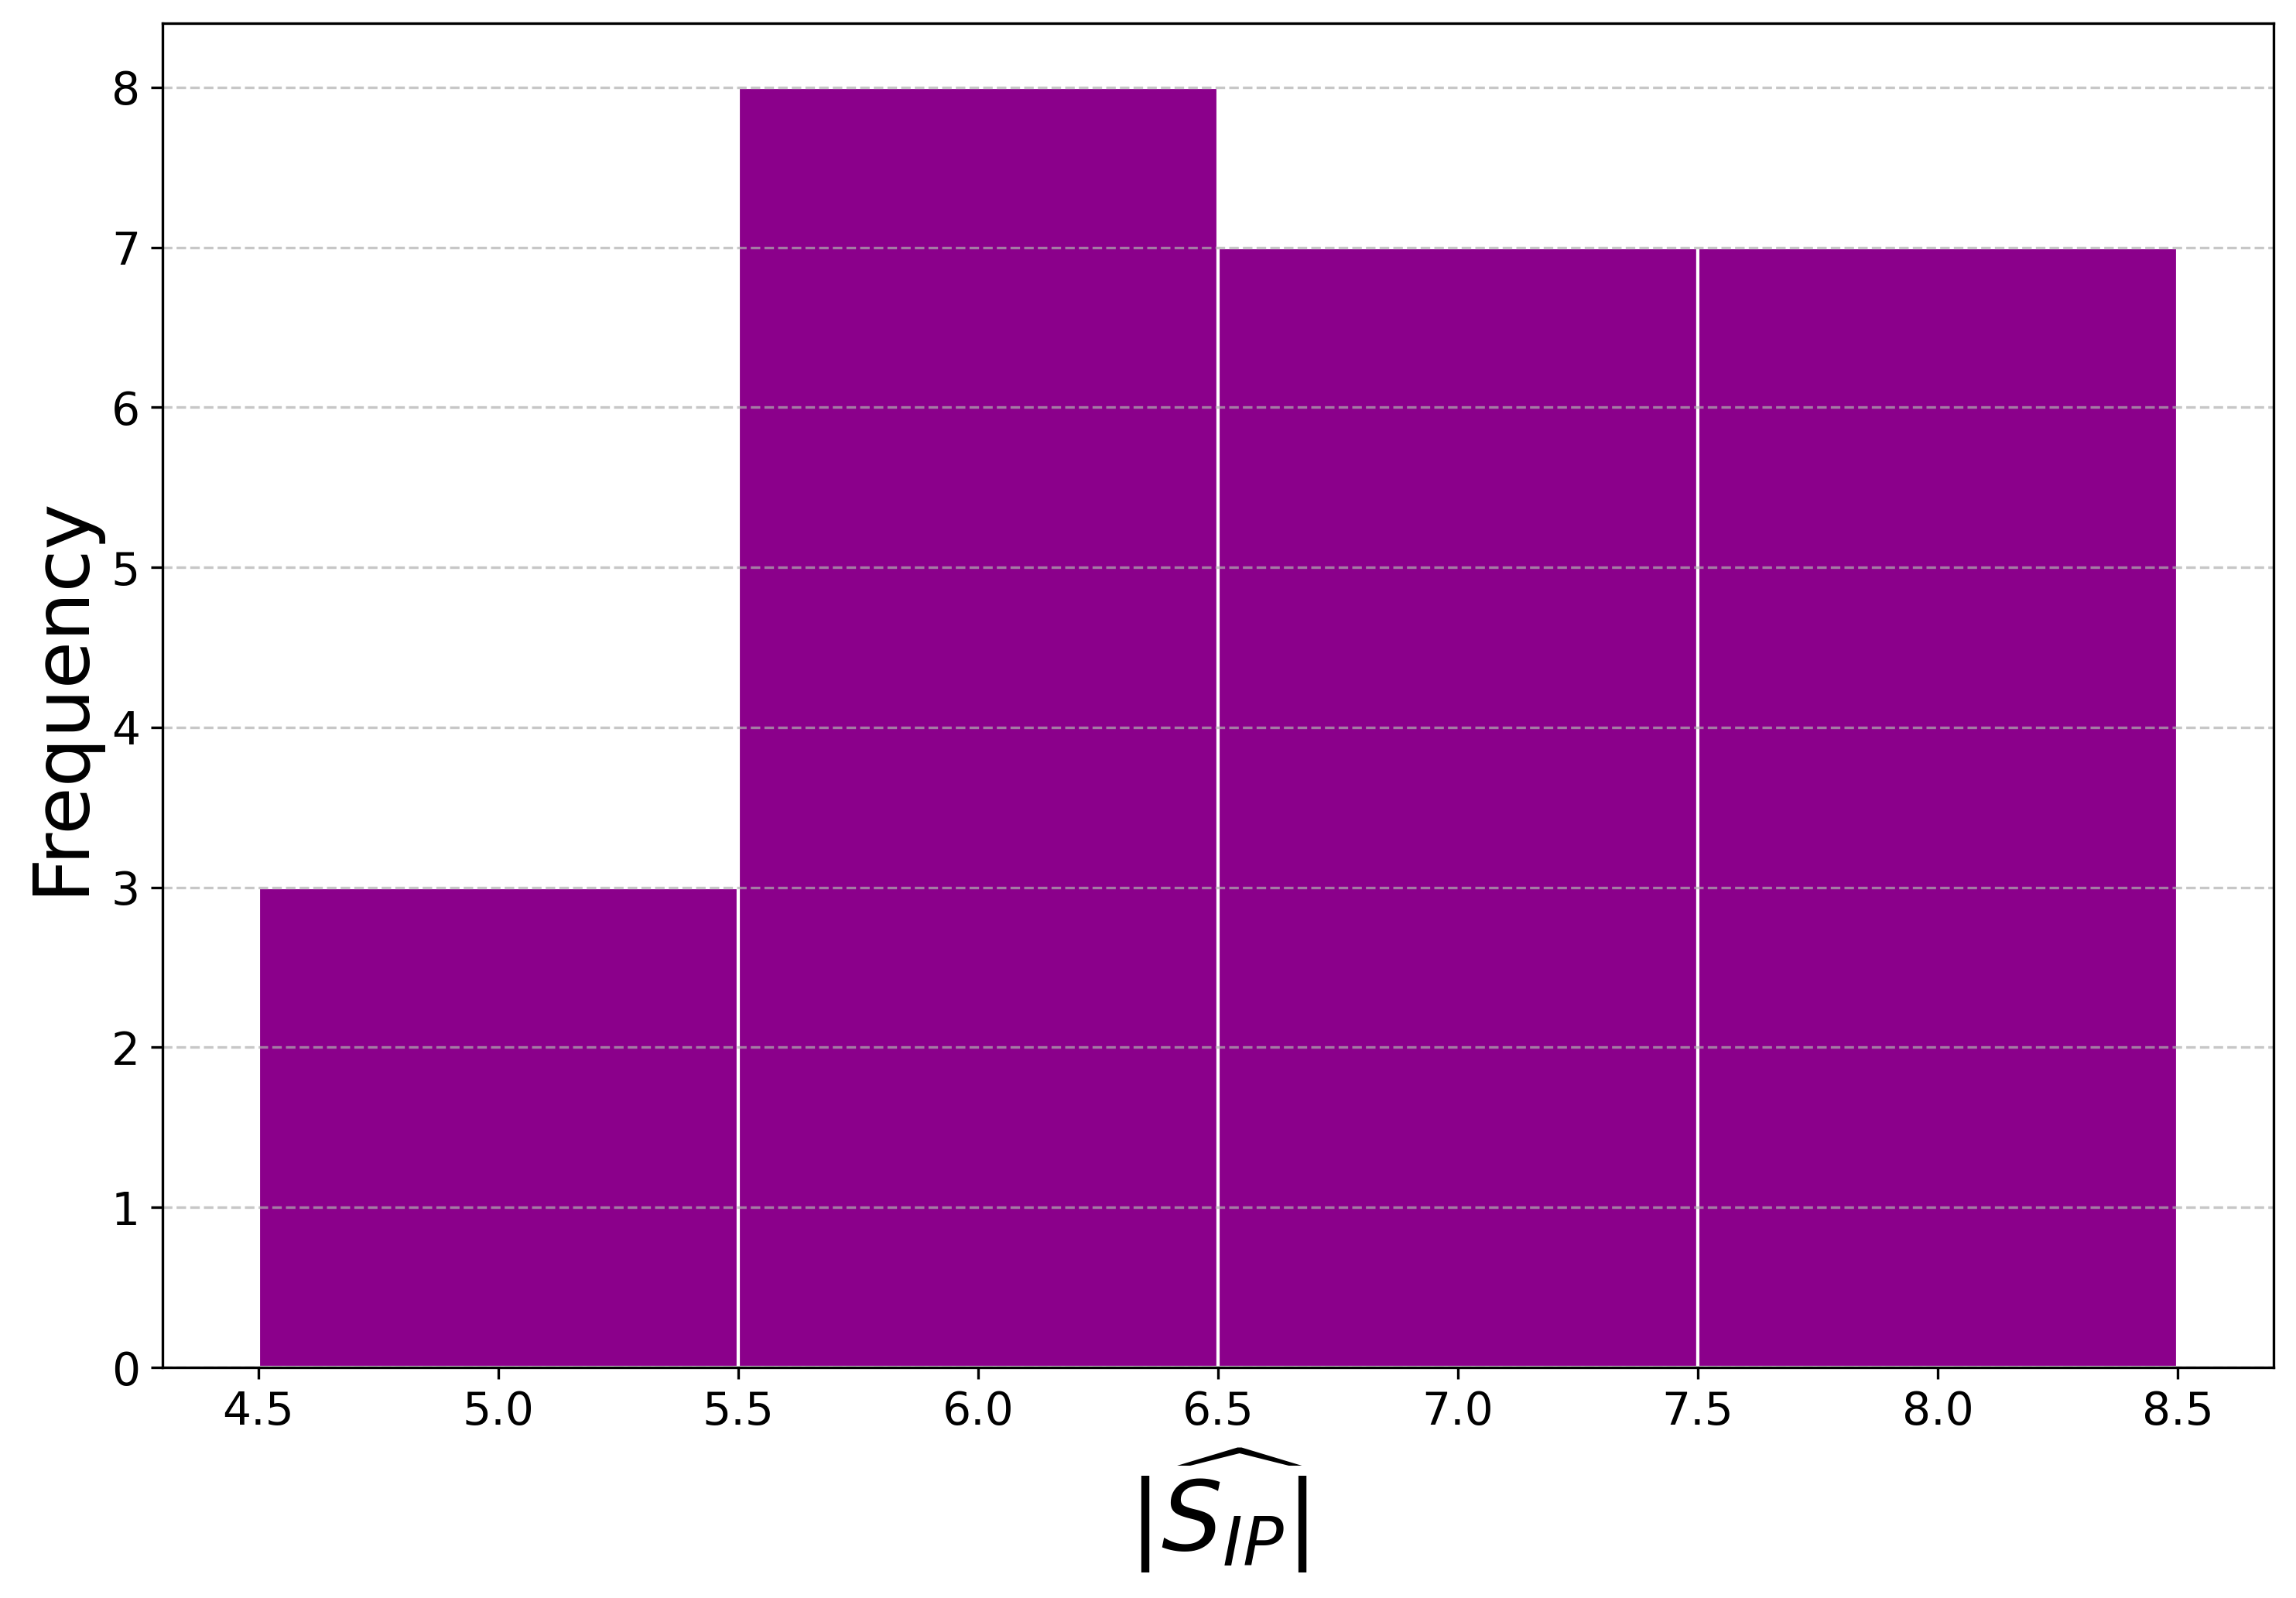
\includegraphics[width=\textwidth]{../figures/iris_cardinality_histogram.png}
\caption{Iris }
        \label{fig:iris_cardinalities}
    \end{subfigure}
    \hfill
    % Ethanol
    \begin{subfigure}[b]{0.32\textwidth}
        \centering
        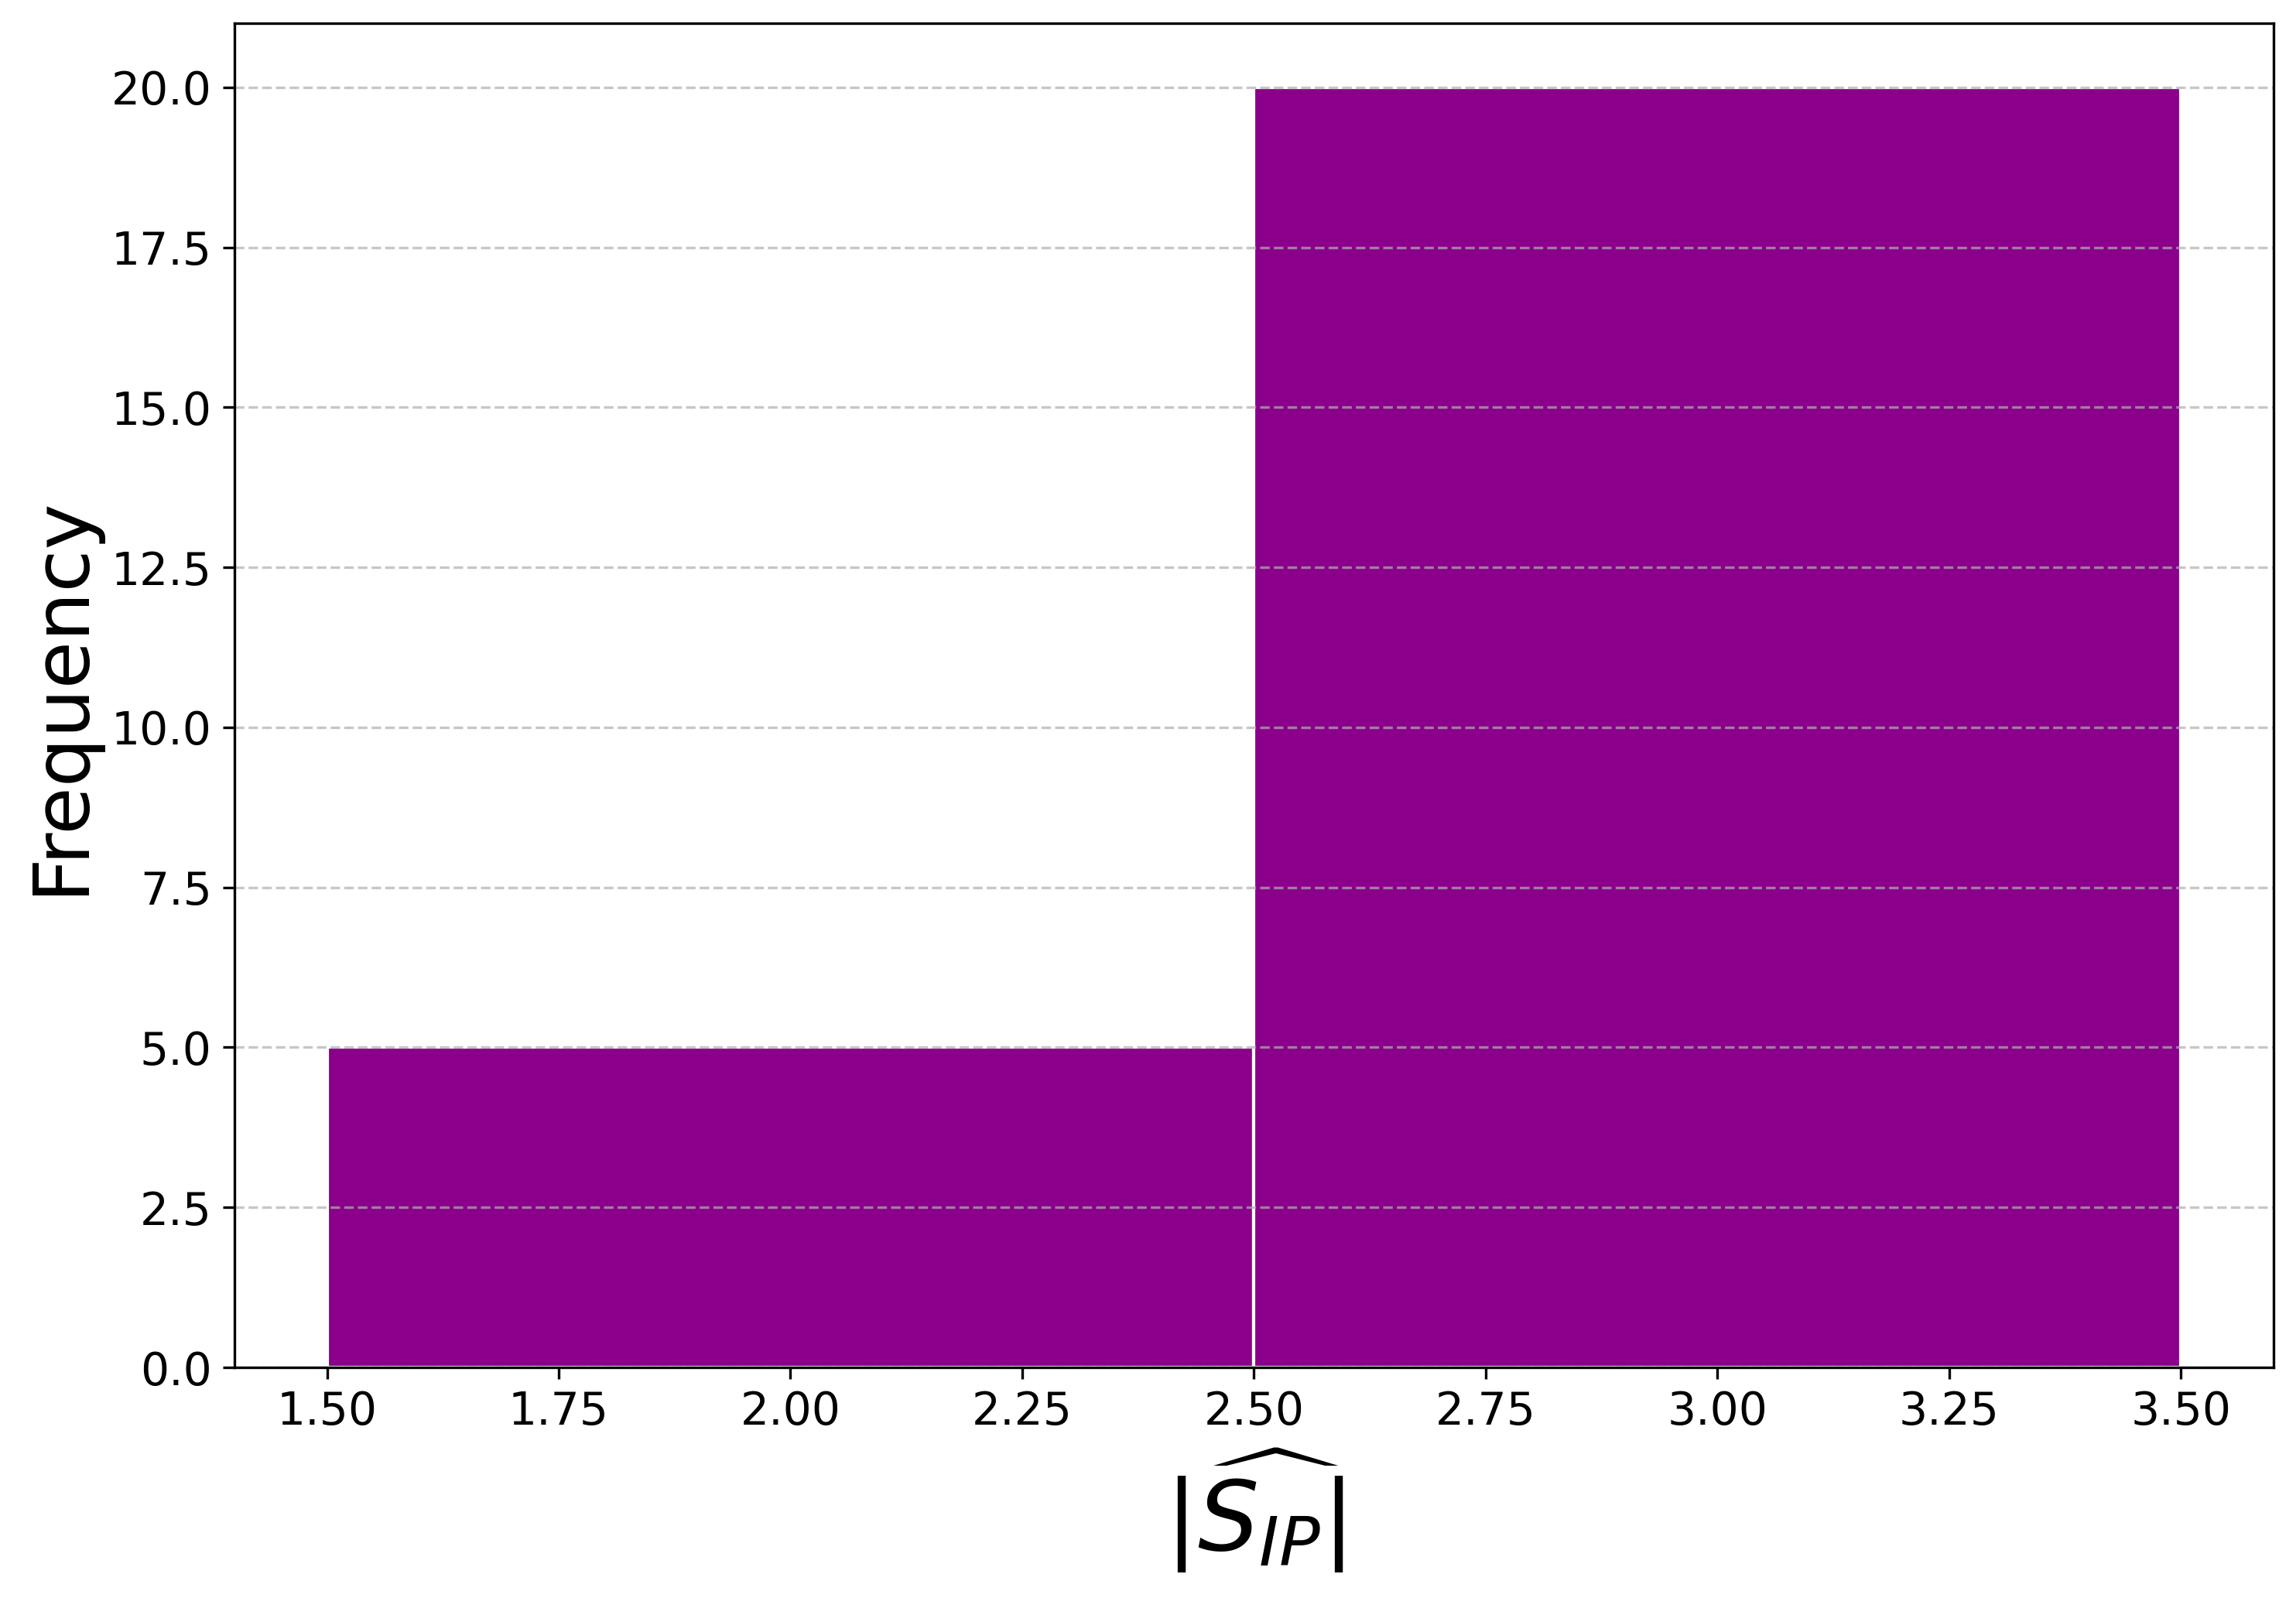
\includegraphics[width=\textwidth]{../figures/ethanol_cardinality_histogram.png}
\caption{Ethanol }
        \label{fig:ethanol_cardinalities}
    \end{subfigure}

\caption{Support cardinalities for each dataset after \isometrypursuit.}
    \label{fig:support_cardinalities}
\end{figure}

\newpage

\subsection{Timing}
\label{sec:timing}

While wall-time of algorithms is a non-theoretical quantity that depends on implementation details, it provides valuable context for practitioners.
We therefore report the following runtimes on a 2021 Macbook Pro.
The particularly high variance for brute force search in the second step of \tsip~ is likely due to the large cardinalities reported in Figure \ref{fig:support_cardinalities}.

\begin{table}[H]
\centering
\begin{tabular}{|c|c|c|c}
\toprule
Name & IP & 2nd stage & Greedy \\
\midrule
Iris & 1.24 ± 0.02 & 0.00 ± 0.00 & 0.02 ± 0.00 \\
Wine & 2.32 ± 0.17 & 0.13 ± 0.12 & 0.03 ± 0.00 \\
Ethanol & 8.38 ± 0.57 & 0.55 ± 1.08 & 0.07 ± 0.01 \\
\bottomrule
\end{tabular}
\caption{Algorithm runtimes in seconds across replicates.}
\end{table}



\begin{example}
    \begin{align}
        \label{prop:the_benzito}
        X_{S} = \begin{bmatrix}
        \frac{1}{2} & \frac{-1}{2} & \frac{1}{2} & \frac{-1}{2}  & \frac{1}{2} & \frac{-1}{2} \\
        \frac{\sqrt{3}}{2} & \frac{\sqrt{3}}{2} &0 & 0 \\
        0 & 0 &\frac{\sqrt{3}}{2} & \frac{\sqrt{3}}{2}  & 0& 0\\
        0& 0 0 & 0 &\frac{\sqrt{3}}{2} & \frac{\sqrt{3}}{2} \\
        \end{bmatrix}.
        \end{align}
\end{example}


\begin{proof}
Let
    
By Given the symmetry of the second and third columns around the y axis, the loss will not change regardless of whether we upweight one or downweight the other, these changes necessarily being in conjunction.
We therefore assume that their loadings with respect to the second column of the target matrix (the $D$ dimensional identity) are the same.
Clearly, they will both then have value of $\frac{1}{\sqrt{3}}$.
The question then becomes, what should the values of the first column in the loading matrix $\beta$ be?
    
We can answer this question with a simple differential equation.
Let $b$ denote the constraint violation $1 - X_{1.} \beta_{.1}$.
    
Then
    \begin{align}
        \frac{\partial b}{\partial \beta_{11}} = \frac{\partial b}{\partial\beta_{21}} \\
        &= \frac{1}{2}
    \end{align}
On the other hand, due to the value of $\frac{1}{\sqrt{3}}$ already assumed for the second loading of the second and third features,
    \begin{align}
        \frac{\partial l}{\partial \beta_{11}} &= \frac{\partial l}{\partial\beta_{21}} \\
        &= \frac{\partial }{\partial x}{\sqrt{\frac{1}{3} + x^2}} \\
        &= \frac{1}{2}(\frac{1}{3} + x^2)^{-\frac{1}{2}}(2x) \\
        &= \frac{x}{\sqrt{\frac{1}{3} + x^2}}.
    \end{align}
This means that the tradeoff
    \begin{align}
        \frac{\partial l}{\partial b} = \frac{1}{2x}\sqrt{\frac{1}{3} + x^2}.\
    \end{align}
In contrast, $\frac{\partial l}{\partial \beta_{11}} = 1$ and similarly for its constraint violation.
Solving for the equilibrium, we get
    \begin{align}
        \frac{1}{2x}\sqrt{\frac{1}{3} + x^2} = 1 \\
        \frac{1}{3} + x^2 = 4x^2 \\
        \frac{1}{3} = 3x^2 \\
        x = \frac{1}{\sqrt{3}}.
    \end{align}
This leads to a value for $l$ of
    \begin{align}
        \sqrt{\frac{1}{3} + \frac{1}{9}} + \sqrt{\frac{1}{3} + \frac{1}{9}} + \frac{2}{3} \\
        &=\sqrt{\frac{4}{9}} + \sqrt{\frac{4}{9}} + \frac{2}{3} \\
        &=\frac{2}{3} + \frac{2}{3} + \frac{2}{3} 
    \end{align}
    \end{proof}
    


\end{document}
